\documentclass[11pt,a4paper]{report}

% --------------------------
% --- Základní nastavení ---
% --------------------------
% Nastavení jazyka
\usepackage[czech]{babel}      % Czech language support
\usepackage[utf8]{inputenc}
\usepackage[T1]{fontenc}       % Proper Czech font encoding

\usepackage{csquotes}
\usepackage{amsmath,amssymb,latexsym,amsfonts}
% \usepackage{todonotes}
\usepackage{placeins} % Přidat do preambule
\usepackage{tabularx}
\usepackage{array}
\usepackage{pdfpages}  % Make sure this is in your preamble



% Přidání vlastních proměnných (jméno autora apod.)
\newcommand{\thesistype}{Diplomová práce}
\newcommand{\thesistopic}{Rozšíření modulární platformy pro elektromagnetické aktuátory}
\newcommand{\thesisdepartment}{KEP}
\newcommand{\thesisauthor}{Bc. Pavel Michalecký}
\newcommand{\thesissupervisor}{Ing. Martin Vítek}
\newcommand{\thesisconsultant}{Jméno konzultanta}





% ---------------------------
% --- Nastavení dokumentu ---
% ---------------------------
\usepackage{pdfpages}	% Obrázek přes celou stránku
\usepackage[top=2.3cm, left=2.5cm, right=2.5cm, bottom=2.3cm]{geometry}	% Definuje vzhled strany

\renewcommand{\baselinestretch}{1.5}
\setlength{\parskip}{1em} % Nastaveni mezer mezi odstavci
% \setlength{\parindent}{0pt} % Odstraní odsazení odstavců

\usepackage[nottoc,numbib]{tocbibind}	% Přidá odkaz na literaturu do obsahu
\usepackage{tocloft}	% Seznam obrázků, tabulek, obsah nemá číslo

% Definice barev
\definecolor{blue-light}{RGB}{91, 155, 213}
\definecolor{blue-FEL}{RGB}{7, 67, 145}
\definecolor{blue-dark}{RGB}{3, 31, 68}

\usepackage{indentfirst}	% Odsazeni prvního odstavce
\setcounter{secnumdepth}{3}	% Nastavení 3 podúrovní číslování nadpisu
\setcounter{tocdepth}{2}	% Nastaveni 2 podúrovní číslování nadpisu do obsahu
\renewcommand\labelitemi{--} % Nastaveni pomlčky

\usepackage{titlesec}		% Změna třídy chapter
\titlespacing*{\chapter}{0pt}{-25pt}{30pt}
\titleformat{\chapter}[hang]{\Huge\bfseries}{\thechapter\hspace{20pt}{}\hspace{20pt}}{0pt}{\Huge\bfseries}

% ---------------------------
% -- Obrázky, tabulky, ... --
% ---------------------------
\usepackage{graphicx}	% Vkládání obrázků, barvy
\usepackage{float}		% Možné umístění obrázků přesně kam chci + minipage
\usepackage[labelfont=bf]{caption} % Popisky obrázků s tučným úvodem
%\usepackage{url}
\usepackage{wrapfig}	% Obtékání textu kolem obrázku

\usepackage{tabularx}	% Lepší formátování tabulek
\usepackage{array}		% Lepší tabulky (zarovnání, šířka)
\usepackage{longtable}
\usepackage{booktabs}     % hezčí čáry


% Číslování obrázků, tabulek a rovnic 1,2,3 namísto 1.1, 1.2, 2.1
\renewcommand{\thefigure}{\arabic{figure}}
\renewcommand{\thetable}{\arabic{table}}
\renewcommand{\theequation}{\arabic{equation}}

% Čísla obrázků a tabulek rostou napříč více kapitolami (default je, že s každou sekcí se začíná od 1)
\usepackage{chngcntr}
\counterwithout{figure}{chapter}
\counterwithout{table}{chapter}
\counterwithout{equation}{chapter}

\usepackage{fancyref}	% Odkazy

\usepackage{listings}	% Kódy
\usepackage[framed,numbered,autolinebreaks,useliterate]{mcode}	% Formátování matlab kódu

% ---------------------------
% --- Jednotky a veličiny ---
% ---------------------------
\usepackage{siunitx}	% Formátování čísel s jednotkou (řeší nezalomitelné mezery, správné formátování jednotek apod.
\sisetup{product-units = single}	% Při dvou hodnotách vypíše jednotku jen na konci
\sisetup{mode=text,range-phrase = {\text{~až~}}, range-units=single}	% Při rozsahu vypíše mezi hodnotami "až"
\sisetup{output-decimal-marker = {,}}

\usepackage{textcomp}	% Aby gynsymb neukazoval error s \perthousand and \micro
\usepackage{gensymb}	% Symboly jako degree, micro atd.

% ---------------------------
% - Záhlaví, zápatí stránek -
% ---------------------------
\usepackage{fancyhdr}
\headheight 24pt	% nastavení výšky záhlaví

\renewcommand{\headrule}{\color{blue-light}{\rule{\textwidth}{0.5pt}}} % Redefinice barvy linky v záhlaví

\fancypagestyle{plain}{%
	\fancyhf{}

	\fancyhead[L]{{\scriptsize {\thesistopic}}}
	\fancyhead[R]{{\scriptsize {\thesisauthor, } \number\year}}

	\fancyfoot[C]{\thepage}
}

% -------------------------
% -- Nastavení řádkování --
% -------------------------
\usepackage{setspace}
%\singlespacing %jednoduche radkovani
\onehalfspacing %jedna a pul radkovani
%\doublespacing %dvojite radkovani

% --------------------------
% -- Nastavení literatury --
% --------------------------
\usepackage[
%	backend=bibtex,
	style=iso-numeric
]{biblatex}
\addbibresource{bib.bib}

% -------------------------------------
% - Nastavení výstupního PDF a odkazů -
% -------------------------------------
\usepackage[unicode]{hyperref} % měl by být načten jako jeden z posledních https://tex.stackexchange.com/questions/1863/which-packages-should-be-loaded-after-hyperref-instead-of-before
\hypersetup{
	colorlinks=true,
    linkcolor=blue-dark,
	citecolor=blue-dark,
	urlcolor=blue-FEL,
	pdfauthor={\thesisauthor},
	pdftitle={\thesistopic}
}
% --------------------------

%#######################################################################
%#   commands.tex  - Vlastní přikazy pro zpřehlednění výsledné práce   #
%#######################################################################

% -------------------------
% ------- Obrázky ---------
% -------------------------
% nový přikaz  \obr{velikost}{nazevobrazku s priponou}{popis obrazku}
% přiklad \obr{1}{obrazek}{Graf popisujici blabala....}


\DeclareSIUnit{\baud}{Bd}         % unit for modulation rate / line digit rate (13-16)

\newcommand{\obrH}[4]{\begin{figure}[H] % Pramatery H urcuje fixovani pozice obrazku na vlozenem miste 
		\centering
		\includegraphics[scale=#1]{#2}
		\caption{#3}
		\label{obr:#4}
	\end{figure}}

\newcommand{\obr}[4]{\begin{figure}
		\centering
		\includegraphics[scale=#1]{#2}
		\caption{#3}
		\label{obr:#4}
	\end{figure}}

% -------------------------
% --------- TODO ----------
% -------------------------
% Při odkomentování následujícího řádku můžete vkládat velmi jednoduché poznámky
\newcommand\todo[1]{\textcolor{red}{TODO: #1\newline}}

% Pro složitější tvorbu úkolů, odkomentujte následující 4 řádky. V kombinaci s tímto doporučujeme dočasně odkomentovat i styl/seznamy.tex a seznam TODO
%\usepackage[colorinlistoftodos,prependcaption,textsize=tiny]{todonotes}
%\usepackage{regexpatch}
%\makeatletter
%\xpatchcmd{\@todo}{\setkeys{todonotes}{#1}}{\setkeys{todonotes}{inline,#1}}{}{}

% Oba systémy úkolů se následně využívají takto:
%\todo{Chybí tu zmínit měření magnetického pole!}

% -------------------------
% -------- Nadpis ---------
% -------------------------
\newcommand{\nadpis}[1]{
	\noindent{\large{\textbf{#1}}}\\
}

% ----------------------------
%  Nastavení jednotek u rovnic 
% ----------------------------
\makeatletter
\providecommand\add@text{}
\newcommand\tagaddtext[1]{%
	\gdef\add@text{#1\gdef\add@text{}}}% 
\renewcommand\tagform@[1]{%
	\maketag@@@{\llap{\add@text\quad}(\ignorespaces#1\unskip\@@italiccorr)}%
}
\makeatother

\newcommand{\rov}[2]{
	\begin{equation}
		#1 \tagaddtext{($#2$)}
	\end{equation}
}   % Vlozeni vytorenych prikazu, ktere obsahuje soubor commands

% LaTeX Math Definitions

% Complex numbers
\newcommand{\cplx}[1]{{\underline{#1}}} % Complex number
\newcommand{\mi}{\mathrm{i}} % Complex unit
\newcommand{\mj}{\mathrm{j}} % Complex unit
\renewcommand{\Re}{\mathrm{Re}} % Real part
\renewcommand{\Im}{\mathrm{Im}} % Imaginary part

\newcommand{\phas}[1]{{\underline{#1}}} % Phasor
\newcommand{\vecphas}[1]{\mbox{\underline{\boldmath$#1$}}} % Phasor of vector
\newcommand{\faz}[1]{{\underline{#1}}} % Phasor
\newcommand{\vecfaz}[1]{\mbox{\underline{\boldmath$#1$}}} % Phasor of vector

% Vectors and matrices
\renewcommand{\vec}[1]{\mbox{\boldmath$#1$}} % Vector
\newcommand{\mat}[1]{\mathrm{\mathbf{{#1}}}} % Matrix, tenzor

% Diferential operators
\newcommand{\dif}{\,\mathrm{d}} % Differential
\newcommand{\grad}{\mathrm{grad}\ } % Gradient
\newcommand{\curl}{\mathrm{curl}\ } % Rotation
\renewcommand{\div}{\mathrm{div}\ } % Divergence

\newcommand{\laplace}{\triangle} % Laplace

% Others
\newcommand{\const}{\mathrm{const.}} % Constant
\newcommand{\konst}{\mathrm{konst.}} % Constant


\newcommand{\me}{\mathrm{e}} % Euler number

% Czech special definitions
\newcommand{\rot}{\mathrm{rot}\ } % Rotation
\newcommand{\tg}{\mathrm{tg}\ } % Tangens
\newcommand{\arctg}{\mathrm{arctg}\ }  % Vložení definic matematiky

%%%% NAVÍC %%%
% Reference příloh
\newcommand{\pref}[1]{příloha na straně \pageref{#1}, obr. \nameref{#1}}
\newcommand{\rref}[1]{rov. \eqref{#1}}
\newcommand{\oref}[1]{obr. \eqref{#1}}

\newcommand{\Pref}[1]{Příloha na straně \pageref{#1}, obr. \nameref{#1}}
\newcommand{\Rref}[1]{Rov. \eqref{#1}}
\newcommand{\Oref}[1]{Obr. \eqref{#1}}


% Listing
\lstset{literate=
    {á}{{\'a}}1 {č}{{\v{c}}}1 {ď}{{\v{d}}}1 {é}{{\'e}}1 {ě}{{\v{e}}}1 {í}{{\'i}}1 {ň}{{\v{n}}}1 
    {ó}{{\'o}}1 {ř}{{\v{r}}}1 {š}{{\v{s}}}1 {ť}{{\v{t}}}1 {ú}{{\'u}}1 {ů}{{\r{u}}}1 {ý}{{\'y}}1 {ž}{{\v{z}}}1
    {Á}{{\'A}}1 {Č}{{\v{C}}}1 {Ď}{{\v{D}}}1 {É}{{\'E}}1 {Ě}{{\v{E}}}1 {Í}{{\'I}}1 {Ň}{{\v{N}}}1 
    {Ó}{{\'O}}1 {Ř}{{\v{R}}}1 {Š}{{\v{S}}}1 {Ť}{{\v{T}}}1 {Ú}{{\'U}}1 {Ů}{{\r{U}}}1 {Ý}{{\'Y}}1 {Ž}{{\v{Z}}}1
}


\begin{document}

\begin{titlepage}
\begin{center}

	\textsc{\huge Západočeská univerzita v Plzni}

	%\textcolor[RGB]{91, 155, 213}{\rule{\textwidth}{1.5pt}}
	\textcolor{blue-light}{\rule{\textwidth}{1.5pt}}
    
    \Large{Fakulta elektrotechnická} \\
    \large{\thesisdepartment}

	\vspace{7cm}

	\Huge{\textsc{\textbf{\thesistype}}} \\
	\vspace{0.5cm}
	\Large{\thesistopic} \\
	
	\vfill

	\large
	\begin{tabular}{ m{4cm} m{6cm} } 
		Autor práce: & \textbf{\thesisauthor} \\
		Vedoucí práce: & \textbf{\thesissupervisor} \\
		% Konzultant práce: & \textbf{\thesisconsultant} \\
	\end{tabular}

	\textcolor[RGB]{91, 155, 213}{\rule{\textwidth}{1.5pt}}
	\Large\number\year

\end{center}

\cleardoublepage
\end{titlepage}



% V případě závěrečného projektu:
\clearpage

\pagenumbering{roman}

\chapter*{Zadání}

\begin{enumerate}
	\item Prostudujte ...
	\item Navrhněte ...
	\item Změřte ...
	\item Zhodnoťte ...
\end{enumerate}
% V případě DP:
\includepdf[pages={1}]{styl/zadani.pdf}

\pagestyle{plain}	% Odsud se budou aplikovat pravidla typu záhlaví, apod.

\clearpage

\pagenumbering{roman}

%ABSTRAKT

\chapter*{Abstrakt}

Tato diplomová práce se zabývá návrhem a realizací rozšířené verze \emph{modulární platformy MoSeZ} pro řízení elektromagnetických aktuátorů.
Hlavním cílem bylo rozšíření funkcí a zvýšení spolehlivosti původní verze MoSeZ Rev. A.

Vylepšení zahrnují novou revizi jednokanálového proudového zdroje s výstupním proudem až \SI{8}{\ampere},
podporu střídavého výstupu pomocí přímé digitální syntézy \emph{DDS} a implementaci softwarové \textit{PID} regulace ve firmwaru.

Modulární architektura byla zachována – vícekanálové systémy lze sestavit pomocí sběrnice \textit{CAN} a vlastního komunikačního protokolu.
Praktická část zahrnuje návrh \textit{DPS}, vývoj firmwaru v jazyce \textit{C++} a vývoj aplikace \textit{Staff 2.0} pro konfiguraci proudového výstupu zařízení.

Laboratorní měření prokázala přesnost řízení v režimech DC i AC.
Zařízení bylo úspěšně nasazeno k řízení čtyř voicecoilů ve vibračním podavači firmy \emph{DESSEQ}
a závěrem jsou nastíněny možné směry dalšího vývoje.

\vfill\section*{Klíčová slova}


proudový zdroj, elektromagnetické aktuátory, H-můstek, modulární platforma, PID regulace, přímá digitální syntéza, embedded systémy, CAN sběrnice


\vspace{1cm}

\newpage
\chapter*{Abstract}

This thesis deals with the design and implementation of an extended version of the \emph{modular MoSeZ} platform for controlling electromagnetic actuators.
The main objective was to extend the functionality and improve the reliability of the original MoSeZ Rev. A version.

Enhancements include a new revision of the single-channel current source with an output current up to \SI{8}{\ampere}, 
support for alternating output using direct digital synthesis \textit{DDS}, 
and the implementation of software-based \textit{PID} control in \textit{firmware}.

The modular architecture has been retained — multi-channel systems can be assembled using the \textit{CAN} bus and a custom communication protocol. 
The practical part includes the design of the \textit{PCB}, \textit{firmware} development in \textit{C++}, and the \textit{Staff 2.0} application for configuring the current output.

Laboratory measurements confirmed control precision in both DC and AC modes. 
The system was successfully deployed to control four voice coils in a \emph{DESSEQ} vibratory feeder, 
and possible directions for further development are outlined.


\vfill\section*{Keywords}
\noindent
current source, electromagnetic actuators, H-bridge, modular platform, PID control, direct digital synthesis, embedded systems, CAN bus
\vspace{1cm}

%PODEKOVANI

\newpage
\clearpage

\vspace*{3cm}
\section*{Poděkování}\vspace{1.5em}
\noindent
Rád bych poděkoval vedoucímu diplomové práce, \emph{Ing. Martinu Vítkovi}, za cenné odborné rady, vstřícný přístup a metodické vedení, 
které významně přispěly k úspěšnému dokončení této práce. Dále děkuji společnosti \emph{DESSEQ} za poskytnutí \emph{voicecoilů} a 
experimentálních vibračních stolic a za možnost ověřit návrh v praxi.  Poděkování patří také \emph{Ing. Zdeňku Kubíkovi, Ph.D.}, 
který umožnil měření vyzařování v EMC komoře. 
V neposlední řadě děkuji za sílu a vnitřní klid, které mi byly v průběhu práce dopřány z míst, jež přesahují každodennost.


\newpage
\clearpage

\vspace*{3cm}
\section*{Prohlášení}\vspace{1.5em}
\noindent
Během přípravy této práce autor použil \textit{ChatGPT} a \textit{Gemini AI}
k zlepšení čitelnosti a jazykové kvality rukopisu. 
Po použití tohoto nástroje/služby autor pečlivě zkontroloval a
upravil obsah podle potřeby a přebírá plnou odpovědnost za výsledný obsah práce.



% Tato diplomová práce se zaměřuje na návrh a realizaci rozšířené verze modulární platformy \emph{MoSeZ} určené pro řízení elektromagnetických aktuátorů. 
% Cílem práce bylo zvýšit modularitu, spolehlivost a funkční rozšiřitelnost původní verze zařízení \emph{MoSeZ Rev. A}, 
% a přizpůsobit ji pro širší spektrum technických aplikací.

% Navržená vylepšení zahrnují novou hardwarovou revizi jednokanálového proudového zdroje s výstupním proudem až \SI{8}{\ampere}, 
% doplněnou o podporu střídavých proudových výstupů pomocí přímé digitální syntézy (\emph{DDS}) a 
% řešení regulace pomocí softwarového \emph{PID} regulátoru.

% Významným aspektem návrhu je zachování modulární architektury platformy, 
% která umožňuje sestavení vícekanálového systému z jednotlivých jednokanálových modulů propojených pomocí průmyslové sběrnice \emph{CAN}. 
% Vlastní komunikační protokol založený na sběrnici \emph{CAN} zajišťuje kompatibilitu a integraci do rozsáhlejších systémů.

% Teoretická část práce se zabývá rešerší komunikačních protokolů využívajících sběrnici \emph{CAN}.
% Praktická část zahrnuje návrh desky plošných spojů, vývoj firmwaru v jazyce \emph{C++} a 
% tvorbu desktopové aplikace \emph{Staff 2.0} pro konfiguraci a diagnostiku proudového výstupu zařízení.

% Navržené řešení bylo ověřeno sérií laboratorních měření zaměřených na výstupní proud, 
% účinnost, harmonické zkreslení a přesnost regulace. 
% Výsledky prokázaly, že zařízení splňuje požadavky na přesné řízení elektromagnetických aktuátorů v režimech \emph{DC} i \emph{AC}.
% Zařízení bylo rovněž úspěšně nasazeno pro řízení čtyř voicecoilů v experimentálním vibračním podavači firmy \emph{DESSEQ}. 
% Závěrem je navrženo možné směřování dalšího vývoje platformy.

% \input{prohlaseni/prohlaseni.tex}

% Obsah, seznam obrázků, apod.
% -------------------------
% --------- Obsah ---------
% -------------------------
\cleardoublepage
\tableofcontents

% ------------------------
% ---- Seznam zkratek ----
% ------------------------
\newpage
\chapter*{Seznam použitých symbolů a zkratek}

% Přidat odkaz do obsahu
\addcontentsline{toc}{chapter}{Seznam použitých symbolů a zkratek}

\noindent

\begin{longtable}{@{}l p{10cm} c@{}}
	\toprule
	\textbf{Značka}    & \textbf{Popis}                                      & \textbf{Jednotka}                    \\
	\midrule
	\endfirsthead

	\toprule
	\textbf{Značka}    & \textbf{Popis}                                      & \textbf{Jednotka}                    \\
	\midrule
	\endhead

	\bottomrule
	\endfoot

	$\alpha$           & Koeficient EMA filtru                               & --                                   \\
	ac\_lut            & Tabulka průběhů pro DDS                             & --                                   \\
	$\beta$            & Koeficient derivačního filtru                       & --                                   \\
	$\Delta_{URIPPLE}$ & Zvlnění napětí                                      & \SI{}{V}                             \\
	$\Delta U_{BSTQ}$  & Přípustný pokles bootstrap napětí                   & \SI{}{V}                             \\
	$\Delta \varphi$   & Fázový přírůstek DDS                                & --                                   \\
	$\eta$             & Účinnost                                            & \SI{}{\percent}                      \\
	AC                 & Střídavý proud                                      & \SI{}{\ampere}                       \\
	ADC                & Analogově-digitální převodník                       & --                                   \\
	Airflow            & Průtok vzduchu (pro chlazení)                       & --                                   \\
	ATSAME51J20A       & Mikrokontrolér                                      & --                                   \\
	BYG10D             & Ochranná dioda                                      & --                                   \\
	CAD                & Počítačem podporované návrhářství                   & --                                   \\
	CAN                & Controller Area Network                             & --                                   \\
	CANopen            & Komunikační protokol založený na CAN                & --                                   \\
	CCx                & Capture/Compare registr                             & --                                   \\
	CIP                & Common Industrial Protocol                          & --                                   \\
	CiA                & CAN in Automation (organizace)                      & --                                   \\
	C++                & Programovací jazyk používaný pro firmware           & --                                   \\
	$C_{IN}$           & Kapacita vstupního kondenzátoru                     & \SI{}{F}                             \\
	$C_{bootstrap}$    & Bootstrap kondenzátor                               & \SI{}{F}                             \\
	$C_{OUT}$          & Výstupní filtrační kondenzátor                      & \SI{}{F}                             \\
	CompoNet           & Průmyslová síť                                      & --                                   \\
	ControlNet         & Průmyslová síť                                      & --                                   \\
	DC                 & Stejnosměrný proud                                  & \SI{}{\ampere}                       \\
	DDS                & Přímá digitální syntéza                             & --                                   \\
	DESSEQ             & Firma zabývající se automatizací a robotizací       & --                                   \\
	DeviceNet          & Průmyslový komunikační protokol                     & --                                   \\
	$D_{max}$          & Maximální střída PWM signálu                        & --                                   \\
	DPS                & Deska plošného spoje                                & --                                   \\
	DPLL               & Digitální fázový závěs                              & --                                   \\
	$DC_{OFFSET}$      & Stejnosměrný offset                                 & \SI{}{\ampere}                       \\
	ECC                & Error Correction Code                               & --                                   \\
	EMC                & Elektromagnetická kompatibilita                     & --                                   \\
	EMCY               & Emergency message (CANopen)                         & --                                   \\
	EMI                & Elektromagnetické rušení                            & --                                   \\
	EMA                & Exponenciální klouzavý průměr                       & --                                   \\
	ESD                & Elektrostatický výboj                               & --                                   \\
	EtherCAT           & Průmyslový ethernetový protokol                     & --                                   \\
	EtherNet/IP        & Průmyslový ethernetový protokol                     & --                                   \\
	EVSYS              & Event System v mikrokontroléru ATSAME51             & --                                   \\
	$f_{CLK}$          & Taktovací frekvence                                 & \SI{}{\hertz}                        \\
	$f_{CM}$           & Zlomová frekvence Common-mode filtru                & \SI{}{\hertz}                        \\
	$f_{DM}$           & Zlomová frekvence Differential-mode filtru          & \SI{}{\hertz}                        \\
	$f_{OUT}$          & Výstupní frekvence                                  & \SI{}{\hertz}                        \\
	$f_{SW}$           & Spínací frekvence                                   & \SI{}{\hertz}                        \\
	FIFO               & First In First Out buffer                           & --                                   \\
	FW ARON            & firmware platformy MoSeZ                            & --                                   \\
	GCLK               & Generický hodinový generátor                        & --                                   \\
	GUI                & Graphical User Interface                            & --                                   \\
	HB                 & Heartbeat zpráva                                    & --                                   \\
	$h_{LAYER}$        & Výška vrstvy tisku                                  & \SI{}{\milli\meter}                  \\
	Honeycomb          & Voštinový vzor výplně 3D tisku                      & --                                   \\
	I/O                & Vstup/výstup                                        & --                                   \\
	ID                 & Identifikátor zařízení                              & --                                   \\
	IEEE 802.3         & Ethernet standard                                   & --                                   \\
	$I_1$              & Základní harmonická složka                          & \SI{}{\ampere} nebo \SI{}{\deci\bel} \\
	$I_{DDQ}$          & Klidový proud high-side budiče                      & \SI{}{\ampere}                       \\
	$I_{BSTQ}$         & Klidový proud bootstrap obvodu                      & \SI{}{\ampere}                       \\
	$I_{EF}$           & Efektivní hodnota proudu                            & \SI{}{\ampere}                       \\
	INA241B1           & Verze senzoru proudu INA241                         & --                                   \\
	Infill             & Procento výplně modelu                              & \SI{}{\percent}                      \\
	ISC080N10          & MOSFET tranzistor                                   & --                                   \\
	ISO/OSI            & Referenční model pro síťovou komunikaci             & --                                   \\
	$I_{SET}$          & Nastavený proud                                     & \SI{}{\ampere}                       \\
	$I_{LOAD}$         & Proud zátěže                                        & \SI{}{\ampere}                       \\
	$I_{OUT}$          & Výstupní proud                                      & \SI{}{\ampere}                       \\
	$I_{RIPPLE}$       & Zvlnění proudu                                      & \SI{}{\ampere}                       \\
	$I_{RMS}$          & Efektivní hodnota proudu                            & \SI{}{\ampere}                       \\
	IRT                & Isochronous Real Time (PROFINET)                    & --                                   \\
	K                  & Koeficient zvlnění proudu                           & --                                   \\
	L                  & Indukčnost výstupního filtru                        & \SI{}{\henry}                        \\
	LMR38010           & Synchronní snižující měnič                          & --                                   \\
	LM78M33            & Lineární stabilizátor napětí                        & --                                   \\
	$L_{LOAD}$         & Indukčnost zátěže                                   & \SI{}{\henry}                        \\
	LUT                & Look-Up Table                                       & --                                   \\
	MAC ID             & Media Access Control Identifier                     & --                                   \\
	MCU                & Mikrokontrolér                                      & --                                   \\
	MCP1501T           & Přesná napěťová reference                           & --                                   \\
	MoSeZ              & Platforma modulárních spínaných zdrojů              & --                                   \\
	MP1917             & Budič MOSFET tranzistorů                            & --                                   \\
	MP2344             & Snižující měnič (původní verze)                     & --                                   \\
	NMT                & Network Management (CANopen)                        & --                                   \\
	NRF                & Non-Recoverable Fault                               & --                                   \\
	NVMCTRL            & Řadič nonvolatilní paměti                           & --                                   \\
	OD                 & Object Dictionary (CANopen)                         & --                                   \\
	Onshape            & Online CAD software                                 & --                                   \\
	OpenPnP            & Open-source osazovací automat                       & --                                   \\
	OTMX               & Output Matrix                                       & --                                   \\
	$P_{D\_MAX}$       & Maximální ztrátový výkon                            & \SI{}{\watt}                         \\
	PETG               & Polyethylentereftalát glykol                        & --                                   \\
	PHASE\_ACCUM       & Fázový akumulátor DDS                               & --                                   \\
	PHASE\_INC         & Fázový přírůstek DDS                                & --                                   \\
	PID                & Proporcionálně-integračně-derivační regulátor       & --                                   \\
	$P_G$              & Ztráty hradlem MOSFET tranzistoru                   & \SI{}{\watt}                         \\
	$P_{DO}$           & Process Data Object (CANopen)                       & --                                   \\
	$P_{IN}$           & Vstupní výkon                                       & \SI{}{\watt}                         \\
	$P_J$              & Vodivostní ztráty MOSFET tranzistoru                & \SI{}{\watt}                         \\
	$P_{LOSS}$         & Celkové ztráty na MOSFET tranzistoru                & \SI{}{\watt}                         \\
	$P_{OUT}$          & Výstupní výkon                                      & \SI{}{\watt}                         \\
	$P_{SW}$           & Spínací ztráty MOSFET tranzistoru                   & \SI{}{\watt}                         \\
	PROFIBUS           & Průmyslová sběrnice                                 & --                                   \\
	PROFINET           & Průmyslový komunikační protokol                     & --                                   \\
	Prusa Mk4          & Model 3D tiskárny                                   & --                                   \\
	PTC                & Positive Temperature Coefficient                    & --                                   \\
	PTH                & Technologie průchozí montáže                        & --                                   \\
	PWM                & Pulsně šířková modulace                             & --                                   \\
	$Q_G$              & Celkový náboj hradla                                & \SI{}{\coulomb}                      \\
	$Q_{total}$        & Celkový náboj pro bootstrap                         & \SI{}{\coulomb}                      \\
	RAM                & Random Access Memory                                & --                                   \\
	Reflow             & Pájecí proces SMT součástek                         & --                                   \\
	$R_{CM}$           & Odpor common-mode filtru                            & \SI{}{\ohm}                          \\
	$R_{DM}$           & Odpor differential-mode filtru                      & \SI{}{\ohm}                          \\
	$R_{DS\_ON}$       & Odpor kanálu MOSFET tranzistoru                     & \SI{}{\ohm}                          \\
	$R_{FBT}$          & Horní zpětnovazební odpor                           & \SI{}{\ohm}                          \\
	$R_{FBB}$          & Dolní zpětnovazební odpor                           & \SI{}{\ohm}                          \\
	$R_{LOAD}$         & Odpor zátěže                                        & \SI{}{\ohm}                          \\
	RMS                & Efektivní hodnota                                   & --                                   \\
	$R_{SENSE}$        & Snímací odpor pro měření proudu                     & \SI{}{\ohm}                          \\
	$R_{T}$            & Terminační odpor pro nastavení spínacího kmitočtu   & \SI{}{\ohm}                          \\
	RT                 & Real Time (PROFINET)                                & --                                   \\
	$R_{THJA}$         & Tepelný odpor tranzistor-okolí                      & \SI{}{\kelvin\per\watt}              \\
	SERCOM             & Sériová komunikační periferie                       & --                                   \\
	SDO                & Service Data Object (CANopen)                       & --                                   \\
	SIN                & Harmonický (sinusový) průběh                        & --                                   \\
	SMD                & Surface-mount device                                & --                                   \\
	SMT                & Technologie povrchové montáže                       & --                                   \\
	SP/SH/SW           & Sekvenční příkazy                                   & --                                   \\
	SQUARE             & Obdélníkový průběh                                  & --                                   \\
	Staff 2.0          & Řídicí aplikace pro MoSeZ                           & --                                   \\
	ST/SC/SF           & Příkazy pro řízení sekvencí                         & --                                   \\
	SYNC               & Synchronizační zpráva                               & --                                   \\
	$T_{BED}$          & Teplota podložky tisku                              & \SI{}{\celsius}                      \\
	$T_J$              & Teplota přechodu tranzistoru                        & \SI{}{\celsius}                      \\
	$T_{J\_MAX}$       & Maximální teplota přechodu                          & \SI{}{\celsius}                      \\
	$T_{PRINT}$        & Teplota tisku                                       & \SI{}{\celsius}                      \\
	TCAN334G           & CAN transceiver                                     & --                                   \\
	TCx                & Časovač/čítač                                       & --                                   \\
	TCCx               & Časovač pro PWM                                     & --                                   \\
	TCP/IP             & Transmission Control Protocol/Internet Protocol     & --                                   \\
	Temp               & Teplota                                             & \SI{}{\celsius}                      \\
	THD                & Celkové harmonické zkreslení                        & \SI{}{\percent}                      \\
	THT                & Through-hole technology                             & --                                   \\
	TRIANGLE           & Trojúhelníkový průběh                               & --                                   \\
	TVS                & Transient Voltage Suppressor dioda                  & --                                   \\
	$U_{ADC}$          & Naměřené napětí z ADC                               & \SI{}{\volt}                         \\
	$U_{BSC}$          & Napětí na bootstrap kondenzátoru                    & \SI{}{\volt}                         \\
	$U_{D}$            & Úbytek napětí na diodě                              & \SI{}{\volt}                         \\
	$U_{DH}$           & Úbytek napětí na bootstrap diodě                    & \SI{}{\volt}                         \\
	UDP                & User Datagram Protocol                              & --                                   \\
	$U_{GS}$           & Napětí hradlo-source tranzistoru                    & \SI{}{\volt}                         \\
	$U_{HT}$           & Hystereze podpěťové ochrany budiče                  & \SI{}{\volt}                         \\
	$U_{IN}$           & Vstupní napětí                                      & \SI{}{\volt}                         \\
	$U_{LS}$           & Napětí na low-side tranzistoru                      & \SI{}{\volt}                         \\
	$U_{MAX}$          & Maximální napětí v LUT                              & \SI{}{\volt}                         \\
	$U_{MIN}$          & Minimální napětí v LUT                              & \SI{}{\volt}                         \\
	$U_{OUT}$          & Výstupní napětí                                     & \SI{}{\volt}                         \\
	$U_{REF}$          & Referenční napětí                                   & \SI{}{\volt}                         \\
	$U_T$              & Prahové napětí MOSFET tranzistoru                   & \SI{}{\volt}                         \\
	$U_{UPFT}$         & Prahová hodnota podpěťové ochrany budiče            & \SI{}{\volt}                         \\
	$U_{UPRT}$         & Prahová hodnota podpěťové ochrany při náběhu napětí & \SI{}{\volt}                         \\
	UART               & Univerzální asynchronní přijímač/vysílač            & --                                   \\
	USB-CAN            & Převodník USB na CAN                                & --                                   \\
	USB-UART           & Převodník USB na UART                               & --                                   \\
	USERROW            & Uživatelská řádka v paměti                          & --                                   \\
	$V_{PRINT}$        & Rychlost tisku                                      & \SI{}{\milli\meter\per\second}       \\
	Voicecoil          & Lineární elektromagnetický aktuátor                 & --                                   \\
	WDT                & Watchdog Timer                                      & --                                   \\
	X7R                & Typ keramického dielektrika                         & --                                   \\
\end{longtable}

% ------------------------
% ---- Seznam TODO ----
% ------------------------
% Pokud byste si chtěli zobrazit všechny TODO na jednom místě
%\newpage
%\listoftodos


% ------------------------
% ---- Seznam obrázků ----
% ------------------------
\newpage
\listoffigures

% ------------------------
% ---- Seznam tabulek ----
% ------------------------
\newpage
\listoftables


% -------------------------
% ----- Seznam rovnic -----
% -------------------------
%\newpage
%\newcommand{\listequationsname}{List of Equations}
%\newlistof{myequations}{equ}{\listequationsname}
%\newcommand{\myequations}[1]{%
%\addcontentsline{equ}{myequations}{\protect\numberline{\theequation}#1}\par}
%\setlength{\cftmyequationsnumwidth}{2.5em}% Width of equation number in List of Equations






\newpage
\pagenumbering{arabic}	% Změna stylu číslování stran.

\chapter*{Úvod}
\addcontentsline{toc}{chapter}{Úvod} % Přidá úvod do obsahu

S rostoucími nároky na přesnost, spolehlivost a škálovatelnost řízení elektromagnetických aktuátorů se zvyšuje potřeba vysoce flexibilních a
snadno rozšiřitelných řídicích platforem.
Tyto požadavky se objevují napříč obory -- od průmyslové automatizace až po vývoj pokročilých mechatronických systémů.
Modulární platforma \textit{MoSeZ} představuje řešení pro řízení proudových výstupů,
které umožňuje efektivní správu aktuátorů s využitím průmyslové sběrnice \textit{CAN}.

Původní verze zařízení \textit{MoSeZ Rev. A} byla navržena pro napájení \SI{12}{\volt} a umožňovala pouze stejnosměrný výstup. 
Vzhledem k požadavku vyššího napájecího rozsahu, podpory střídavých signálů a 
možnosti zpětné vazby z řízeného systému však bylo nutné připravit rozšířenou variantu platformy.

Tato práce se proto zaměřuje na návrh hardwarového a softwarového rozšíření platformy \textit{MoSeZ} tak, 
aby podporovala napájecí napětí v rozsahu od \SI{12}{\volt} do \SI{48}{\volt},
umožňovala generovat střídavý proud prostřednictvím přímé digitální syntézy (\textit{DDS}) a
byla připravena pro zavedení zpětné vazby z řízených aktuátorů – například informace o stavu ventilu (otevřený/zavřený) nebo poloze jádra.
Klíčovým požadavkem také bylo zachování modulární architektury,
která umožňuje sestavení vícekanálového systému z jednotlivých jednokanálových modulů.

Součástí práce je návrh a vývoj nezbytných podpůrných komponent:
desky plošných spojů, firmwaru, vlastního komunikačního protokolu založeného na sběrnici \textit{CAN},
nasazení modulů do experimentálního zařízení a následného zkoušení a testování celého systému.

Cílem práce je vytvořit robustní,
modulární a konfigurovatelný řídicí systém pro elektromagnetické aktuátory,
který bude připraven pro snadnou integraci do rozsáhlejších experimentálních sestav.
\newpage

\chapter{Komunikační protokoly založené na sběrnici \textit{\textit{CAN} }}

Sběrnice \textit{CAN} (Controller Area Network) byla původně vyvinuta společností Bosch pro automobilový průmysl jako řešení rostoucí složitosti kabelových rozvodů.
Její robustní návrh a efektivita vedly k širokému nasazení i v dalších oblastech průmyslové automatizace.
Mezi klíčové vlastnosti této sběrnice patří:

\begin{itemize}
	\item \textbf{Robustní fyzická vrstva:}  Je navržen pro spolehlivý provoz v náročných průmyslových prostředích.
	\item \textbf{Nízká režie:} Protokol  má relativně nízkou režii, což znamená efektivní využití přenosového média.
	\item \textbf{Jednoduché rozhraní:} Implementace  nevyžaduje rozsáhlé hardwarové prostředky,
	      často postačuje i méně výkonný 8-bitový mikroprocesor s malou pamětí (řádově \SI{4}{\kilo\byte} programové paměti a \SI{256}{\byte} \textit{RAM}).
	\item \textbf{Bitová arbitráž:}  Využívá nedestruktivní bitovou arbitráž pro řízení přístupu k síti.
	      Pokud více uzlů započne vysílání současně, arbitrážní mechanismus zajistí,
	      že zpráva s vyšší prioritou (definovanou identifikátorem) získá přístup k sběrnici bez ztráty dat.
	      Vítězný uzel pokračuje ve vysílání, zatímco ostatní uzly, které prohrály arbitráž, se stáhnou a čekají na uvolnění sběrnice.
	      Uzel může započít vysílání jen pokud je sběrnice uvolněna.
	      Pokud začne uzel s vyšším \textit{ID} (nižší prioritou) úspěšně vysílat,
	      musí všechny ostatní uzly čekat na uvolnění sběrnice,
	      bez ohledu na jejich \textit{ID} (prioritu).
	\item \textbf{Datové a vzdálené rámce:}  Definuje formáty zpráv,
	      jako je datový rámec (pro přenos dat) a vzdálený rámec (pro vyžádání dat).
	\item \textbf{Řízení chyb:}  Zahrnuje mechanismy pro detekci a signalizaci chyb při přenosu dat.
\end{itemize}

Původní specifikace \textit{CAN} (verze 1.2) používala \SI{11}{\bit} identifikátor,
umožňující adresovat až 2047 různých zařízení nebo zpráv.
Pozdější specifikace \textit{CAN} 2.0 rozšířila velikost identifikátoru na \SI{29}{\bit},
což zvýšilo počet unikátních možností adresace na více než $\approx$ 536 milionů.
Většina bitů identifikátoru slouží k logickému rozdělení zpráv do skupin, což je výhodné v komunikačních protokolech založených na \textit{CAN},
jako je \textit{CANopen} \cite{canopen_spec}.

\section{\textit{CANopen}}

\textit{CANopen} je nadstavbový komunikační protokol založený na sběrnici \textit{CAN} (\textit{Controller Area Network}).
Byl vyvinut organizací \textit{CiA} (\textit{CAN in Automation}) pro potřeby průmyslové automatizace, ale našel uplatnění i v dalších odvětvích,
jako jsou zdravotnická technika, dopravní systémy, robotika a řízení strojů.
Díky své otevřené architektuře, modularitě a široké podpoře je \textit{CANopen} vhodný pro aplikace,
které vyžadují spolehlivou a efektivní komunikaci mezi decentralizovanými inteligentními zařízeními.

\subsection{Fyzická vrstva a topologie}
\textit{CANopen} využívá fyzickou vrstvu standardu \textit{CAN}, což zahrnuje specifikaci kabeláže, zakončení a topologie sítě.

\textbf{Klíčové parametry fyzické vrstvy:}
\begin{itemize}
	\item Používá dvoudrátovou kroucenou dvojlinku (diferenciální přenos).
	\item Podporuje různé rychlosti (od \SI{10}{\text{kbps}} do \SI{1}{\text{Mbps}}).
	\item Sběrnicová topologie s možností odboček (stub lines).
	\item Terminace sběrnice pomocí 120$\Omega$ odporů na koncích vedení.
\end{itemize}

\begin{table}[H]
	\centering
	\caption{Maximální délka sběrnice v závislosti na přenosové rychlosti}
	\begin{tabular}{|c|c|}
		\hline
		\textbf{Rychlost(\SI{}{\text{kbps}})} & \textbf{Max. délka vedení (m)} \\
		\hline
		1000                                  & 40                             \\
		500                                   & 100                            \\
		250                                   & 250                            \\
		125                                   & 500                            \\
		50                                    & 1000                           \\
		20                                    & 2500                           \\
		\hline
	\end{tabular}
\end{table}

\subsection{Komunikační protokoly v \textit{CANopen}}

\textbf{PDO – Process Data Object}
Umožňuje přenos procesních dat mezi zařízeními bez potvrzení, což zajišťuje minimální latenci. Data mohou být synchronní nebo asynchronní.

\textbf{Vlastnosti PDO:}
\begin{itemize}
	\item Maximální velikost dat je \SI{8}{\byte}.
	\item Lze konfigurovat mapování dat.
	\item Přenos může být vyvolán změnou hodnoty nebo synchronizační zprávou (SYNC).
\end{itemize}

\textbf{SDO – Service Data Object}
Umožňuje čtení a zápis dat do objektového slovníku zařízení. Používá se pro konfiguraci a diagnostiku.

\textbf{Princip SDO:}
\begin{itemize}
	\item Každý \textit{SDO} rámec má identifikátor klient-server.
	\item Používá \SI{16}{\bit} index a \SI{8}{\bit} subindex pro adresaci dat.
	\item Podporuje segmentovaný přenos větších datových bloků.
\end{itemize}

\textbf{Další komunikační objekty}
\begin{itemize}
	\item \textbf{NMT (Network Management)} – Řízení stavu zařízení v síti.
	\item \textbf{SYNC} – Synchronizace komunikace mezi uzly.
	\item \textbf{EMCY (Emergency)} – Rychlé hlášení poruch.
	\item \textbf{Heartbeat / Node Guarding} – Monitorování dostupnosti zařízení.
\end{itemize}

\section{Objektový slovník}
Každé zařízení v \textit{CANopen} obsahuje objektový slovník (\textit{Object Dictionary, OD}), který obsahuje konfiguraci a data.

\begin{table}[H]
	\centering
	\caption{Ukázka objektového slovníku \textit{CANopen}}
	\begin{tabular}{|c|c|c|}
		\hline
		\textbf{Index} & \textbf{Název}        & \textbf{Popis funkce}     \\
		\hline
		0x1000         & Device Type           & Typ zařízení              \\
		0x1018         & Identity Object       & ID výrobce, verze SW      \\
		0x6040         & Control Word          & Např. Ovládání motoru     \\
		0x6064         & Position Actual Value & Např. Aktuální poloha osy \\
		\hline
	\end{tabular}
\end{table}

\subsection{Diagnostika a bezpečnost}
\textit{CANopen} obsahuje pokročilé mechanismy pro diagnostiku a detekci chyb:

\textbf{Hlavní diagnostické funkce:}
\begin{itemize}
	\item \textbf{Heartbeat a Node Guarding} – Monitorování aktivních uzlů.
	\item \textbf{EMCY zprávy} – Hlášení chybových stavů.
	\item \textbf{Time-out mechanizmy} – Detekce neodpovídajících zařízení.
\end{itemize}

\begin{table}[H]
	\centering
	\caption{Ukázka chybových kódů EMCY v \textit{CANopen}}
	\begin{tabular}{|c|c|}
		\hline
		\textbf{Kód chyby} & \textbf{Popis chyby} \\
		\hline
		0x8110             & Přepětí na motoru    \\
		0x8120             & Nedostatek napájení  \\
		0x8130             & Přehřátí pohonu      \\
		\hline
	\end{tabular}
\end{table}

\subsection{Aplikace protokolu \textit{CANopen}}
\textit{CANopen} je široce využíván v různých průmyslových odvětvích:

\begin{itemize}
	\item \textbf{Automatizace strojů} – Řízení motorů, snímačů a akčních členů.
	\item \textbf{Automobilový průmysl} – Ovládání vestavěných systémů a komunikace mezi moduly.
	\item \textbf{Zdravotnická technika} – Řízení laboratorních přístrojů, dávkovacích systémů.
	\item \textbf{Robotika} – Koordinace pohybu víceosých systémů.
\end{itemize}

\textit{DeviceNet} staví na základech protokolu \textit{CAN},
sériové komunikační normy určené pro inteligentní zařízení.

\section{\textit{DeviceNet}}

Je průmyslový komunikační protokol vytvořený společností Allen-Bradley,
který si od svého vzniku v polovině 90. let 20. století získal důležité postavení v oblasti automatizace.
Jeho popularita spočívá v možnosti spolehlivě propojovat různá průmyslová zařízení obdobně jako u \textit{CANopen}.
Je součástí rodiny sítí,
které na svých vyšších vrstvách implementují \textit{Common Industrial Protocol} (\textit{CIP}),
standardizovaný protokol pro průmyslovou automatizaci.

Kromě \textit{DeviceNet} do této rodiny \textit{CIP} protokolů patří i další významné technologie, jako například:

\begin{itemize}
	\item \textbf{\textit{\textit{EtherNet/IP} }}: Průmyslový ethernetový protokol, který rozšiřuje \textit{CIP} na standardní ethernetovou infrastrukturu.
	      Je široce používán pro aplikace vyžadující vysokou rychlost a velkou šířku pásma.
	\item \textbf{\textit{ControlNet}}: Síť s deterministickým přístupem k médiu,
	      určená pro aplikace vyžadující vysokou spolehlivost a synchronizaci v reálném čase, typicky pro řízení a \textit{I/O} data.
	\item \textbf{\textit{CompoNet}}: Nízkonákladová průmyslová síť určená pro propojení jednoduchých zařízení,
	      jako jsou senzory a akční členy.
\end{itemize}


\begin{figure}[htbp]
	\centering
	\includegraphics[width=0.5\textwidth]{kapitola1/figures/Iso_OSI.png}
	\caption[Referenční model \textit{ISO/OSI}]{Referenční model \textit{ISO/OSI}. Zdroj: \cite{osi_model_wiki}}
	\label{fig::isoosi}
\end{figure}


Všechny tyto sítě sdílejí společný \textit{CIP} na svých aplikačních vrstvách,
což umožňuje jednotný přístup k datům a konfiguraci zařízení napříč různými typy sítí.
Z hlediska referenčního modelu \textit{ISO/OSI}, viz \oref{fig::isoosi}, definuje \textit{DeviceNet} síťovou, transportní vrstvu, linkovou a fyzickou vrstvu,
ve kterých sběrnice \textit{CAN} zajišťuje dvě nejnižší vrstvy – fyzickou a linkovou \cite{devicenet_spec}.
Zprávy obsahují specifické informace uspořádané do definovaných polí, jako je číslo třídy objektu a kód služby.

\subsection{\textit{CIP} (\textit{Common Industrial Protocol})}

Je komplexní komunikační protokol umožňující výměnu automatizačních dat mezi zařízeními,
kde každé zařízení je reprezentováno jako sada objektů.

\textbf{Typy objektů v \textit{CIP}:}
\begin{itemize}
	\item \textbf{Požadované objekty (Required Objects)} – Identity Object, Message Router Object, Network Object, Connection Object.
	\item \textbf{Aplikační objekty (Application Objects)} – specifické pro funkci daného zařízení (např. motor, analogový vstup).
	\item \textbf{Objekty sestavení (Assembly Objects)} – sdružují atributy z různých aplikačních objektů.
	\item \textbf{Objekty specifické pro výrobce (Vendor Specific Objects)} – pro dodatečné funkce zařízení.
\end{itemize}

\subsection{Komunikační protokoly v \textit{CIP}:}
\begin{itemize}
	\item \textbf{Explicitní zprávy} - Požadavek/odpověď, např. pro konfiguraci zařízení.
	\item \textbf{\textit{I/O} zprávy} - Přenos výstupů a vstupů mezi master a slave.
	      \begin{itemize}
		      \item \textbf{Dotazování (Polled)} - Master se pravidelně ptá slave.
		      \item \textbf{Cyklické zprávy} - Slave pravidelně vysílá data.
		      \item \textbf{Při změně stavu (Change-of-State)} - Data se přenášejí pouze při změně nebo v intervalech.
	      \end{itemize}
\end{itemize}

\subsection{Architektura sítě \textit{DeviceNet}}

\textit{DeviceNet} využívá sběrnicovou topologii s hlavním vedením (trunk line) a odbočkami (drop line).
Maximální počet uzlů je 64, s adresami 0-63.
Podporované rychlosti jsou \SI{125}{\text{kbps}},  \SI{250}{\text{kbps}} a  \SI{500}{\text{kbps}},
přičemž rychlost ovlivňuje maximální délku vedení.
Terminace probíhá pomocí  \SI{125}{\ohm} odporů na koncích trunk line.
Konfigurace zařízení probíhá softwarově nebo pomocí specializovaných hardware nástrojů.
Při zapnutí nového uzlu v síti probíhá automatická detekce duplicitních adres, což zabraňuje konfliktům.


\section{\textit{Ethernet} v průmyslových aplikacých}

V dnešní době se stále více používají \textit{Ethernetové} technologie v průmyslových aplikacích,
a proto uznávám za vhodné uvést i protokoly založené na \textit{Ethernetu} a
následně je porovnat s protokoly založenými na sběrnici \textit{CAN}.
Mezi nejpoužívanější protokoly patří \textbf{\textit{EtherNet/IP} }, \textbf{\textit{PROFINET} } a \textbf{\textit{EtherCAT} }.
Každý z nich má své specifické vlastnosti, které je činí vhodnými pro různé aplikace.

\subsection{\textit{EtherNet/IP} }
\textit{EtherNet/IP} je průmyslový síťový protokol využívající standardní protokol \textit{Common Industrial Protocol (CIP)}.
Tento protokol umožňuje komunikaci mezi řídicími systémy a (\textit{I/O}) zařízeními.

\textbf{Hlavní vlastnosti:}
\begin{itemize}
	\item Pracuje na aplikační vrstvě \textit{OSI}.
	\item Používá standardní síťovou infrastrukturu Ethernet (\textit{IEEE 802.3}).
	\item Podporuje komunikaci producent-konzument (\textit{producer-consumer}).
	\item Používá standardní \textit{Ethernetové} přepínače a směrovače.
	\item Využívá protokoly \textit{TCP/IP} pro explicitní zasílání zpráv a \textit{UDP} pro rychlou výměnu dat.
\end{itemize}

\subsection{\textit{PROFINET} }
\textit{\textit{PROFINET} } je průmyslový komunikační protokol vyvinutý z \textit{PROFIBUSu}.
Protokol je standardizován a rozšiřuje možnosti deterministické komunikace v reálném čase pomocí technologií jako \textit{RT} a \textit{IRT} \cite{profinet_basics}.

\textbf{Hlavní vlastnosti:}
\begin{itemize}
	\item Podporuje deterministickou komunikaci (v režimu 	\textit{IRT} – Isochronous Real Time).
	\item Pracuje na fyzické vrstvě \textit{Ethernetu} podle \textit{IEEE 802.3} .
	\item Používá různé třídy komunikace.
	\item Podporuje synchronizaci s přesností pod \SI{1}{\micro\second}.
	\item Vyžaduje specifický hardware pro nejrychlejší režimy komunikace.
\end{itemize}

\subsection{\textit{EtherCAT} }
\textit{EtherCAT (Ethernet for Control Automation Technology)} je vysoce výkonný průmyslový protokol navržený pro rychlou a deterministickou komunikaci.
EtherCAT vyniká minimální latencí a možností synchronizace pomocí distribuovaných hodin \cite{ethercat_intro}.

\textbf{Hlavní vlastnosti:}
\begin{itemize}
	\item Umožňuje komunikaci v reálném čase s minimální latencí.
	\item Používá princip průchozího zpracování dat (telegramy se zpracovávají během průchodu uzly).
	\item Podporuje synchronizaci zařízení pomocí distribuovaných hodin.
	\item Může pracovat s kruhovou, hvězdicovou a stromovou topologií.
	\item Dosahuje cyklických časů pod 100 µs.
\end{itemize}

\section{Porovnání \textit{EtherNet/IP}, \textit{PROFINET} a \textit{EtherCAT} }

Tabulkové porovnání vybraných protokolů vychází z jejich oficiálních specifikací a dokumentací \cite{canopen_spec, devicenet_spec, profinet_basics, ethercat_intro}.

\begin{table}[H]
	\centering
	\caption{Porovnání průmyslových Ethernetových protokolů}
	\begin{tabular}{|l|c|c|c|}
		\hline
		\textbf{Parametr} & \textbf{EtherNet/IP} & \textbf{PROFINET} & \textbf{EtherCAT} \\
		\hline
		Komunikační model & Producer-Consumer    & Master-Slave      & Master-Slave      \\
		\hline
		Protokol          & TCP/IP, UDP/IP       & Ethernet Frame    & Ethernet Frame    \\
		\hline
		Determinismus     & Částečný             & Ano (IRT)         & Ano               \\
		\hline
		Rychlost          & 10/100/1000 Mbps     & 100/1000 Mbps     & 100 Mbps          \\
		\hline
		Topologie         & Hvězda               & Hvězda, kruh      & Linie, kruh       \\
		\hline
		Synchronizace     & IEEE 1588            & IEEE 1588         & DC Sync           \\
		\hline
		Latence           & 5-10 ms              & <1 ms             & <100 µs           \\
		\hline
	\end{tabular}
	\label{tab:protocol_comparison}
\end{table}

\section{Ethernet vs. \textit{CAN}}

Průmyslové Ethernetové protokoly (\textit{EtherNet/IP}, \textit{PROFINET}, \textit{EtherCAT}) nabízejí vyšší přenosové rychlosti,
flexibilnější síťovou topologii a možnost rozsáhlé konfigurace zařízení.
Na druhé straně si sítě založené na sběrnici \textit{CAN} a jejich nadstavby, jako \textit{CANopen},
stále udržují pevné postavení v aplikacích, kde jsou klíčové požadavky na odolnost vůči rušení, predikovatelné chování při zatížení a nízkou spotřebu energie.

Zatímco Ethernetové sítě vyžadují výkonnější hardware (např. síťové stacky, větší paměť, větší výpočetní výkon),
systémy postavené na \textit{CAN} lze provozovat i na nízkopříkonových 8bitových mikrořadičích.
To výrazně snižuje jejich energetickou náročnost, což je výhodné v bateriových systémech, distribuovaných senzorech nebo automobilových jednotkách.

\textbf{Hlavní rozdíly mezi \textit{Ethernetem} a \textit{CAN}:}

\begin{table}[H]
	\centering
	\caption{Srovnání vybraných vlastností protokolů založených na \textit{Ethernetu} a sběrnici \textit{CAN}}
	\begin{tabular}{|p{3.5cm}|p{5.25cm}|p{5.25cm}|}
		\hline
		\textbf{Parametr}             & \textbf{Ethernetové protokoly}                              & \textbf{\textit{CAN} a nadstavby}                                          \\
		\hline
		\textbf{Rychlost}             & Až 1~Gbit/s (\textit{PROFINET}, \textit{EtherNet/IP})       & Max. 1~Mbit/s (\textit{CAN 2.0}), až 5–8~Mbit/s (\textit{CAN FD})          \\
		\hline
		\textbf{Determinismus}        & Vysoký při použití \textit{IRT}, \textit{EtherCAT}, TSN     & Bitová arbitráž s predikovatelným chováním, vhodné pro malé sítě           \\
		\hline
		\textbf{Topologie}            & Hvězda, kruh, strom                                         & Sběrnicová (bus)                                                           \\
		\hline
		\textbf{Synchronizace}        & Možná (Distributed Clocks, IEEE~1588/PTP)                   & Není integrovaná, nutno implementovat softwarově                           \\
		\hline
		\textbf{Spotřeba energie}     & Vyšší                                                       & Nízká                                                                      \\
		\hline
		\textbf{Odolnost vůči rušení} & Závisí na kvalitě stínění a zařízení                        & Vysoká – robustní fyzická vrstva s diferenciálním přenosem                 \\
		\hline
		\textbf{Nasazení}             & Vysokorychlostní komunikace, robotika, synchronizace pohybů & Automobilový průmysl, decentralizované řídicí systémy, snímače a aktuátory \\
		\hline
	\end{tabular}
	\label{tab:ethernet_vs_can}
\end{table}

\chapter{Úpravy desky plošného spoje proudového zdroje \emph{MoSeZ Rev. A}}

Při nové revizi desky (Rev. B) byl kladen důraz na zvýšení maximálního napájecího napětí z \SI{12}{\volt} na \SI{48}{\volt}, 
s možností pracovat již od \SI{12}{\volt}. 
Byly identifikovány a odstraněny některé problémy v původní verzi (Rev. A) proudového zdroje \textit{MoSeZ}. 
Rovněž byly rozšířeny funkce a věnována pozornost zmenšení velikosti desky plošného spoje.

Z pohledu součástkové základny byl značně zredukován počet druhů součástek. 
Operační zesilovače nejsou v nové revizi vůbec použity a druhy kondenzátorů a rezistorů byly výrazně sníženy. 
Zůstalo čtyřvrstvé \textit{DPS} (\textit{TOP} – \textit{IN1} – \textit{IN2} – \textit{BOT}), 
avšak vrstevní uspořádání bylo upraveno na \textit{SIGNÁL} – \textit{GND} – \textit{GND} – \textit{SIGNÁL} 
namísto původního \textit{SIGNÁL} – \SI{3,3}{\volt} – \textit{GND} – \textit{SIGNÁL}. 
Většina součástek byla přesunuta na \textit{TOP} stranu desky, 
zatímco na \textit{BOT} straně zůstaly pouze výkonové \textit{MOSFET} tranzistory a ochranné \textit{TVS} diody. 
Celkové rozměry desky byly zredukovány o přibližně \SI{21}{\percent}.

Další detailní úpravy jsou popsány v následujících podkapitolách, 
které odpovídají blokovému rozdělení v elektrickém schématu, viz obr. \ref{fig::block_diagram}.

\begin{figure}[htpb]
	\centering
	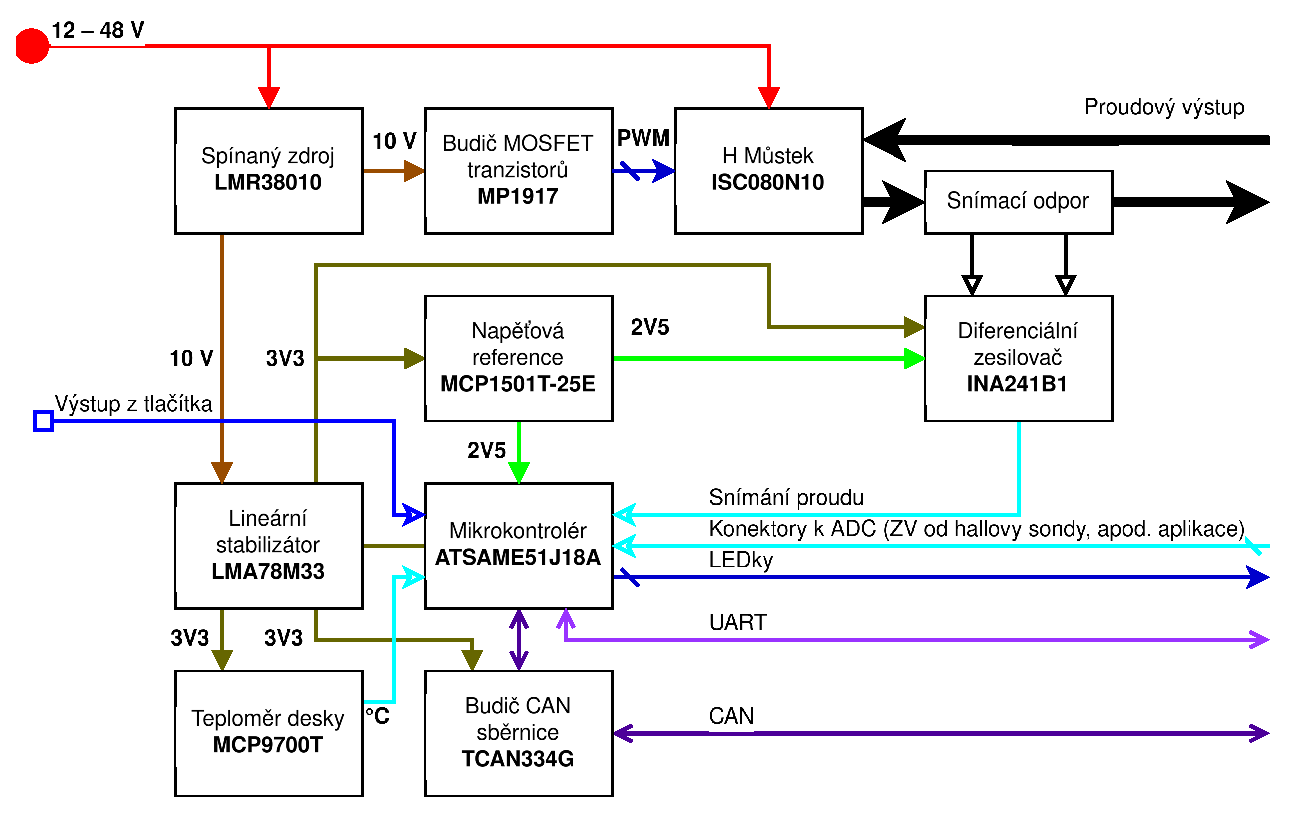
\includegraphics[width=0.9\textwidth]{kapitola2/figures/block_diagram.eps}
	\caption{Blokové schéma MoSeZ rev. B}
	\label{fig::block_diagram}
\end{figure}

\section{Vstupní obvody}

Vstupní obvody desky MoSeZ (rev. B) jsou navrženy tak,
aby zajistily spolehlivou ochranu a stabilní napájení.
Zvlnění vstupního napětí efektivně minimalizuje kombinace dvou elektrolytických kondenzátorů.
Pro ochranu proti přetížení jsou na vstupu dvě \textit{PTC} pojistky.
Jakmile proud překročí bezpečný limit, pojistky zvýší svůj odpor a odpojí napájení.
Proti přepólování je deska chráněna kombinací diody a \textit{PTC} pojistek,
zatímco varistor a \textit{TVS} dioda poskytují ochranu proti přepětí.
Měření vstupního napětí probíhá přes napěťový dělič,
který převádí maximální napětí na úroveň vhodnou pro analogově-digitální převodník mikrokontroléru.


\subsection{Vstupní elektrolytické kondenzátory}
\label{section::input_capacitors}
Minimální kapacitu vstupního kondenzátoru lze vypočítat podle jednoduchého vzorce:

\begin{equation}
	C_{\text{IN}} \geq \frac{I_{\text{LOAD}}}{f_{\text{SW}} \cdot \Delta U_{\text{ripple}}},
	\label{eq:min_capacity}
\end{equation}

kde:
\begin{itemize}
	\item $C_{\text{IN}}$ je minimální kapacita vstupního kondenzátoru ve \SI{}{\farad}
	\item $I_{\text{LOAD}}$ je proud zátěže v \SI{}{\ampere}
	\item $f_{\text{SW}}$ je spínací frekvence \SI{}{\hertz}
	\item $\Delta U_{\text{max\_zvlnění}}$ je maximální povolené zvlnění napětí \SI{}{\volt}
\end{itemize}

Maximální plánovaný výstupní proud zdroje \emph{MoSeZ} je $I_{\text{LOAD}} = \SI{8}{\ampere}$, 
ale pro rezervu ve výpočtech byl zvolen proud $I_{\text{LOAD}} = \SI{10}{\ampere}$.
Plánovaná spínací frekvence je $f_{\text{SW}} = \SI{100}{\kilo\hertz}$
a maximální přípustné zvlnění vstupního napětí bylo určeno na \SI{0,5}{\volt},
takže po dosazení do rovnice \eqref{eq:min_capacity} dostáváme:

\begin{equation}
	C_{\text{IN}} \geq \frac{10}{100 \cdot 10^3 \cdot 0,5}
\end{equation}

takže,

\begin{equation}
	C_{\text{IN}} \geq  240 \,\mu\mathrm{F}
\end{equation}

Zvolené zvlnění \SI{0,5}{\volt} zohledňuje napájecí napětí \SI{12}{\volt} a
potřebu dostatečné rezervy pro napájení pomocného spínaného zdroje \textit{LMR38010} (viz \nameref{section::smps_LMR38010}).
Tento pomocný zdroj zajišťuje výstupní napětí \SI{10}{\volt},
které je kritické pro napájení budičů \textit{MOSFET} tranzistorů \textit{MP1917}.
Napájecí napětí těchto budičů se totiž rovná spínacímu napětí na jejich výstupu (viz \cite{mp1917_ds}).
Pokud by spínací napětí MP1917 kleslo pod \SI{10}{\volt},
hrozilo by neúplné otevření hradel MOSFET tranzistorů,
což by mohlo vést k jejich přehřívání (viz \cite{ISC080N10NM6_ds}).
Vzhledem k tomu, že k významnému zvlnění dochází při vyšších výstupních proudech,
hrozí v takovém případě poškození tranzistorů vlivem tepelného průrazu.

Kvůli běžné toleranci kapacity elektrolytických kondenzátorů \SI{\pm 20}{\percent} jsem
pro filtraci napájení zvolil dvojici \SI{150}{\micro\farad} \textit{THT} kondenzátorů.
Použití \textit{THT} kondenzátorů v této kapacitní kategorii přináší finanční úsporu oproti povrchově montovaným (\textit{SMD}) kondenzátorům,
které byly použity v předchozí verzi desky \emph{MoSeZ} (rev. A).


\subsection{Nadproudová ochrana a ochrana proti přepolování}

Pro nadproudovou ochranu byly použity \textit{PTC} pojistky \textit{2920L150/60 od firmy Littelfuse}.
Oproti původnímu návrhu desky (\textit{MoSeZrev. A}) byl počet těchto pojistek snížen na dvě.
Každá z pojistek je dimenzována pro trvalý proud \SI{1,5}{\ampere},
což dohromady postačuje pro jištění trvalého proudu do \SI{3}{\ampere}.
Původní ochranná dioda byla nahrazena levnějším modelem \textit{BYG10D}.
Tato dioda spolu s \textit{PTC} pojistkami slouží jako ochrana proti přepólování.
V případě nechtěné záměny polarity napájecího napětí se dioda \textit{BYG10D} stane vodivou a zkratuje vstupní napětí.
Pokud proud z napájecího zdroje v takové situaci překročí \SI{3}{\ampere}, \textit{PTC} pojistky se zahřejí a obvod rozpojí.

V případě, kdy proud z napájecího zdroje nepřekročí prahový proud \textit{PTC} pojistek,
hrozí tepelný průraz diody \textit{BYG10D}.
To by ovšem znamenalo, že se dioda pravděpodobně stane trvale vodivou,
takže by došlo k vyřazení zdroje z provozu do doby její výměny.
Elektrolytické kondenzátory by však zůstaly ochráněny.

\section{Ochrana proti přepětí}

Pro ochranu proti přepětí na vstupu slouží kombinace varistoru a \textit{TVS} diody,
obě s pracovním napětím \SI{48}{\volt}.
Při návrhu je klíčové umístit tyto součástky co nejblíže vstupnímu konektoru.
Důležité je i jejich fyzické uspořádání od nejpomalejší po nejrychlejší,
tedy nejblíže ke vstupnímu konektoru varistor a za ním \textit{TVS} dioda.
Tím je zajištěno, že rychlá \textit{TVS} dioda omezí přepětí do doby, než se aktivuje varistor,
který následně převezme hlavní část svodového výkonu.
Varistory, jakožto pomalejší ochranné prvky, jsou schopny dlouhodobě svádět větší výkon než \textit{TVS} diody.
V případě opačného pořadí hrozí, že \textit{TVS} dioda bude muset odvést veškerý výkon,
protože na varistor, se nedostane žádné přepětí, což by mohlo vést ke zničení \textit{TVS} diody.


\subsection{Měření vstupního napětí}

Vstupní napětí je měřeno pomocí děliče napětí,
který je navržen tak, aby při \SI{48}{\volt} na vstupu dával na výstupu \SI{1,65}{\volt}.
Maximální napětí, které jsou schopny měřit AD převodníky použitého mikrokontroléru (viz \nameref{section::mcu_hw}),
je \SI{2,5}{\volt}, přičemž jsou tolerantní vůči napětí \SI{3,3}{\volt}.
To znamená, že jsou schopny měřit vstupní napětí až do \SI{106}{\volt}
a k poškození analogových vstupů MCU dojde až při napětí \SI{141}{\volt}.
Tato velká rezerva je zvolena z důvodu ochrany analogových vstupů mikrokontroléru,
a tím i jeho převodníku, před přepětím, nebo v případě, že by uživatel připojil příliš vysoké napětí.
Velikost vstupního napětí se nepoužívá pro regulaci a jeho znalost slouží pouze pro orientační měření.
Proto není kritická přesnost tohoto měření.


\section{Pomocný zdroj napětí \SI{10}{\volt}}
\label{section::smps_LMR38010}

V nové revizi \textit{DPS} zajišťuje \SI{10}{\volt} výstup pro budiče \textit{MOSFET} tranzistorů obvod \textit{LMR38010}.
Tento synchronní snižující měnič reguluje široký rozsah vstupního napětí
a minimalizuje potřebu externích ochranných součástek a
umožňuje nastavit spínací frekvenci v rozsahu \SI{200}{\kilo\hertz} až \SI{2.2}{\mega\hertz}.
Vestavěné ochrany zahrnují proudové omezení po jednotlivých cyklech,
ochranu proti zkratu a tepelnou ochranu při nadměrném vyzářeném výkonu.

\subsection{Výpočet velikosti odporů v napěťové zpětné vazbě}

Rovnice pro výpočet zpětnovazebního rezistoru z datasheetu viz \cite{mp1917_ds} říká, že

\begin{equation}
	R_{FBT} = \frac{U_{OUT} - U_{REF}}{U_{REF}} \cdot R_{FBB},
	\label{eq:lmr_fb}
\end{equation}

kde

\begin{enumerate}
	\item \(R_{FBT} \) : Odpor horního rezistoru (mezi \(U_{OUT} \) a \textit{FB} pinem), měl by vyjít v rozmezí mezi \SI{10}{\kilo\ohm} až \SI{100}{\kilo\ohm}.
	\item \(U_{OUT} \) : Požadované výstupní napětí stabilizátoru.
	\item \(U_{REF} \) : Referenční napětí, \SI{1}{\volt} pro \textit{LMR38010}.
	\item \(R_{FBB} \) : Odpor dolního rezistoru (mezi FB pinem a zemí).
\end{enumerate}

dosazením $ \quad U_{OUT} = \SI{10}{\volt}$ a $R_{FBB} = \SI{10}{\kilo\ohm}$ dostávám:

\begin{equation}
	R_{FBT} = 9 \cdot 10 \cdot 10^3 = \SI{90}{\kilo\ohm}
\end{equation}

Nicméně pro unifikaci pasivních součástek byl zvolen $ \quad R_{FBT} = \SI{100}{\kilo\ohm}$ a $R_{FBB} = \SI{10}{\kilo\ohm}$,
takže upravení rovnice \eqref{eq:lmr_fb} dostávám výstupní napětí pro tuto kombinaci, asice:

\begin{equation}
	U_{OUT} = U_{REF} \cdot \left(\frac{R_{FBT}}{R_{FBB}} + 1 \right) = 1 \cdot \left(\frac{100}{10} + 1 \right) = \SI{11}{\volt}.
	\label{eq:lmr_vout_real}
\end{equation}


Těmito \SI{11}{\volt} jsou napájeny budiče \textit{MP1917},
což znamená, že se zároveň jedná o napětí,
kterými budou budiče spínat gaty \textit{MOSFET} transistorů, viz \cite{mp1917_ds}.
Napětí \SI{11}{\volt} je dle datasheetu tranzistorů \textit{ISC080N10} přípustná velikost spínacího napětí gatů,
viz \cite{ISC080N10NM6_ds}.


\subsection{Výpočet velikosti odboru programujícího spínací kmitočet}


Rovnice pro výpočet odporu RT z datasheetu \cite{mp1917_ds} říká, že

\begin{equation}
	R_{T} = 30970 \cdot f_{SW}^{-1,027},
	\label{eq:lmr_rt}
\end{equation}

kde

\begin{enumerate}
	\item $R_{T}$ : Odpor mezi pinem textit{RT/SYNC} a zemí, udávaný v\SI{}{\kilo\ohm}.
	\item $f_{SW}$ : Spínací frekvence, udávaná v \SI{}{\kilo\hertz}.
\end{enumerate}

Pro unifikaci pasivních součástek byl zvolen R\_{T} = \SI{50}{\kilo\ohm},
respektive paralelní kombinace dvou \SI{100}{\kilo\ohm} odborů použitých v napěťové zpětné vazbě \textit{LMR38010}.
Upravením rovnice \eqref{eq:lmr_rt} dostávám skutečnou spínací frekvenci pro tuto hodnotu terminačního odporu, a sice:

\begin{equation}
	f_{SW} = \left(\frac{R_T}{30970} \right)^{-\frac{1}{1,027}} =
	\left(\frac{50}{30970} \right)^{-\frac{1}{1,027}} \approx \SI{628}{\kilo\hertz}.
	\label{eq:lmr_fsw_real}
\end{equation}

Vyšší spínací frekvence umožňují použití menších induktorů a kondenzátorů ve výstupním LC filtru,
což vede k úspoře místa a potenciálně lepší dynamické odezvě měniče.
Nicméně s rostoucí frekvencí se zvyšují ztráty způsobené parazitními kapacitami
a svody v pasivních součástkách i na plošném spoji, což může negativně ovlivnit účinnost,
zejména při nízkých výstupních výkonech.
Při velmi malých zátěžových proudech a vysokých spínacích frekvencích mohou tyto parazitní ztráty tvořit významnou část celkového výkonu,
a proto bývá výhodnější zvolit nižší spínací frekvenci, kde jsou tyto ztráty menší.
Optimální volba spínací frekvence tak závisí na kompromisu mezi velikostí pasivních součástek,
účinností a požadavky na elektromagnetickou kompatibilitu (EMI), viz \cite{buck_switching_freq_affection}


\subsection{Výpočet velikosti výstupního dolnopropustého LC filtru}

LC filtr je nezbytnou součástí každého spínaného zdroje, zejména pokud má na výstupu stejnosměrné napětí.
Pro správný výběr induktoru jsou klíčové hodnota indukčnosti a saturační proud.
Indukčnost se obvykle volí tak, aby zvlnění výstupního proudu bylo mezi \SI{20}{\percent} a \SI{40}{\percent}.

Pro výpočet minimální indukčnosti platí vztah:

\begin{equation} L \geq \frac{(U_{IN} - U_{OUT})}{f_{SW} \cdot K \cdot I_{OUT(MAX)}} \cdot \frac{U_{OUT}}{U_{IN}}. \label{eq:lmr_inductance} \end{equation}

Saturační proud induktoru by měl být alespoň tak velký jako maximální očekávaný výstupní proud, aby se zabránilo jeho nasycení.
Pro spínací frekvence nad \SI{1}{\mega\hertz} se doporučují induktory s feritovým jádrem kvůli nižším ztrátám.

Maximální výstupní proud $ I_{OUT(MAX)} $ byl zvolen \SI{0,5}{\ampere} pro zajištění dostatečné výkonové rezervy.
I přes špičkové odběry budičů se očekává, že střední hodnota výstupního proudu bude výrazně nižší.
Minimální napájecí napětí bylo stanoveno na $U_{IN} = \SI{12}{\volt}$
a požadované výstupní napětí $U_{OUT} = \SI{11}{\volt}$, viz rovnice \eqref{eq:lmr_vout_real}.
Koeficient zvlnění proudu byl zvolen $K = 0,2$ (tj. \SI{20}{\percent}) a
spínací frekvence $f_{SW} = \SI{628}{\kilo\hertz}$, viz rovnice \eqref{eq:lmr_fsw_real}.

Dosazením do rovnice \eqref{eq:lmr_inductance} dostáváme:

\begin{equation} L \geq \frac{(12 - 11)}{628 \cdot 10^3 \cdot 0,2 \cdot 0,5} \cdot \frac{11}{12} \approx \SI{29,3}{\micro\henry}. \end{equation}

Dle doporučení v datasheetu \cite{mp1917_ds} byla zvolena nejbližší vyšší vyráběná hodnota, tedy $L = \SI{33}{\micro\henry}$.

Minimální kapacita $C_{OUT}$ byla určena podle vztahu, který neuvažuje statické zvlnění,
ale zaměřuje se na schopnost zdroje reagovat na skokové změny výstupního proudu.
To je klíčové, protože zdroj bude primárně napájet budiče \textit{MOSFET} tranzistorů,
kde dochází k rychlým změnám odběru.

\begin{equation}
	C_{OUT} \geq \frac{\Delta I_{OUT}^2 \cdot L}{2 \cdot U_{OUT} \cdot U_{\text{zvlnění}}}
	\label{eq:cout_min_cap_smps}
\end{equation}

kde:

\begin{itemize}
	\item $C_{OUT}$ : Minimální kapacita výstupního kondenzátoru pro omezení překmitu napětí.
	\item $\Delta I_{OUT}$ : Maximální změna výstupního proudu v aplikaci.
	\item $L$ : Indukčnost cívky.
	\item $U_{OUT}$ : Výstupní napětí.
	\item $U_{\text{zvlnění}}$ : Maximální povolená změna výstupního napětí vlivem proudového skoku.
\end{itemize}

Pokud dosadíme následující parametry:

$\Delta I_{OUT} = \SI{1}{\ampere}, \quad
	L = \SI{33}{\micro\henry}, \quad
	U_{OUT} = \SI{11}{\volt}, \quad
	U_{\text{zvlnění}} = \SI{50}{\milli\volt}$
do rovnice \eqref{eq:cout_min_cap_smps}, dostaneme:

\begin{equation}
	C_{OUT} \geq \frac{1^2 \cdot 33 \cdot 10^{-6}}{2 \cdot 11 \cdot 50 \cdot 10^{-3}} \approx \SI{30}{\micro\farad}.
\end{equation}

Na filtraci jsou použity keramické kondenzátory s dielektrikem \textit{X7R} dimenzované na napětí \SI{25}{\volt}.
Keramika \textit{X7R} má následující vlastnosti:

\begin{itemize}
	\item \textbf{Snížení kapacity při DC napětí} – při $\frac{1}{2}$ nominálního napětí a
	      pokojové teplotě je kapacita až o \SI{30}{\percent} nižší než nominální hodnota.
	\item \textbf{Teplotní drift} – změna kapacity až $\pm15\%$ v rozsahu \SI{-50}{\degreeCelsius} až \SI{+125}{\degreeCelsius}.
	\item \textbf{Stárnutí materiálu} – kapacita klesá o jednotky procent v čase.
\end{itemize}

Vzhledem k těmto faktorům a snaze unifikovat součástky na desce \emph{MoSeZ} byla použita kombinace:

\begin{itemize}
	\item $3 \cdot \SI{22}{\micro\farad}$ keramické kondenzátory \textit{X7R}.
	\item $1 \cdot \SI{100}{\nano\farad}$ keramický kondenzátor umístěný co nejblíže k cívce pro redukci vysokofrekvenčního rušení.
\end{itemize}

Tato kombinace zajišťuje \textbf{dostatečnou rezervu kapacity}, \textbf{nižší ESR} a \textbf{lepší potlačení rušení}.

\subsection{Vstupní filtrační kondenzátory}

Na vstupu je pouze paralelní kombinace dvou \SI{22}{\nano\farad} kondenzátorů pro filtraci vysokofrekvenčního rušení.
Další kondenzátory s vyšší kapacitou byly z návrhu vyřazeny.
Důvodem je umístění obvodu \textit{LMR38010} v těsné blízkosti velkých vstupních filtračních kondenzátorů
(viz \nameref{section::input_capacitors}).
Vzhledem k této skutečnosti se ukázalo použití lokálních filtračních kondenzátorů s větší kapacitou jako zbytečné.
Toto řešení přineslo značnou prostorovou úsporu na DPS,
což bylo velmi výhodné, protože v oblasti usazení obvodu \textit{LMR38010} byl prostor velmi omezený.

\section{Pomocný zdroj napětí \SI{3,3}{\volt}}
\label{sec::linear_lm78}

Napětí \SI{3,3}{\volt} pro mikroprocesor a 
ostatní obvody jako \textit{TCAN334G}, \textit{INA241B1},
či \textit{MCP1501T}  obstarává obvod \textit{LMA78M33}.
Jedná se o lineární stabilizátor napájený \SI{10}{\volt} výstupu z \textit{LMR38010}, viz \nameref{section::smps_LMR38010}.
Filtrační kondenzátory byly zvoleny dle jasného doporučení v datasheetu bez jakýchkoliv kalkulací,
viz \cite{LM78M_ds}.
Samotý obvod je tak jednoduchý a obecně známý, že nemá cenu o něm cokoliv více psát.

V původní verzi zdroje byly pro snižování vstupního napětí použity dva snižující měniče v integrovaném obvodu \textit{MP2344}.
Tyto obvody poskytovaly napětí \SI{10}{\volt} pro napájení budičů \textit{MOSFET} tranzistorů a \SI{3,3}{\volt} pro napájení mikroprocesoru.
V důsledku náhodných přepětí na výstupu těchto obvodů docházelo k poškození mikroprocesorů.
Záměnou řešení s \textit{MP2344} se podařilo problém odstranit,i když to nemusela být vina obvodů jako takových,
ale například špatného návrhu snižujících měničů. 
Nové řešení s \textit{LM78M33} je v každém případě mnohem jednodušší a levnější.

\section{Mikrokontrolér}
\label{section::mcu_hw}

V mikrokontroléru bude implementovaný regulátor a bude obstarávat veškerou komunikaci,
včetně zpracovávání vstupů z tlačítka a rozsvicování indikačních \textit{LED}.
Nová revize využívá stejný typ mikrokontroléru, asice \textit{ATSAME51J20A}.
V původním návrhu desky byl jako zdroj kmitočtu pro mikroprocesor použit \SI{32}{\kilo\hertz} krystalový rezonátor.
Tento rezonátor způsoboval nespolehlivé spouštění při inicializaci procesoru.
V nové verzi desky byl použit \SI{20}{\mega\hertz} rezonátor, 
který byl ověřen v jiných projektech s \textit{MCU} od \textit{Microchip}.
Došlo také k opravě záměny pinů programovacího konektoru \textit{SWDIO} a \textit{SWDCLK},
což byla chyba v původním návrhu desky \textit{MoSeZ}, která vedla k výrobě specialního programovacího kabelu.

Každý digitální napájecí vstupní pin \textit{VDDIO} je odfiltrován keramickým kondenzátorem s kapacitou \SI{100}{\nano\farad}.
Ke spínanému zdroji integrovaného v mikrokontroléru je připojena indukčnost o velikosti \SI{10}{\micro\henry},
která filtruje výstupní proud a za ni je pro filtrování vzniklého napětí \textit{VDDCORE} připojena kombinace \SI{22}{\micro\farad} a \SI{100}{\nano\farad} kondenzátorů.
Analogové napětí \textit{VDDANA} se tvoří z napětí \textit{VDDIO} přes LC filtr tvořený dvěma kondenzátory a feritovou perličkou zapojenými do $\pi$ článku.
Kondenzátory mají kapacitu \SI{22}{\micro\farad} a feritová perlička o impedanci \SI{330}{\ohm} na frekvenci \SI{100}{\mega\hertz}.
Součástky byly vybrány a zapojeny dle doporučení v datasheetu, viz \cite{ATSAME51J20A_ds}.


\section{Proudový výstup}

Řízení elektromagnetických aktuátorů vyžaduje spolehlivý a výkonný proudový výstup, 
který je schopen generovat obousměrné stejnosměrné (DC) a střídavé (AC) signály s požadovanými parametry. 
Z tohoto důvodu byla v rámci proudových zdrojů \textit{MoSeZ} navržena výstupní část založená na topologii \textit{H-můstku}, 
která umožňuje obousměrný tok proudu a generování dynamicky tvarovaných průběhů.
Klíčovými aspekty návrhu výstupního obvodu jsou vhodná volba výkonových tranzistorů, 
účinné řízení spínacích prvků a tepelný management. 
V následujících podsekcích jsou rozebrány konstrukční i výpočetní aspekty této části obvodu.



\subsection{H-můstek}

Tranzistory \textit{MOSFET} původní revize desky \textit{MoSeZ} by nemohly pracovat na napětí \SI{48}{\volt}, 
proto bylo nutné zvolit nové tranzistory s parametrem \(U_{DS\_MAX} > 2 \cdot \SI{48}{\volt}\). 
Výběr padl na \textit{Infineon ISC080N10}, u kterého bylo nutné ověřit, 
že může být dlouhodobě zatěžován proudem \SI{8}{\ampere} bez rizika tepelného průrazu. 
Maximální proud do zátěže bude uvažován jako \SI{10}{\ampere}, což zajistí určitou výkonovou rezervu.

Pro výpočet celkových ztrát na \textit{MOSFET} tranzistoru se dle \cite{mosfet_losses} se používá následující vztah:

\begin{equation}
    P_{LOSS} = P_{J} + P_{SW} + P_{G}
\end{equation}

kde:

\begin{itemize}
    \item \(P_{LOSS}\): Celkové ztráty na \textit{MOSFET} tranzistoru.
    \item \(P_{J}\): Ztráty způsobené odporem kanálu \textit{MOSFET} tranzistoru (vodivostní ztráty).
    \item \(P_{SW}\): Ztráty vznikající při spínání a rozepínání tranzistoru (spínací ztráty).
    \item \(P_{G}\): Ztráty způsobené kapacitou gate tranzistoru (ztráty hradlem).
\end{itemize}

Vodivostní ztráty se vypočítají jako:

\begin{equation}
    P_{J} = I_{D}^{2} \cdot R_{DS\_ON}
    \label{eq:joullossesfet}
\end{equation}

kde ze zadání a datasheetu \cite{ISC080N10NM6_ds}:

\begin{itemize}
    \item \(I_D\): Proud protékající tranzistorem (Drain current) – \SI{10}{\ampere}.
    \item \(R_{DS\_ON}\): Odpor kanálu tranzistoru v sepnutém stavu (Drain-source resistance on-state) – \SI{8.5e-3}{\ohm}.
\end{itemize}

Dosazením těchto hodnot do rovnice \eqref{eq:joullossesfet} dostaneme:

\begin{equation}
    P_{J} = 10^2 \cdot 8.5 \cdot 10^{-3} = \SI{0,85}{\watt}
\end{equation}

Spínací ztráty se vypočítají jako:

\begin{equation}
    P_{SW} = 0,5 \cdot U_{CC} \cdot I_{D} \cdot (t_{r} + t_{f}) \cdot f_{SW}
    \label{eq:switchingFETlosses}
\end{equation}

kde dle zadání a datasheetu \cite{ISC080N10NM6_ds}:

\begin{itemize}
    \item \(U_{CC}\): Napájecí napětí – \SI{48}{\volt}.
    \item \(t_{r}\): Náběžná doba spínání – \SI{2,9e-9}{\second}.
    \item \(t_{f}\): Sestupná doba spínání – \SI{2,6e-9}{\second}.
    \item \(f_{SW}\): Spínací frekvence – \SI{100}{\kilo\hertz}.
\end{itemize}

Dosadíme tyto hodnoty do rovnice \eqref{eq:switchingFETlosses}:

\begin{equation}
    P_{SW} = 0,5 \cdot 48 \cdot 10 \cdot 2,9 \cdot 10^{-9} + 2,6 \cdot 10^{-9} \cdot 100 \cdot 10^{3} = \SI{0,1392}{\watt}
\end{equation}

Ztráty hradlem se vypočítají jako:

\begin{equation}
    P_{G} = Q_{G} \cdot U_{CC} \cdot f_{SW}
    \label{eq:FETleakgatelosses}
\end{equation}

kde dle předchozích výpočtů a datasheetu \cite{ISC080N10NM6_ds}:

\begin{itemize}
    \item \(Q_{G}\): Celkový náboj hradla (gate charge total) – \SI{2,38e-8}{\coulomb}.
\end{itemize}

Pro výše uvedené parametry, po dosazení do rovnice \eqref{eq:FETleakgatelosses} dostáváme:

\begin{equation}
    P_{G} = 2,38 \cdot 10^{-8} \cdot 48 \cdot 100 \cdot 10^{3} = \SI{0,1142}{\watt}
\end{equation}

Celkové ztráty se vypočítají jako součet všech ztrát:

\begin{equation}
    P_{LOSS} = P_{J} + P_{SW} + P_{G} = 0,85 + 0,1392 + 0,1142 = \SI{1,1034}{\watt}
\end{equation}

Maximální přípustné ztráty tranzistoru při chlazení footprintem DPS lze určit jako:

\begin{equation}
    P_{Z\_MAX} = \frac{T_{J\_MAX} - T_{\text{SURR}}}{R_{\text{thJA}}}
\end{equation}

kde dle datasheetu \cite{ISC080N10NM6_ds}:

\begin{itemize}
    \item \(T_{J\_MAX}\): Maximální přípustná teplota přechodu tranzistoru – \SI{175}{\celsius}.
    \item \(T_{\text{SURR}}\): Okolní teplota – \SI{50}{\celsius} (určeno jako teplota okolí s velkou rezervou).
    \item \(R_{\text{thJA}}\): Tepelný odpor tranzistor-okolí – \SI{75}{\kelvin\per\watt}. 
	Dle datasheetu \cite{ISC080N10NM6_ds} je \SI{50}{\kelvin\per\watt} pro \SI{6}{\centi\meter^2}. 
	Ačkoliv plánuji ještě větší chladící plochu, pro jistotu jsem přidal rezervu.
\end{itemize}

Po dosazení:

\begin{equation}
    P_{Z\_MAX} = \frac{175 - 50}{75} = \SI{1,6667}{\watt} > P_{LOSS} % Opraveno na >
\end{equation}

Takže tranzistor by neměl mít s provozem \SI{8}{\ampere} sebemenší problém. 
Teplota přechodu se při těchto provozních parametrech dá spočítat jako:

\begin{equation}
    T_{J} = T_{\text{SURR}} + P_{LOSS} \cdot R_{\text{thJA}}
\end{equation}

Po dosazení hodnot známých z předchozích výpočtů dostaneme:

\begin{equation}
    T_{J} = \SI{50}{\celsius} + \SI{1,1034}{\watt} \cdot \SI{75}{\kelvin\per\watt} = \SI{132,758}{\celsius} % Opraveno na 132,758
\end{equation}

Vypočtená teplota přechodu \SI{132,758}{\celsius} je mnohem nižší než maximální výrobcem přípustná teplota \SI{175}{\celsius}, 
takže tranzistor by měl být schopen pracovat bez rizika tepelného průrazu s relativně slušnou teplotní rezervou.
Proudový výstup je chráněn proti náhodným přepětím dvěma \textit{TVS} diododami s pracovním napětím \SI{48}{\volt},
viz \pref{priloha:schema_CurrentOutput}.


\subsection{Budiče tranzistorů}

Jsou využity dva budiče \textit{MOSFET} tranzistorů \textit{MP1917}.
Každý je řízen dvěma \textit{PWM} signály, z nichž jeden je pro řízení \textit{low-side} tranzistoru a
druhý pro řízení \textit{high-side} tranzistoru.
\textit{High-side} tranzistor je označován jako plovoucí, protože jeho \textit{Source} elektroda není přímo spojen se zemí,
ale je připojen k zátěži a \textit{low-side} tranzistoru.
Proto je výhodnější použít speciálně navržené budiče.
Pro otevření \textit{low-side} tranzistoru by stačil i napěťově zesílený signál z mikrokontroléru, což neplatí pro \textit{high-side} tranzistor.
Podmínka pro otevření libovolného \textit{MOSFET} tranzistoru je:

\begin{equation}
	U_{G} > U_{T} + U_{S}
\end{equation}

kde:

\begin{itemize}
	\item \(U_{G}\): Napětí na gate elektrodě tranzistoru.
	\item \(U_{T}\): Prahové napětí \textit{MOSFET} tranzistoru, tj. napětí při kterém se začíná otevírat (konstanta součástky).
	\item \(U_{S}\): Napětí na source elektrodě transistoru.
\end{itemize}

Pro \textit{high-side} tranzistor H-můstku platí:

\begin{equation}
	U_{GSH} > U_{T} + U_{LOAD} + U_{LS\_MOSFET}
\end{equation}

kde:

\begin{itemize}
	\item \(U_{LOAD}\): Napětí na zátěži.
	\item \(U_{LS\_MOSFET}\): Napětí na \textit{low-side} tranzistoru.
\end{itemize}

Pro plné otevření tranzistoru je nutné napětí výrazně vyšší než prahové napětí \(U_{T}\).
Tranzistory \textit{ISC080N10} jsou podle datasheetu plně otevřeny při \(U_{GS} = \SI{10}{\volt}\),
přičemž \(U_{GSMAX} = \SI{20}{\volt}\) (viz \cite{ISC080N10NM6_ds}).
Pro plné otevření tedy platí:

\begin{equation}
	U_{GSH} \ge \SI{10}{\volt} + U_{LOAD} + U_{LS\_MOSFET} < \SI{20}{\volt}
	\label{eq:mosfet_hs_opening_floatin}
\end{equation}

Napětí na zátěži \(U_{LOAD}\) a napětí na \textit{low-side} tranzistoru \(U_{LS\_MOSFET}\) jsou závislé na velikosti proudu protékajícího zátěží.
Z rovnice \eqref{eq:mosfet_hs_opening_floatin} vyplývá,
že i napětí potřebné pro otevření \textit{high-side} tranzistoru \(U_{GSH}\) se mění (plave), odtud název „plovoucí“ tranzistor.
Jednou z nejčastěji používaných metod,
jak splnit nerovnici \eqref{eq:mosfet_hs_opening_floatin},
je použití \textit{bootstrap} kondenzátoru a \textit{bootstrap} diody.

Bootstrap kondenzátor slouží jako zdroj napětí pro \textit{high-side} \textit{CMOS} budič,
který je v tomto případě integrován v \textit{MP1917}.
Kondenzátor musí být jednou elektrodou připojen přes \textit{bootstrap} diodu k napájecímu napětí budiče a
druhou elektrodou k potenciálu sourcu \textit{MOSFET} tranzistoru,
respektive k potenciálu zátěže.
Na obrázku \ref{fig::bootstrap_explained_LS_ON} je vidět,
že při sepnutí \textit{low-side} tranzistoru protéká zátěží proud \(I_{LOAD}\) a na zátěži vzniká úbytek \(U_{LOAD}\).
Zároveň je nabíjen \textit{bootstrap} kondenzátor napájecím napětím budiče,
v \oref{fig::bootstrap_explained_LS_ON} jako \(U_{DD} = \SI{10}{\volt}\),
přes \textit{bootstrap} diodu na napětí:

\begin{equation}
	U_{BSC} = \SI{10}{\volt} - U_{D} -  U_{LS} \approx \SI{10}{\volt}
	\label{eq:bootstrap_voltage_LSON}
\end{equation}

\begin{figure}[htpb]
	\centering
	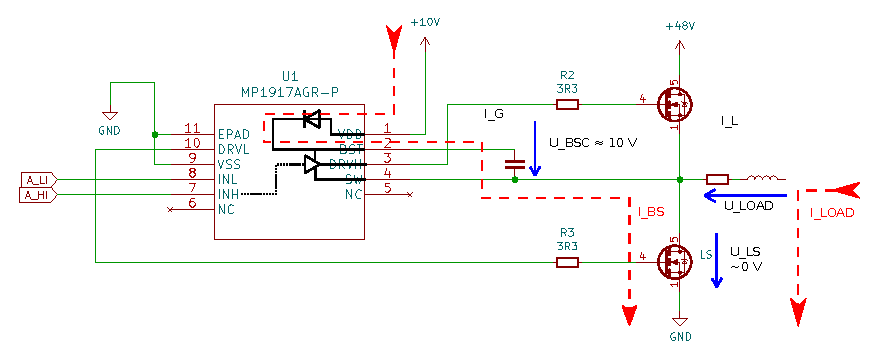
\includegraphics[width=0.9\textwidth]{kapitola2/figures/bootstrap_explained_LS_ON.eps}
	\caption{Nabíjení \textit{bootstrap} kondenzátoru přes sepnutý \textit{low-side} tranzistor na napájecí napětí budiče (\SI{10}{\volt}).}
	\label{fig::bootstrap_explained_LS_ON}
\end{figure}

Při rozepnutí tranzistoru \textit{LS} přestává být spodní elektroda kondenzátoru uzemněna a dostává se na potenciál zátěže, takže:

\begin{equation}
	U_{BSC} = \SI{10}{\volt} +  U_{LOAD}
	\label{eq:bootstrap_voltage_LSOFF} % Změněno na LSOFF pro konzistenci
\end{equation}

V tomto momentě zabraňuje vybíjení kondenzátoru \textit{bootstrap} dioda a
na \textit{bootstrap} kondenzátoru se udržuje napětí \(U_{DD} + U_{LOAD}\) vůči zemi.
Při sepnutí \textit{high-side} tranzistoru se toto napětí připojí na gate \textit{MOSFET} tranzistoru,
v \oref{fig::bootstrap_explained_LS_ON} označené jako \(U_{G}\),
a do gatu tranzistoru začne protékat vyrovnávací proud \(I_{G}\),
dokud se kapacita \(C_{G}\) nenabije na napětí \(U_{G}\). Tím je zajištěno, že

\begin{equation}
	U_{GS} = U_{BSC} \approx \SI{10}{\volt}
	\label{eq:bootstrap_voltage_lsoff} % Změněno na lsoff pro konzistenci
\end{equation}

a je dosaženo spínání \textit{high-side} tranzistoru.
Z popsaného principu je jasné, že \textit{high-side} tranzistor nemůže být spínán se střídou \SI{100}{\percent},
protože \textit{bootstrap} kondenzátor musí být nabíjen spínáním \textit{low-side} tranzistoru, viz \oref{fig::bootstrap_explained_LS_ON}.
V současnosti jsou \textit{bootstrap} diody běžně integrovány v budičích,
takže při návrhu stačí zvolit vhodný \textit{bootstrap} kondenzátor.

\begin{figure}[htpb]
	\centering
	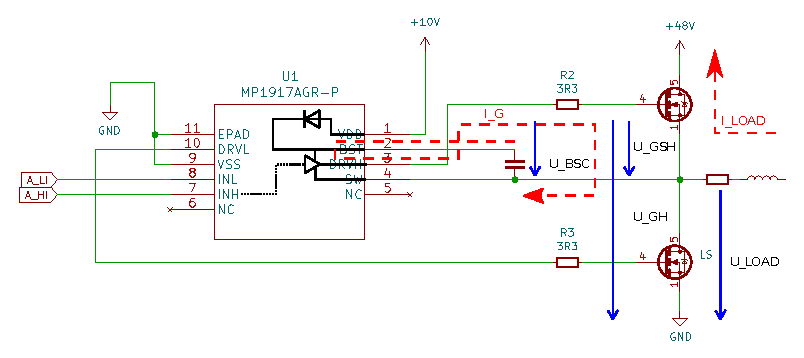
\includegraphics[width=0.9\textwidth]{kapitola2/figures/bootstrap_explained_LS_OFF.eps}
	\caption{Sepnutí \textit{high-side} tranzistoru pomocí součtu napětí na \textit{bootstrap} kondenzátoru a napětí zátěže. Směr proudu zátěží \(I_{LOAD}\) zachován z \oref{eq:bootstrap_voltage_LSON}}
	\label{fig::bootstrap_explained_LS_OFF}
\end{figure}

Tranzistory \textit{Infineon ISC080N10} mají téměř dvojnásobnou kapacitu hradla oproti původním Infineon \textit{BSZ0703L} (\emph{MoSeZ} revize A).
Proto bylo nutné přepočítat hodnoty \textit{bootstrap} kondenzátorů pro budiče \textit{MP1917}.
Výpočet minimální kapacity \textit{bootstrap} kondenzátoru \(C_{\textit{bootstrap}}\) se provádí pomocí provnic \eqref{eq:cboot_min_cap} až \eqref{eq:delta_uhs}
převzatých z \cite{bootstrap_moudra}:

\begin{equation}
	C_{\textit{bootstrap}} \geq \frac{Q_{total}}{\Delta U_{BSTQ}}
	\label{eq:cboot_min_cap}
\end{equation}

kde:

\begin{itemize}
	\item \(C_{\textit{bootstrap}}\): Minimální požadovaná kapacita \textit{bootstrap} kondenzátoru.
	\item \(Q_{total}\): Celkový náboj potřebný pro nabití a udržení hradla \textit{MOSFET} tranzistoru v otevřeném stavu.
	\item \(\Delta U_{BSTQ}\): Maximální přípustný pokles napětí na \textit{bootstrap} kondenzátoru během spínacího cyklu.
\end{itemize}

Celkový náboj \(Q_{total}\) se vypočítá podle vztahu:

\begin{equation}
	Q_{total} = Q_G + I_{DDQ} \cdot \frac{D_{max}}{f_{sw}} + I_{BSTQ} \cdot \frac{1-D_{max}}{f_{sw}}
	\label{eq:qtotal}
\end{equation}

kde:

\begin{itemize}
	\item \(Q_G\): Celkový náboj hradla vybraného \textit{MOSFET} tranzistoru.
	\item \(I_{DDQ}\): Klidový (svodový) proud \textit{\textit{high-side}} budiče.
	\item \(I_{BSTQ}\): Klidový (svodový) proud \textit{bootstrap} obvodu budiče.
	\item \(D_{max}\): Maximální střída \textit{PWM} signálu,
	      v desetiném vyjádření (např. 0.985 pro \SI{98.5}{\percent}).
	\item \(f_{sw}\): Spínací frekvence \textit{PWM} signálu.
\end{itemize}


Dosazením konkrétních hodnot z datasheetu \cite{mp1917_ds}:
\(Q_G = \SI{19}{\nano\coulomb}\),
\(I_{DDQ} = \SI{150}{\micro\ampere}\),
\(I_{BSTQ} = \SI{90}{\micro\ampere}\),
\(D_{max} = 0.985\), \(f_{sw} = \SI{100}{\kilo\hertz}\),
lze vypočíst hodnotu celkového \(Q_{total}\) dle rovnice \eqref{eq:qtotal} jako:


takže

\begin{equation}
	Q_{total} = 19 \cdot 10^{-9} + 150 \cdot 10^{-6} \cdot \frac{0,985}{100 \cdot 10^{3}} + 
	90 \cdot 10^{-6} \cdot \frac{1-0,985}{100 \cdot 10^{3}} \approx \SI{20,48}{\nano\coulomb},
\end{equation}

Maximální přípustný pokles napětí na \textit{bootstrap} kondenzátoru \(\Delta V_{BSTQ}\) se určí z rovnice:

\begin{equation}
	\Delta V_{BSTQ} = U_{DD} - U_{DH} - U_{UPFT} = U_{DD} - U_{DH} - U_{UPRT} - U_{HT}
	\label{eq:delta_uhs}
\end{equation}

kde:

\begin{itemize}
	\item \(U_{DD}\): Napájecí napětí budiče hradla \textit{IC}.
	\item \(U_{DH}\): Úbytek napětí na \textit{bootstrap} diodě.
	\item \(U_{UPFT}\): Prahová hodnota podpěťové ochrany budiče při poklesu napětí na napájecím pinu.
	\item \(U_{UPRT}\): Prahová hodnota podpěťové ochrany budiče při náběhu napětí na napájecím pinu.
	\item \(U_{HT}\): Hystereze podpěťové ochrany budiče.
\end{itemize}

Dosazením konkrétních hodnot z datasheetu \cite{mp1917_ds}:
\(U_{DD} = \SI{11}{\volt}\),
\(U_{DH} = \SI{0,95}{\volt}\),
\(U_{UPRT} = \SI{7,2}{\volt}\),
\(U_{HT} = \SI{0,5}{\volt}\),
lze vypočíst hodnotu celkového \(U_{BSTQ}\) dle rovnice \eqref{eq:delta_uhs} jako:

\begin{equation}
	\Delta U_{BSTQ} = 11 - 0,95 - 7,2 - 0,5 = \SI{2,35}{\volt}.
\end{equation}

Výpočet minimální kapacity \textit{bootstrap} kondenzátoru \(C_{\textit{bootstrap}}\) dle rovnice \eqref{eq:cboot_min_cap}:

\begin{equation}
	C_{\textit{bootstrap}} \geq \frac{\SI{20,48}{\nano\coulomb}}{\SI{2,35}{\volt}} \approx \SI{8,71}{\nano\farad}.
\end{equation}

Pro zajištění dostatečné funkční rezervy byl v obvodu zvolen \textit{bootstrap} kondenzátor s kapacitou \SI{22}{\nano\farad}.
Je však důležité poznamenat, že volba příliš vysoké kapacity \textit{bootstrap} kondenzátoru není žádoucí.
S rostoucí kapacitou se totiž zvyšuje náchylnost k oscilacím na hradle tranzistorů během spínání a rozpínání,
což je způsobeno vznikem rezonancí s parazitními indukčnostmi v budicím obvodu, viz \cite{bootstrap_moudra}.

Naopak, nedostatečná kapacita \textit{bootstrap} kondenzátoru by mohla vést k neúplnému otevření hradla tranzistoru,
a tím ke zvýšení jeho spínacího odporu a ztrátového výkonu.
Zvýšené ztráty by se mohly projevit nepřijatelným zahříváním tranzistorů a potenciálně i jejich poškozením tepelným průrazem.
Pro potlačení oscilací na hradle tranzistoru se doporučuje zařadit tlumící odpor sériově mezi výstup budiče a hradlo tranzistoru.
Tlumící účinek rezistoru se zvyšuje s jeho odporem,
nicméně příliš vysoká hodnota tlumícího odporu zpomaluje nabíjení a vybíjení hradla,
prodlužuje spínací časy a opětovně zvyšuje spínací ztráty.


\section{Měření výstupního proudu}
\label{section::current_meassure}

Pro měření proudu je použit integrovaný obvod \textit{INA241},
což je vysoce přesný obousměrný senzor proudu s pevně nastaveným zesílením.
Tento senzor umožňuje měřit úbytek napětí na snímacích rezistorech v širokém rozsahu souhlasného napětí,
konkrétně od \SI{-5}{\volt} do \SI{110}{\volt},
a to zcela nezávisle na napájecím napětí obvodu.

Vysoká přesnost měření je u obvodu \textit{INA241} zajištěna zejména nízkým vstupním offsetem,
který dosahuje maximálně \SI{\pm10}{\micro\volt},
vysokým poměrem potlačení souhlasného signálu (\textit{CMRR}) pro stejnosměrný proud, typicky \SI{166}{\decibel},
a efektivní schopností potlačení rušení \textit{PWM} signálem díky speciální vnitřní konstrukci,
která by měla minimalizovat přenos rušení, generovaného spínáním tranzistorů, na vstup měřicího obvodu.


\subsection{Napěťová reference}
\label{section::voltage_ref}

Obvod \textit{INA241B1} umožňuje použití vnitřního nebo vnějšího referenčního napětí.
Vnitřní referenční zdroj se aktivuje ponecháním pinů \textit{REF1} a \textit{REF2} nezapojených.
V tomto režimu je výstupní napětí při nulovém proudu rovno polovině napájecího napětí,
což znamená, že výstup je přirozeně ratiometrický – jeho hodnota se mění v závislosti na napájecím napětí.

Bohužel, AD převodníky integrované v mikrokontroléru \textit{ATSAME51J20A} se
dostávají do saturace při napětích vyšších než \SI{2,5}{\volt},
což omezuje využití plného rozsahu výstupu obvodu \textit{INA241B1} při použití vnitřní reference.
Z tohoto důvodu bylo zvoleno zapojení s externí referencí, kde
\textit{REF1} je připojen na výstup přesné napěťové reference a \textit{REF2} je uzemněn.
Tím se výstupní napětí při nulovém proudu posouvá na polovinu napětí referenčního zdroje.
Použitím externí referenční napěťové reference \textit{MCP1501T-25E} s hodnotou \SI{2.5}{\volt}
je pracovní bod výstupu nastaven na \SI{1.25}{\volt} při nulovém vstupním proudu.

Pokud je stejné referenční napětí \SI{2.5}{\volt} použito jako referenční vstup pro AD převodník mikrokontroléru,
je opět zajištěn ratiometrický převod.
To znamená, že výstupní napětí zesilovače i referenční napětí AD převodníku jsou vzájemně proporcionální ke stejnému zdroji,
čímž se eliminuje vliv kolísání napájecího napětí na výsledek měření.

\subsection{Snímací rezistor}

Při výpočtu snímacího rezistoru měření proudu vycházíme z maximálního proudu zátěží,
\(I_{\text{LOAD\_MAX}}\), který je specifikován v zadání úlohy jako \SI{10}{\ampere}.
Dále je nezbytné definovat maximální přípustný výkon, \(P_{D\_MAX}\),
který se bude vyzařovat na snímacím rezistoru.
Obecně platí, že s rostoucím odporem snímacího rezistoru klesají nároky na zesílení zesilovače,
což typicky vede k vyšší přesnosti měření.
Hlavní nevýhodou většího odporu je však nárůst ztrátového výkonu,
který se musí vyzářit, což má negativní dopad na celkovou účinnost systému.

Předpokládejme, že maximální přípustný ztrátový výkon je stanoven na \(P_{D\_MAX} = \SI{0,5}{\watt}\).
Tato hodnota představuje rozumný kompromis, kdy vyzářené teplo lze ještě efektivně odvádět.
V dalším kroku určíme maximální přípustnou velikost snímacího rezistoru, \(R_{\text{SENSE}_\text{MAX}}\), z hlediska ztrátového výkonu:

\begin{equation}
	\label{eq::eq_rsense_maxR}
	R_{\text{SENSE\_PMAX}} = \frac{P_{D\_MAX}}{I_{\text{LOAD\_MAX}}} = \frac{0,5}{10} = \SI{50}{\milli\ohm},
\end{equation}

Pak je nutné zvolit odpor, jehož velikost bude menší než \(R_{\text{SENSE}\_MAX}\)
a který v kombinaci se zesílením \(G\) plně využije dynamický rozsah následujících obvodů.
V tomto konkrétním případě následuje \textit{AD} převodník integrovaný v mikrokontroléru s rozsahem \SI{0}{\volt} až \SI{2,5}{\volt}.
Pro nulový proud je však výstupní napětí zesilovače \textit{INA241} (\(U_{OUT}\)) nastaveno na \SI{1,25}{\volt}
díky napěťové referenci \(U_{REF}\) (viz \nameref{section::voltage_ref}).
Efektivní napěťový rozsah pro měření proudu v jednom směru je tedy \(U_{RANGE} = \SI{1.25}{\volt}\).
Obvod \textit{INA241} se vyrábí s různými zesíleními \(G\). Pro úvodní výpočet zvolíme nejmenší dostupné zesílení, a to \(G = 10 \cdot\).

\begin{equation}
	\label{eq::eq_rsense_maxURANGE}
	R_{\text{SENSE\_UMAX}} = \frac{U_{RANGE}}{I_{\text{LOAD\_MAX}} \cdot G} = \frac{1,25}{10 \cdot 10} = \SI{12,5}{\milli\ohm},
\end{equation}

Pokud nepplatí, že:

\begin{equation}
	\label{eq::eq_rsense_check_PMAX}
	R_{\text{SENSE\_UMAX}} \le R_{\text{SENSE\_PMAX}},
\end{equation}

je nutné přistoupit k úpravě návrhu.
Jednou z možností je volba zesilovače s větším zesílením \(G\).
Alternativně lze zvážit i navýšení maximálního přípustného ztrátového výkonu \(P_{D\_MAX}\).
V tomto konkrétním případě však nerovnice \eqref{eq::eq_rsense_check_PMAX} platí s dostatečnou rezervou ztrátového výkonu.
Proto postačí nalézt nejbližší menší standardně vyráběný snímací odpor, kterým je v tomto případě \SI{12}{\milli\ohm}.

Po zvolení odporu \(R_{SENSE} = \SI{12}{\milli\ohm}\) je klíčové vypočítat citlivost měření proudu v jednotkách \SI{}{\volt/\ampere}.
Znalost citlivosti je nezbytná pro následný výpočet aktuálního proudu z naměřeného výstupního napětí na obvodu \textit{INA241B1},
respektive z napětí na \textit{AD} převodníku mikrokontroléru.
Tuto citlivost lze stanovit z rovnice:

\begin{equation}
	\label{eq::sensitivity_INA}
	\text{Citlivost} = \frac{U_{RANGE}}{I_{\text{LOAD\_MAX}}} = \frac{1,25}{10} = \SI{0,125}{\volt/\ampere}.
\end{equation}

takže

\begin{equation}
	\label{eq::sensitivity_INA_val}
	Citlivost = \SI{0,12}{\volt/\ampere},
\end{equation}

\subsection{Filtrování napětí na snímacím odporu}

Pro eliminaci nežádoucího rušení v měřeném napětí na snímacím rezistoru \(R_{SENSE}\) se v obvodu používají dva typy dolnopropustných filtrů:

\begin{enumerate}
	\item \textit{Common-mode} filtr – Tento typ filtru je určen k potlačení rušení,
	      které je společné pro oba vstupy měřicího obvodu.
	      Jinými slovy, potlačuje rušení, které se na obou vstupech objevuje ve stejné fázi.
	      Hlavními zdroji rušení jsou kapacitní vazba mezi spínacími tranzistory H-můstku a zemí,
	      elektromagnetické rušení (EMI) a nekvalitní zemnění.
	\item \textit{Differential-mode} filtr – Tento typ filtru slouží k potlačení rušení,
	      které se projevuje jako rozdíl mezi napětími na obou vstupech měřicího obvodu.
	      Toto rušení se na obou vstupech objevuje se stejnou amplitudou, avšak v opačné fázi.
	      Hlavním zdrojem jsou rychlé změny proudu při spínání tranzistorů H-můstku,
	      které způsobují napěťové přechody na tomto snímacím rezistoru.
\end{enumerate}

Zlomová frekvence \textit{Common-mode} filtru, označená \(f_{CM}\), se vypočítá dle následujícího vztahu:

\begin{equation}
	f_{CM} = \frac{1}{2 \pi R_{CM} C_{CM}}
\end{equation}

kde:

\begin{itemize}
	\item \(f_{CM}\): Zlomová frekvence \textit{Common-mode} filtru.
	\item \(R_{CM}\): Hodnota odporu použitého v \textit{Common-mode} filtru.
	\item \(C_{CM}\): Hodnota kapacity použitého v \textit{Common-mode} filtru.
\end{itemize}

Pro hodnoty součástek \(R_{CM} = \SI{2.2}{\kilo\ohm}\) a \(C_{CM} = \SI{1}{\nano\farad}\) získáme:

\begin{equation}
	f_{CM} = \frac{1}{2 \pi \cdot \SI{2.2}{\kilo\ohm} \cdot \SI{1}{\nano\farad}} \approx \SI{72}{\kilo\hertz}.
\end{equation}

Vzhledem k charakteru rušení je nezbytné aplikovat \textit{Common-mode}
filtr na oba vodiče vedoucí od snímacího rezistoru.
Schéma zapojení filtru je detailněji znázorněno v \pref{priloha:schema_CurrentOutput}.

Zlomová frekvence \textit{Differential-mode} filtru, označená \(f_{DM}\), se vypočítá dle následujícího vztahu:

\begin{equation}
	f_{DM} = \frac{1}{2 \pi R_{DM} C_{DM}} =  \frac{1}{2 \pi (2 \cdot R_{CM}) C_{DM}}
\end{equation}

kde:

\begin{itemize}
	\item \(f_{DM}\): Zlomová frekvence \textit{Differential-mode} filtru.
	\item \(R_{DM}\): Hodnota odporu použitého v \textit{Differential-mode} filtru. V zapojení, kde odpory \(R_{CM}\) tvoří část \textit{Differential-mode} filtru, je \(R_{DM}\)  paralelní kombinací \(R_{CM} || R_{CM} = \frac{R_{CM}}{2}\).
	\item \(C_{DM}\): Hodnota kapacity použitého v \textit{Differential-mode} filtru.
\end{itemize}

Pro hodnoty součástek \(R_{DM} = \SI{4.4}{\kilo\ohm}\) a \(C_{DM} = \SI{1}{\nano\farad}\) dostaneme:

\begin{equation}
	f_{DM} = \frac{1}{2 \pi \cdot \SI{4.4}{\kilo\ohm} \cdot \SI{1}{\nano\farad}} \approx \SI{36}{\kilo\hertz}.
\end{equation}

\begin{figure}[htpb]
	\centering
	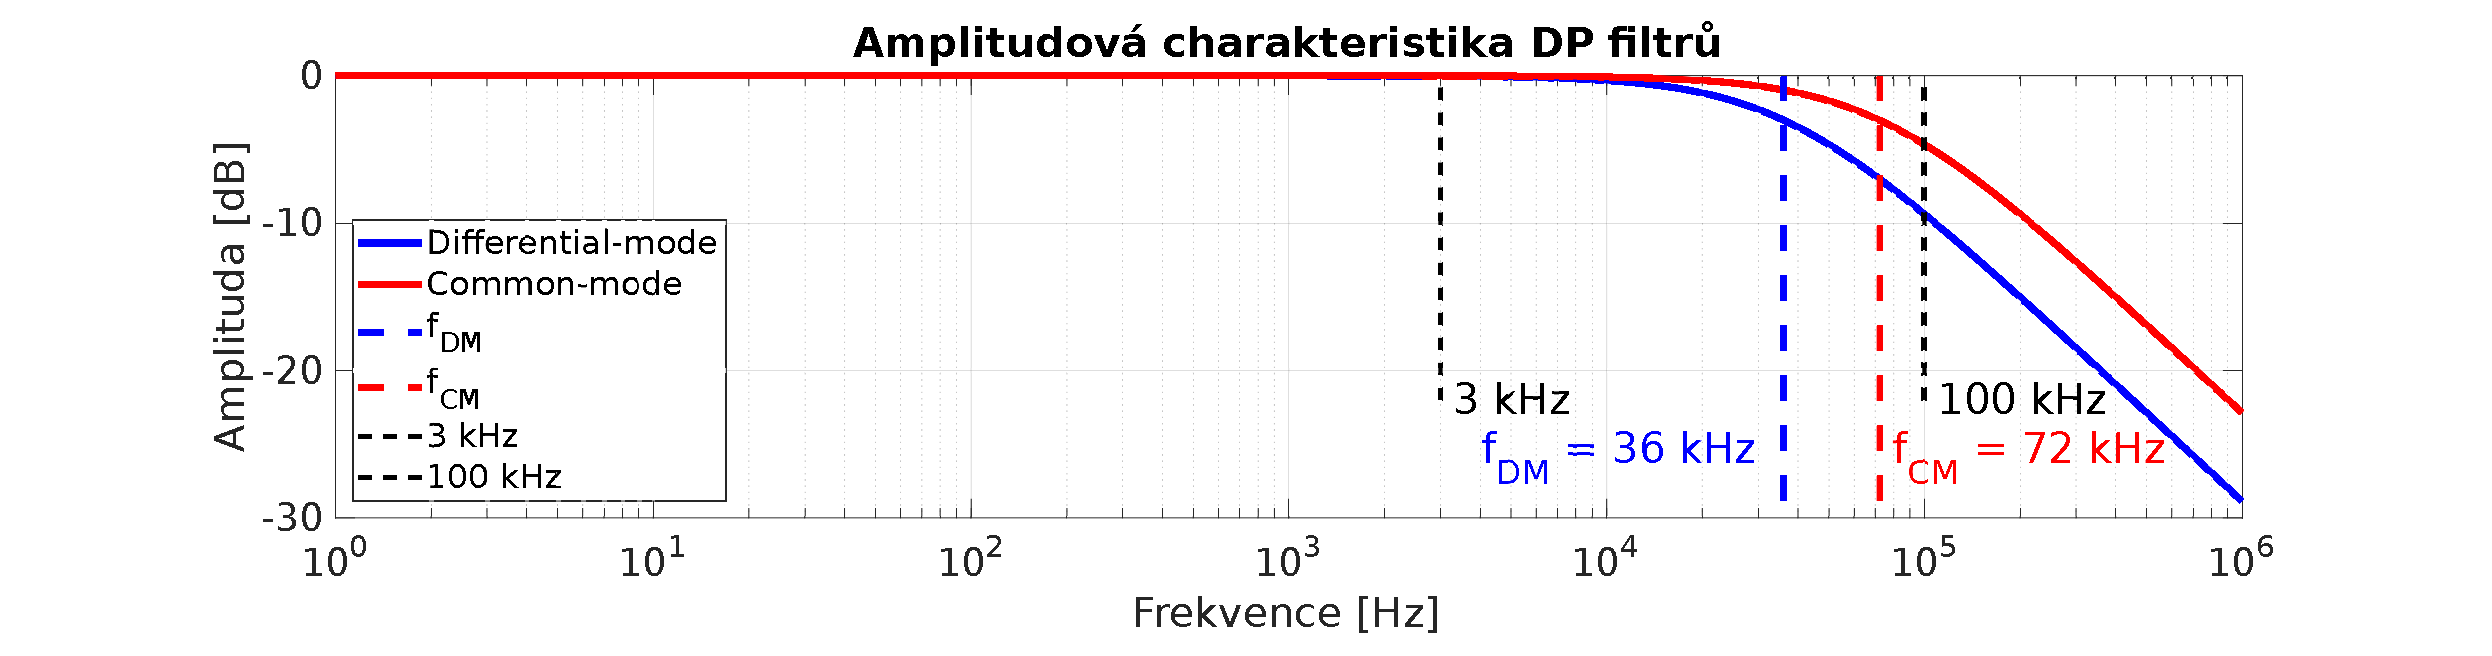
\includegraphics[width=0.9\textwidth]{kapitola2/figures/filter_f_char.eps}
	\caption{Útlumové charakteristiky pro dolnopropustné filtry prvního řádu \textit{CM} a \textit{DM} připojené mezi diferenciální zesilovač \textit{INA241B1} a snímací odpor}
	\label{fig::LP_filtter}
\end{figure}


Frekvence užitečného signálu by měla být menší než  \(\frac{1}{10}\) nejnižší mezní frekvence z obou filtrů.
To je jeden z důvodů, proč je v řešení \nameref{section::dds_implementation} maximální nastavitelná frekvence výstupního proudu stanovena na \SI{3}{\kilo\hertz}, 
vyznačená v amplitudové charakteristice na \oref{fig::LP_filtter}.
Maximální reálná frekvence bude ovlivněna indukčností zátěže.

\section{CAN Bus Driver}
\label{section::CAN_Bus_Driver}

Při vedení vodivých cest pro \textit{CAN bus} byly využity diferenciální páry s řízenou diferenciální impedancí o velikosti \SI{120}{\ohm}. 
Každá deska má dva možné způsoby připojení ke sběrnici \textit{CAN}. 
První je přes \textit{\textit{THT} pass throug header}, 
kde se desky skládáním do sebe automaticky připojí k \textit{CAN} sběrnici, viz zelený rámeček v \oref{fig::CAN_connector}. 
Druhou možností jsou dva konektory, kde jeden slouží jako vstup a druhý jako výstup \textit{CAN} sběrnice, viz bílý rámeček v \oref{fig::CAN_connector}. 
Vzhledem k tomu, že sběrnice vzniká skládáním desek, je důležité vyřešit její terminaci.


\begin{figure}[htpb]
	\centering
	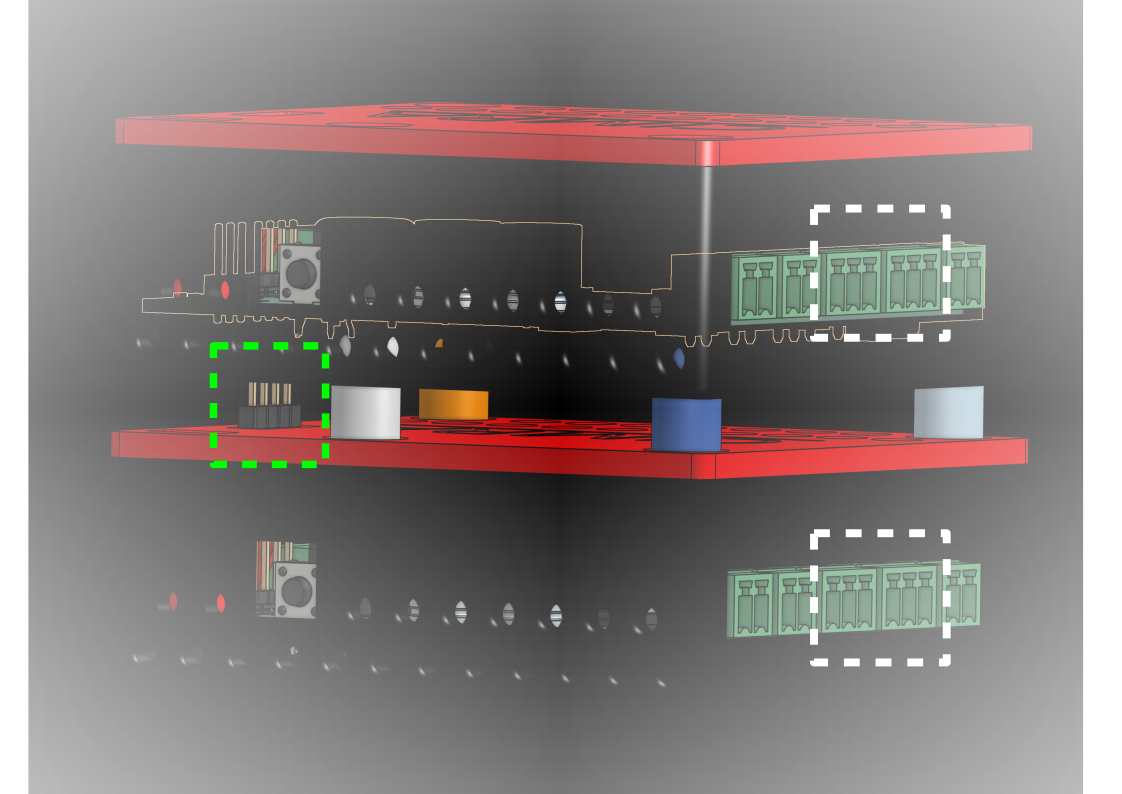
\includegraphics[width=0.9\textwidth]{kapitola2/figures/can_connector.png}
	\caption{Možnosti připojení ke \textit{CAN} sběrnici, \textbf{zelený} rámeček \textit{\textit{THT} pass throug header}, přes konektory v  \textbf{bílém} rámečku}
	\label{fig::CAN_connector}
\end{figure}	


Na desce nejsou přítomny žádné terminační odpory, a to z toho důvodu, že terminační odpory by měly být přítomny pouze na začátku a 
konci sběrnice.
Vzhledem ke konstrukci, kdy sběrnice vzniká skládáním desek, 
by terminační odpor měla obsahovat pouze první a poslední deska na sběrnici. 
Aby mohly být všechny desky plošných spojů stejné, tj. bez vytváření dedikovaných terminačních desek \textit{MoSeZ}, 
respektive desek, které mají terminační odpory připájené, bylo rozhodnuto, že terminační odpory se budou na první a 
poslední desku připojovat do jednoho z \textit{CAN} konektorů, viz bílý rámeček v \oref{fig::CAN_connector}.


\section{Interface}

Každý ze vstupů je chráněn \textit{TVS} diodami proti přepětím, 
zejména proti \textit{ESD}.
Pro zajištění dobré funkce \textit{TVS} diod je nutné je umístit co nejblíže ke konektorům a headerům.
V nové revizi je možnost měřit až dva analogové signály s rozsahem \SIrange{0}{2,5}{\volt} připojené k desce.
Hlavním záměrem je možnost zavedení informace o stavu aktuátorů do zpětné vazby regulátoru.
Toho se v této práci využívá při sledování polohy jádra voicecoilu pomocí vhodně umístěného hallova senzoru, viz \nameref{sec::voicecoil_function}.
Ovšem lze tyto vstupy využít pro měření libovolného analogového napětí v rozsahu \SI{3,3}{\volt}.

Ze staré revize zůstávají dva napájecí dvoupinové konektory, dva \textit{CAN} třípinové konektory, 
jeden dvoupinový konektor pro proudový výstup, 
třípinový header pro komunikaci přes \textit{UART} a jeden čtyřpinový header pro rozvod \textit{CAN} a napětí \SI{3,3}{\volt}.

\begin{figure}[htpb]
    \centering
    \includegraphics[width=0.9\textwidth]{kapitola1/figures/pcb_fornt.jpg}
    \caption{Přední strana DPS MoSeZ rev. B, zadní strana DPS viz příloha A: \nameref{priloha:pcb_back}}
    \label{fig::mosez_pcb_front}
\end{figure}


\newpage

\chapter{3D tisk}

Pro novou revizi desky byla navržena a vytištěna ochranná krabička, 
osazovací podložka a přípravek pro aplikaci pájecí pasty. 
Tyto prvky umožňují efektivní montáž, ochranu a zlepšení procesu výroby DPS. 

Konstrukce byla navržena pomocí online CAD softwaru \emph{Onshape}, 
což umožnilo rychlé iterace návrhu a snadné sdílení modelů.
 Výroba proběhla na \textit{3D} tiskárně \emph{Prusa Mk4}, 
 případně na jiném dostupném modelu tiskárny značky \emph{Prusa}. 

Všechny tištěné součásti využívají výplň \SI{15}{\percent} se vzorem \textit{3D Honeycomb}, 
která poskytuje optimální kombinaci pevnosti a úspory materiálu. 
Kromě toho byly aplikovány minimálně dva vnější vertikální perimetry 
a pět plných horizontálních vrstev na spodní straně, 
zatímco horní strana obsahuje čtyři plné vrstvy.
 Jako materiál byl zvolen \textit{PETG}, 
 který nabízí výbornou mechanickou odolnost, 
 tepelnou stabilitu a zároveň je vhodný pro ap	likace vyžadující pevnost a pružnost.

\section{Krabička}
Pro ochranu nové \textit{DPS}, bylo potřeba navrhnout krabičku s odnímatelným víkem.
Víko drží na krabičce pouze třením, to znamená bez použití zámků nebo šroubů.
Uvnitř krabičky se nachází 4 distanční sloupky, do kterých byly zataveny mosazné závity,
které umožňují spolehlivou, a opakovanou, montáž, či demontáž, DPS. 
Z boku a na víku krabičky jsou umístěny větrací otvory.
Jejich umístění a velikost byly zvoleny tak, aby se vzduch v krabičce pohyboval předvídatelným směrem.
Jinými slovy byla snaha o vytvoření airflow uvnitř krabičky a tím došlo ke vzniku optimálního chlazení.
Spodní řáda děr nacházejících se zboku krabičky by měla sloužit pro nasávání vzduchu pro chlazení spodní části desky MoSeZ.
Nasáty vzduch pak putuje kolem součástek na spodní straně DPS a ohřátý opouští krabičku otvory ve víčku.

\begin{figure}[H]
	\centering
	\includegraphics[width=0.75\linewidth]{kapitola3/figures/boxes_front.pdf}
	\caption{Krabičky pro MoSeZ}
	\label{priloha:boxes_front}
\end{figure}

\section{Osazovací podložka a přípravek pro aplikaci pájecí pasty}

Pro osazení byla využita automatická osazovačka \emph{OpenPnP}.
Osazovací automat vyžaduje, aby horní vrstva DPS byla ve výšce \SI{10}{\milli\meter} od pracovní desky. 
Návrh podložky tedy zohledňuje tloušťku samotné DPS a potřebnou výšku, aby osazování probíhalo správně. 
Podložka je pevně připevněna k pracovní desce osazovacího automatu 
a DPS se k ní uchycuje přes její montážní otvory.

\begin{figure}[H]
	\centering
	\includegraphics[width=0.75\linewidth]{kapitola3/figures/pap_holder.pdf}
	\caption{Držák DPS pro osazovačku}
	\label{priloha:pap_holder}
\end{figure}


Ke snadné aplikaci pájecí pasty byl navrhnut přípravek,
do kterého se upevní DPS a přes něj šablona.
Při aplikaci se šablona přitlačí na DPS 
a pomocí stěrky se nanese tenká vrstva pájecí pasty přes otvory v šabloně. 
Díky tomu je zajištěno, že pasta je aplikována pouze na pájecí plochy, 
čímž se minimalizuje riziko nežádoucích spojů a usnadňuje proces reflow pájení.

\begin{figure}[H]
	\centering
	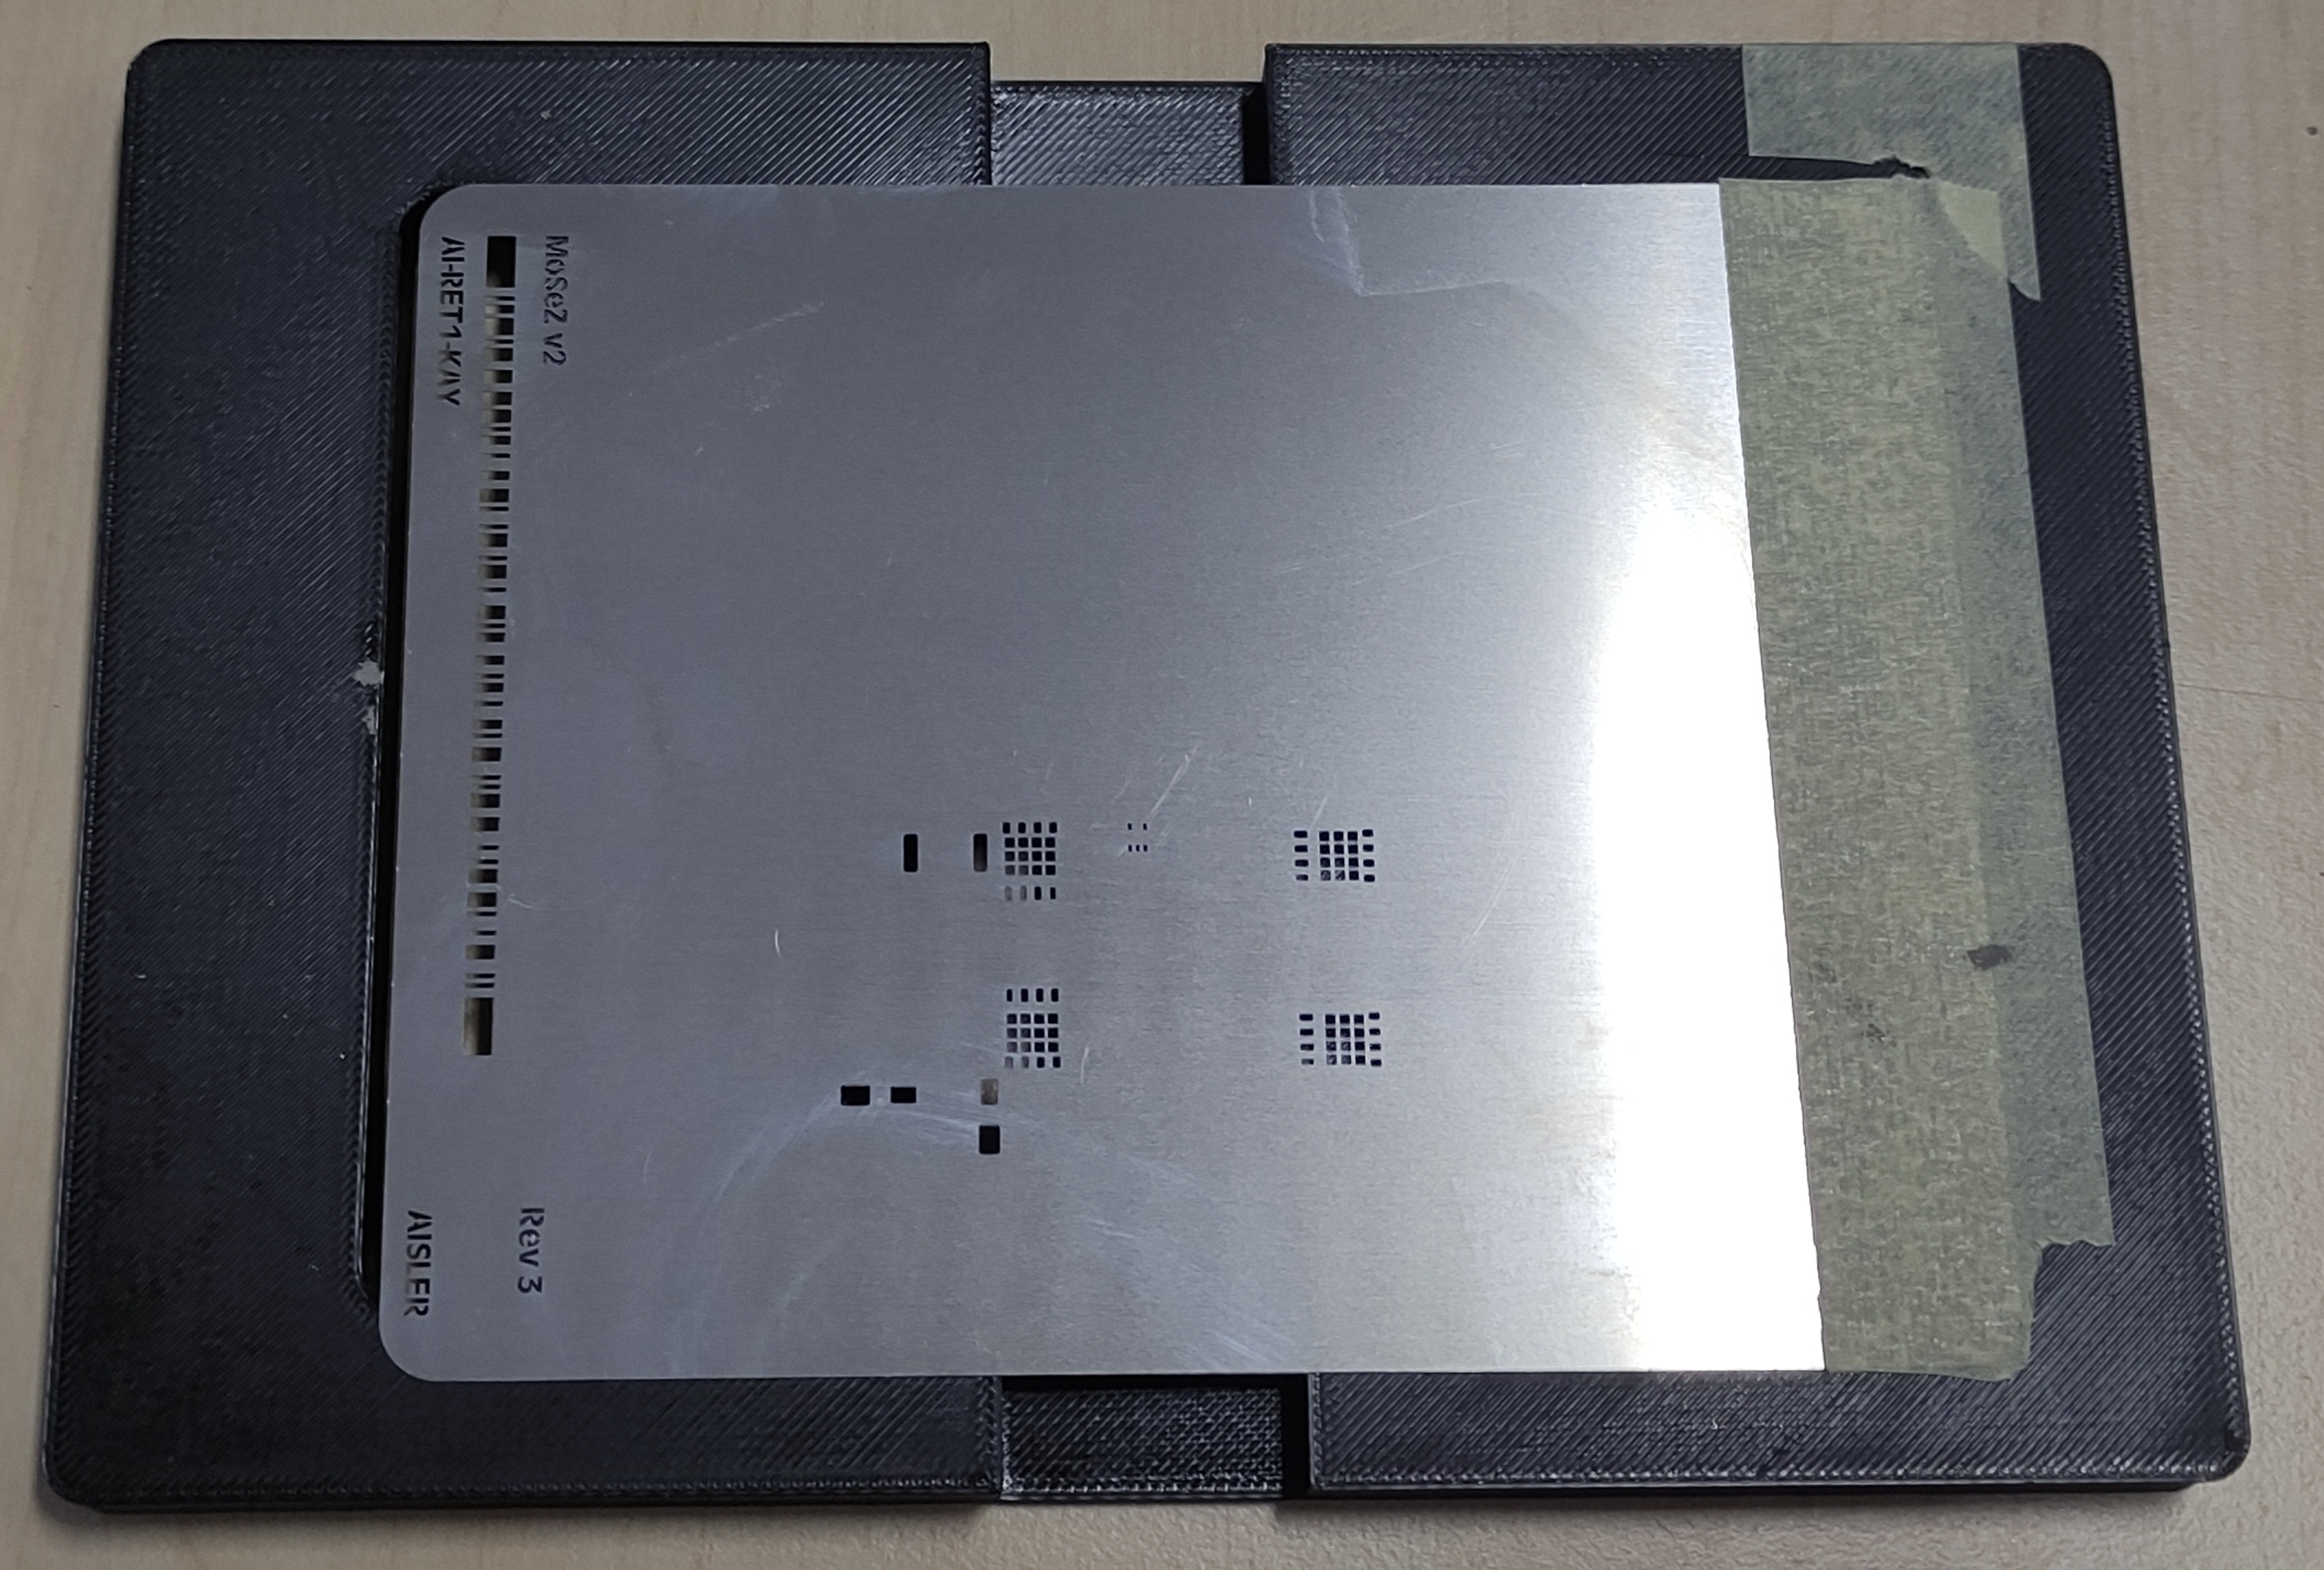
\includegraphics[width=\linewidth]{kapitola3/figures/paste_back.pdf}
	\caption{Držák DPS pro aplikaci pájecí pasty na zadní stranu DPS s již připevněnou šablonou}
	\label{priloha:paste_holder}
\end{figure}

\newpage

\chapter{\textit{Firmware} ARON}

Kapitola je rozčleněna do několika sekcí,
které popisují hlavní funkce \textit{firmwaru} a jeho implementaci.
Každá sekce se zaměřuje na konkrétní oblasti, které jsou klíčové pro správný chod systému.
Struktura kapitol zhruba odpovídá hlavním třídám, jež se v \textit{\textit{firmwaru}} nacházejí.
Začínáme základním nastavením mikrokontroléru, které je nezbytné pro inicializaci celého systému,
pokračujeme přes popis komunikačních protokolů, implementaci regulátorů, metody řízení
až po hlavní smyčku a obslužná přerušení.


\section{Nastavení systému}
\label{section::System_settings}
Tato sekce popisuje základní nastavení mikrokontroléru a jeho inicializaci,
která je obsažena v souboru \texttt{system\_settings.hpp}.


\subsection{Konfigurace hodin}
Nejprve je nakonfigurován systém hodin.
Jako zdroj hodinového signálu GCLK2 je použit externí krystal s frekvencí \SI{20}{\mega\hertz}.
Tento signál je předdělen na \SI{1}{\mega\hertz} a použit jako GCLK1,
což usnadňuje další násobení ve dvou fázových závěsech (\texttt{DPLLx}).

\begin{figure}[htbp]
	\centering
	\includegraphics[width=0.9\textwidth]{kapitola4/figures/gclk_fig.png}
	\caption{Rozvod hodin \textit{GCLK} v mikrokontroléru \texttt{ATSAME51J20A} (převzato z \cite{ATSAME51J20A_ds}, s. 139)}
	\label{fig:Datasheet_gclk}
\end{figure}

\begin{itemize}
	\item Výstup z prvního fázového závěsu \texttt{DPLL1} poskytuje \SI{120}{\mega\hertz} jako GCLK0,
	      který slouží jako hlavní systémové hodiny a je využíván ve všech periferiích,
	      pokud není uvedeno jinak.
	\item Dělením frekvence GCLK0 vzniká GCLK3 s hodnotou \SI{30}{\mega\hertz} je využit pro taktování obou ADC.
	\item Výstup z druhého fázového závěsu \texttt{DPLL2} poskytuje GCLK4 s frekvencí \SI{200}{\mega\hertz} slouží pro taktování PWM čítače \texttt{TCC0}.
\end{itemize}

\subsection{Inicializace \texttt{ADC1}}
\label{section::system_settings}
AD převodník \texttt{ADC1} je zde inicializován a aktivován.
Periferie \texttt{ADCx} v tomto mikrokontroléru mají maximální doporčený taktovací kmitočet určený jako \SI{16}{\mega\hertz}.
Vzhledem k vytvořeným hodinám \texttt{GCLKx} byly vybrány hodiny \texttt{GCLK3} vydělené předděličkou dvěma na \SI{15}{\mega\hertz}.
Pro co možná nejpřesnější měření je jako referneční napětí je využito \SI{2,5}{\volt} z externí reference \textit{MCP1501T-25E},
viz \nameref{section::current_output}.
Převodník je nastaven jako \SI{12}{\bit} a po zahájení konverze automaticky průměruje \SI{64}{} po sobě jdoucích vzorků.
Teprve po ukončení průměrování nastavý flag \texttt{RESRDY}, který ohlašuje úspěšné ukončení konverze.
Dále je nastaveno, aby zahíjení konverze bylo možné spustit hardwarově,
jako reakci na libovolný flag přes \texttt{Event System}.
Převodníku \texttt{ADC1} je z \texttt{Event System} přiřazen kanál číslo \SI{14}.
Kdykoliv se objeví logická \SI{1} na tomto kanále, dojde automaticky k zahájení konverze.
Logickou jedničku jde v \texttt{Event System} možné nastavit softwarově,
na požadavek uživatele.

\begin{figure}[htbp]
	\centering
	\includegraphics[width=0.9\textwidth]{kapitola4/figures/evsys.png}
	\caption{Blok Event System v \texttt{ATSAME51J20A} (převzato z \cite{ATSAME51J20A_ds}, s. 783)}
	\label{fig:evsys}
\end{figure}

Vzhledem k plánovanému využití pro snímání z více pinů je zpracování výsledků konverze řízeno přerušením \texttt{ADC1}.
V rámci tohoto přerušení je vyhodnocen výsledek konverze na základě aktuálně nastavených vstupních pinů v registru \texttt{INPUTCTRL}.
Po dokončení konverze je vyvoláno přerušení, kde je zpracován výsledek z aktuálně snímaných pinů.
Po dokončení každé konverze je multiplexer automaticky přepnut na výchozí vstupní konektor \textbf{ADC1} na desce \emph{MoSeZ}.
Toto zajišťuje definovaný výchozí stav po každém zpracování výsledku.

\lstset{language=C++, basicstyle=\ttfamily\footnotesize, breaklines=true, captionpos=b}

\begin{lstlisting}[caption=Ukázka obsluhy ADC převodníku a multiplexeru vstupů, label=lst:adc_handler]
void adc1_1_handler() {
  switch (ADC1->INPUTCTRL.reg) {
    case (ADC_INPUTCTRL_MUXPOS_AIN0 | ADC_INPUTCTRL_MUXNEG_GND):
      // Měření teploty (AIN0)
      aron::adc1_temperature_read();
      ADC1->INPUTCTRL.reg = (ADC_INPUTCTRL_MUXPOS_AIN6 | ADC_INPUTCTRL_MUXNEG_GND); // Přepnutí na AIN6
      break;
    case (ADC_INPUTCTRL_MUXPOS_AIN6 | ADC_INPUTCTRL_MUXNEG_GND):
      // Měření pozice (AIN6)
      aron::Position_control::adc1_position_handler();
      break;
    case (ADC_INPUTCTRL_MUXPOS_AIN7 | ADC_INPUTCTRL_MUXNEG_GND):
      // Měření napětí na konektoru 2 (AIN7)
      float adc1_result_temp = (nd::utils::digital_to_analog_voltage(12, aron::Current_source::get_adc_vref(), ADC1->RESULT.reg));
      log().debug("{}", adc1_result_temp);
      ADC1->INPUTCTRL.reg = (ADC_INPUTCTRL_MUXPOS_AIN6 | ADC_INPUTCTRL_MUXNEG_GND); // Přepnutí zpět na AIN6
      break;
    default:
      ADC1->INPUTCTRL.reg = ADC_INPUTCTRL_MUXPOS_AIN6 | ADC_INPUTCTRL_MUXNEG_GND; // Výchozí stav: AIN6
      break;
  }
  ADC1->INTFLAG.bit.RESRDY = 1; // Vymazání příznaku přerušení
}
\end{lstlisting}

Kód ukazuje princip přepínání analogových vstupů pomocí registru \texttt{ADC1->INPUTCTRL}.
V každé větvi \texttt{switch} se nastavuje jiný vstup pro ADC převodník
(např. \texttt{AIN0} pro teplotní senzor, \texttt{AIN6} a \texttt{AIN7} pro další měření).
Po provedení měření se obvykle multiplexer přepne na další požadovaný vstup, nebo zpět na výchozí vstup.
Důležité je i mazání příznaku přerušení \texttt{RESRDY} po obsloužení požadavku.


\subsection{Ochrana proti přehřátí}

Pokud teplota překročí \SI{90}{\degreeCelsius},
výstup se automaticky vypne a současně se aktivuje červená \textit{LED} signalizující problém.
K opětovnému zapnutí nedojde pouhým poklesem teploty, výstup musí zapnout uživatel.


\subsection{Watchdog Timer}

Také zde dochází k inicializaci \textit{Watchdog Timer} \texttt{(WDT)}, což je periferie určená k monitorování správného běhu programu.
Jeho hlavním účelem je detekovat a umožnit zotavení se z chybových stavů, jako je například zablokování programu nebo nekontrolované vykonávání kódu.
Po aktivaci běží \texttt{WDT} nepřetržitě na základě předem definovaného časového limitu.
Pokud program neprovede vynulování (tzv. \textit{feeding}) \texttt{WDT} včas,
časovač vyvolá reset systému.
Kromě resetu lze využít také přerušení s předběžným varováním,
které signalizuje blížící se vypršení časovače
a v tomto přerušení podniknout kroky k obnovení chodu systému bez tvrdého restartu.
\texttt{WDT} je asynchronní a běží z nezávislého hodinového zdroje \texttt{OSCULP32K}, což znamená,
že funguje i v případě selhání hlavních systémových hodin.

\subsection{RAM ECC (Error Correction Code)}
RAM ECC zajišťuje vyšší spolehlivost systému detekcí a opravou paměťových chyb - automaticky opravuje jednobitové a detekuje dvoubitové chyby,
za cenu zabrání \SI{50}{\percent} celkové kapacity SRAM.
Aktivace probíhá zápisem do flash oblasti \texttt{USERROW} přes řadič \texttt{NVMCTRL},
přičemž před zápisem je nutné stránku kompletně vymazat.

\texttt{USERROW} obsahuje kromě ECC nastavení i kritické výrobní kalibrace.
Jakákoliv manipulace s touto oblastí vyžaduje extrémní opatrnost - nejprve je potřeba nahrát obsah do proměnné,
upravit pouze potřebné bity a poté provést zápis. Chybný zásah může \textit{MCU} zcela vyřadit z provozu.
\section{Interface}

Třída \texttt{Interface} zajišťuje inicializaci základních periferií systému, konkrétně \textit{LED} indikátorů,
tlačítka a komunikačního rozhraní \texttt{CAN} a \texttt{UART}.
Jejím cílem je připravit hardware pro správnou funkci a umožnit interakci s uživatelem i nadřazeným řídicím systémem.
Veškeré prvky jsou definovány jako statické atributy, což zajišťuje jejich snadnou dostupnost v celém programu.


\subsection{LED indikátory}

Zařízení disponuje třemi \textit{LED} indikátory,
které jsou pojmenovány jako \texttt{led\_green}, \texttt{led\_yellow} a \texttt{led\_red}.
Tyto diody slouží k vizuální signalizaci stavu systému.
Metoda \texttt{init\_led()} nastavuje všechny tři \textit{LED} jako výstupy a inicializuje je do výchozích stavů.
Ihned po spuštění systému se rozsvítí zelená a žlutá \textit{LED}, zatímco červená zůstává zhasnutá,
což umožňuje rychlou diagnostiku správného spuštění systému.
Během provozu se konfigurace rozsvícení diod mění dle aktuálního stavu zařízení.

Použití staticky definovaných instancí třídy \texttt{Gpio\_same5x} umožňuje přímou manipulaci s piny mikrokontroléru z libovolného místa v kódu.


\subsection{Tlačítko}

Tlačítko, pojmenované v kódu jako \texttt{button\_1},
je konfigurováno jako digitální vstup s aktivovaným vnitřním pull-up rezistorem,
což zajišťuje jeho stabilní stav při neuvedení do sepnuté polohy.
Pro detekci dlouhého stisku je využit časovač \texttt{TC2}, k
terý běží s hodinovým zdrojem \SI{1}{\mega\hertz} a využívá děličku frekvence \texttt{DIV64}.
Díky tomu lze přesně měřit dobu stisku tlačítka.
Časovač je nakonfigurován tak, aby vyvolal přerušení po přibližně 3 sekundách (\texttt{CC[0] = 46875}),
což umožňuje spolehlivou detekci dlouhého stisku a jeho odlišení od krátkého stisku.
Aktivace časovače probíhá v metodě \texttt{init\_button()},
kde se kromě konfigurace GPIO pinů nastavuje i přerušení pro \texttt{TC2}.
Přerušení je povoleno pomocí \texttt{NVIC\_EnableIRQ(TC2\_IRQn)}.
Obsluha tohoto přerušení je vyvolána po přetečení čítače,
což umožňuje systémové reakce na dlouhý stisk tlačítka.
Krátký stisk tlačítka je obsloužen v \texttt{main()} – pokud je tlačítko uvolněno před přetečením čítače \texttt{TCC2},
je stisk vyhodnocen jako krátký.

Krátký stisk tlačítka slouží k zapínání a vypnutí výstupu zařízení,
zatímco dlouhý stisk zajišťuje napřed vypnutí výstupu a poté restart celého systému.


\subsection{Třída \texttt{Logger}}

Třída \texttt{Logger} je implementována jako singleton, což znamená, že existuje pouze jedna instance loggeru v celém systému.
Tato instance je dostupná prostřednictvím metody \texttt{getLogger()}. Logger umožňuje nastavit jednotlivé úrovně záznamu
a poskytuje metody pro generování logovacích zpráv.
Každá zpráva je opatřena časovou značkou a výstupní formát je konstruován pomocí knihovny \texttt{fmt}.
Zprávy jsou poté předány metodě \texttt{log()}, která zajistí jejich odeslání do konkrétního výstupního zařízení.


\subsection{Třída \texttt{LoggerUart}}

Pro odesílání logovacích zpráv přes sériovou linku \texttt{UART} byla implementována odvozená třída \texttt{LoggerUart}.
Tato třída dědí z \texttt{Logger} a přepisuje metodu \texttt{log()}, která zajistí přenos zprávy prostřednictvím
ovladače \texttt{Usart\_blocking\_same5x}.


\subsection{Třída \texttt{CAN\_ATSAM\_C\_E}}

Třída slouží jako komplexní rozhraní pro práci s \textit{CAN} komunikací na mikrokontroléru \textit{ATSAM5X}.
Tento řadič sběrnice \textit{CAN} (Controller Area Network) je v systému realizován pomocí periferie \texttt{CAN1} a transceiveru \textit{TCAN334}.
Implementace třídy zahrnuje veškeré potřebné funkce – od inicializace a konfigurace periferie až po odesílání,
přijímání a filtrování zpráv, včetně zpracování chyb.

V konstruktoru třídy dochází k nastavení všech klíčových parametrů komunikace.
Konkrétně se jedná o konfiguraci pinů mikrokontroléru, aktivaci režimu \textit{CAN FD}, nastavení bitové rychlosti a konfiguraci filtrů zpráv.
Inicializace sběrnice \textit{CAN} probíhá v několika krocích.
Nejprve je nutné správně nakonfigurovat piny mikrokontroléru vyhrazené pro komunikaci a
povolit hodinový signál pro periferii. Následně je aktivován režim \textit{CAN FD}, který umožňuje vyšší přenosové rychlosti a
efektivnější komunikaci. Řadič \texttt{CAN1} je taktován generátorem \texttt{GCLK2} s frekvencí \SI{20}{\mega\hertz}.
Poté jsou nastaveny parametry časování, aby byla zajištěna optimální bitová rychlost.
Filtraci přijatých zpráv zajišťují standardní i rozšířené ID filtry,
které umožňují efektivně řídit, jaké zprávy budou zpracovány.

Pro příjem zpráv je využíván FIFO buffer, který po zpracování každou zprávu automaticky odstraňuje.
Odesílání zpráv funguje na principu vyrovnávací paměti (bufferu).
Zprávy se nejprve zapíší do bufferu a poté jsou odeslány po sběrnici.
Pokud není v bufferu dostatek volného místa, odeslání zprávy se neprovede, čímž se předchází zahlcení sběrnice.
Spolehlivost komunikace zajišťují implementované mechanismy pro detekci a zpracování chyb.
Třída dokáže rozpoznat chyby v přenosu, detekovat ztrátu zpráv a řešit další možné problémy,
které by mohly narušit správnou funkčnost \textit{CAN} sběrnice.


\subsection{Komunikační rozhraní}

Vytvořením instancí tříd \texttt{LoggerUart} a
\texttt{CAN\_ATSAM\_C\_E} unitř třidy \texttt{Interface} je inicializováno komunikační rozhraní systému.
Tyto tři výše jmenované třídy mi byly poskytnuty vedoucím práce, kterémuž tímto děkuji.
Pro účely ladění a diagnostiky je k dispozici sériový komunikační kanál \texttt{UART}.
Inicializace tohoto kanálu probíhá v metodě \texttt{init\_communication()},
kde je vytvořen objekt \texttt{LoggerUart}.
Tento objekt zajišťuje přenos dat prostřednictvím modulu \texttt{SERCOM4} s přenosovou rychlostí \SI{921 600}{\baud}.
Po úspěšné aktivaci \texttt{UART} kanálu je logger nastaven jako výchozí nástroj pro výpis zpráv.
Následně jsou do konzole odeslány úvodní inicializační zprávy.

Pro efektivní záznam událostí a ladění systému je implementována flexibilní struktura logování.
Tato struktura je založena na třídě \texttt{Logger},
která definuje několik úrovní závažnosti zpráv.
Mezi tyto úrovně patří \texttt{error} (chyba), \texttt{warn} (varování),
\texttt{info} (informace), \texttt{debug} (ladění), \texttt{CAN} a \texttt{CANopen}.
Díky této struktuře je možné snadno filtrovat a zaznamenávat pouze relevantní zprávy,
což usnadňuje proces ladění a diagnostiky.

Pro komunikaci desek mezi sebou je implementováno rozhraní \texttt{CAN}.
Hardwarovou vrstvu tvoří transceiver \texttt{TCAN334}, viz \nameref{section::CAN_Bus_Driver},
který je přes piny \texttt{PB13} a \texttt{PB12} propojen s řadičem sběrnice \texttt{CAN1}.

Metoda \texttt{init\_communication()} se stará o aktivaci transceiveru a inicializaci \texttt{CAN} řadiče.
Tento proces zahrnuje povolení napájení, nastavení režimu komunikace a konfiguraci odpovídajících GPIO pinů.
Tím je zajištěno, že zařízení je připraveno k přenosu a příjmu dat přes sběrnici \texttt{CAN}.

\subsection{Kompletní inicializace všech používaných interfaců}
Pro snadnou možnost inicializace periferií interface současně,
byla vytvořena metoda \texttt{init\_all()}.
Tato metoda postupně volá \texttt{init\_led()}, \texttt{init\_button()} a \texttt{init\_communication()},
čímž zajišťuje, že všechny nezbytné komponenty jsou správně nastaveny před zahájením hlavního běhu programu.


\section{Protokol komunikace po \texttt{CAN} a \texttt{UART}}
\label{section::comunication_protocol}

Sběrnice \textit{CAN} slouží k obecné komunikaci mezi zdroji.
Rozhraní \textit{UART} slouží jako jednoduchý kanál pro připojení jednoho zdroje \emph{MoSeZ} k PC.
Pokud je ovšem z PC adresován zdroj s jiným \textit{ID}, než je zdroj, který je připojen k PC,
dojde k automatickému přesměrování zprávy na sběrnici \textit{CAN}.

Přijatá zprává s validním \textit{ID} je předána metodě \texttt{aron::CommandHandler::message\_handler},
která zkontroluje správnost přijatých dat.
Pokud jsou přijatá data v pořádku,
je zpráva předána k vykonání, či předána k plnění sekvence.

Obě rozhraní dodržují formát zpráv ve tvaru stringu,
kde první je \textbf{Id}, pak \textbf{Příkaz} a nakonec \textbf{Data}.
Psáno bez oddělujících mezer tak, že:

\begin{center}
	\textbf{Id Příkaz Data}
\end{center}

kde:
\begin{enumerate}
	\item \textbf{Id} – identifikátor adresovaného zdroje,
	\item \textbf{Příkaz} – požadavek na adresovaný zdroj,
	\item \textbf{Data} – hodnoty předané zdroji.
\end{enumerate}

%===========================================================
\begin{table}[htbp]
	\centering
	\caption{Základní příkazy pro nastavení výstupu zdroje.
		*Pro zapnutí střídavého výstupu a řízení polohy je nutné nejprve nastavit tvar a frekvenci střídavého průběhu.}
	\begin{tabular} { | >{\centering\arraybackslash}m{3cm} | >{\centering\arraybackslash}m{3cm} | >{\raggedright\arraybackslash}m{8cm} | }
		\hline
		\textbf{Příkaz} & \textbf{Příklad} & \textbf{Popis}                                                                                                  \\
		\hline
		\texttt{I}      & \texttt{1I650}   & Požadovaná amplituda výstupního proudu. \newline Rozsah: \SI{-8000}{\milli\ampere} až \SI{8000}{\milli\ampere}. \\
		\hline
		\texttt{D}      & \texttt{1D1}     & Zapnutí/vypnutí DC výstupu. \newline 1 = zapnuto, 0 = vypnuto.                                                  \\
		\hline
		\texttt{A}      & \texttt{4A1}     & Zapnutí/vypnutí AC výstupu. \newline 1 = zapnuto, 0 = vypnuto.                                                  \\
		\hline
		\texttt{P}      & \texttt{1P1}     & Zapnutí/vypnutí řízení polohy voicecoilu. \newline 1 = zapnuto, 0 = vypnuto.                                    \\
		\hline
	\end{tabular}
	\label{tab:basic_commands}
\end{table}

%===========================================================\begin{table}[htpb]
%===========================================================
\begin{table}[htbp]
	\centering
	\caption{Příkazy pro nastavení průběhu a frekvence}
	\begin{tabular} { | >{\centering\arraybackslash}m{2.5cm} | >{\centering\arraybackslash}m{2.5cm} | >{\raggedright\arraybackslash}m{8.5cm} | }
		\hline
		\textbf{Příkaz} & \textbf{Příklad} & \textbf{Popis}                                                                                                                                       \\
		\hline
		\texttt{H}      & \texttt{1H50}    & Nastavení harmonického výstupu s~požadovanou frekvencí jako unsigned integer v~\SI{}{\hertz}. \newline Rozsah: \SI{1}{\hertz} až \SI{3000}{\hertz}.  \\
		\hline
		\texttt{T}      & \texttt{2T60}    & Nastavení trojúhelníkového výstupu frekvencí jako unsigned integer v~\SI{}{\hertz}. \newline Rozsah: \SI{1}{\hertz} až \SI{3000}{\hertz}.            \\
		\hline
		\texttt{S}      & \texttt{3S6000}  & Nastavení obdélníkového výstupu s~požadovanou frekvencí jako unsigned integer v~\SI{}{\hertz}. \newline Rozsah: \SI{1}{\hertz} až \SI{3000}{\hertz}. \\
		\hline
		\texttt{C}      & \texttt{2C75}    & Nastavení střídy obdélníkového výstupu v~procentech. \newline Rozsah: \SI{0}{\percent} až \SI{100}{\percent}.                                        \\
		\hline
		\texttt{RT}     & \texttt{3RT10}   & Nastavení doby náběhu obdélníkového signálu v~procentech periody. \newline Rozsah: \SI{0}{\percent} až \SI{50}{\percent}.                            \\
		\hline
		\texttt{F}      & \texttt{1F90}    & Nastavení fázového posunu výstupu ve stupních. \newline Rozsah: \SI{0}{\degree} až \SI{360}{\degree}.                                                \\
		\hline
		\texttt{O}      & \texttt{1O1000}  & Nastavení offsetu AC výstupu v~\SI{}{\milli\ampere}. \newline Rozsah: \SI{-6000}{\milli\ampere} až \SI{6000}{\milli\ampere}.                         \\
		\hline
	\end{tabular}
	\label{tab:waveform_commands}
\end{table}

%===========================================================
\begin{table}[htpb]
	\centering
	\caption{Příkazy použitelné pouze pro řízení polohy voicecoilu}
	\begin{tabular} { | >{\centering\arraybackslash}m{2.5cm} | >{\centering\arraybackslash}m{2.5cm} | >{\raggedright\arraybackslash}m{8.5cm} | }
		\hline
		\textbf{Příkaz} & \textbf{Příklad} & \textbf{Popis}                                                                                                                                                            \\
		\hline
		\texttt{R}      & \texttt{1R5000}  & Nastavení amplitudy polohy v~\SI{}{\milli\metre}. Hodnota je zadávána v tisícinách milimetru. \newline Součet offsetu a amplitudy musí být $\leq$ \SI{8.0}{\milli\metre}. \\
		\hline
		\texttt{V}      & \texttt{1V3500}  & Nastavení offsetu polohy v~\SI{}{\milli\metre}. Hodnota je zadávána v tisícinách milimetru. \newline Součet offsetu a amplitudy musí být $\leq$ \SI{8.0}{\milli\metre}.   \\
		\hline
	\end{tabular}
	\label{tab:position_commands}
\end{table}

%===========================================================
\begin{table}[htpb]
	\centering
	\caption{Systémové příkazy}
	\begin{tabular} { | >{\centering\arraybackslash}m{2.5cm} | >{\centering\arraybackslash}m{2.5cm} | >{\raggedright\arraybackslash}m{8.5cm} | }
		\hline
		\textbf{Příkaz} & \textbf{Příklad} & \textbf{Popis}                                                                                                               \\
		\hline
		\texttt{ID}     & \texttt{1ID2}    & Nastavení nového ID zdroje.                                                                                                  \\
		\hline
		\texttt{HB}     & \texttt{254HB1}  & Heartbeat pro potvrzení aktivity na sběrnici. \newline *ID zprávy HB = 254, data musí obsahovat ID zdroje, který HB odeslal. \\
		\hline
	\end{tabular}
	\label{tab:system_commands}
\end{table}
%===========================================================

\subsection{Sekvenční příkazy}

Pro rozsáhlejší možnost řízení výstupního signálu a jeho tvaru byla implementována funkcionalita sekvenčních příkazů,
která umožňuje uživateli definovat posloupnost změn parametrů výstupního signálu,
které se budou provádět v definovaném pořadí a v definovanou dobu.

Sekvenční příkazy se ukládají do pole struktur o maximální velikosti 100 příkazů.
Po splnění doby vykonávaného příkazu dojde k iteraci indexu ukazujícího na toto pole,
a tím se zahájí vykonávání další sekvence.
Tak se děje do doby vyčerpání všech příkazů uložených do tohoto pole struktur.

%===========================================================
\begin{table}[htpb]
	\centering
	\caption{Sekvenční příkazy}
	\begin{tabular} { | >{\centering\arraybackslash}m{2.5cm} | >{\centering\arraybackslash}m{2.5cm} | >{\raggedright\arraybackslash}m{8.5cm} | }
		\hline
		\textbf{Příkaz} & \textbf{Příklad} & \textbf{Popis}                                                          \\
		\hline
		\texttt{SP}     & \texttt{1SP1000} & Zahájení nové sekvence s~definicí doby trvání v počtu celých period.    \\
		\hline
		\texttt{SH}     & \texttt{1SH500}  & Zahájení nové sekvence s~definicí doby trvání v počtu půlperiod.        \\
		\hline
		\texttt{SW}     & \texttt{1SW200}  & Zahájení nové sekvence s~definicí doby vykonání v~\SI{}{\milli\second}. \\
		\hline
		\texttt{ST}     & \texttt{1ST0}    & Spuštění uložených sekvencí.                                            \\
		\hline
		\texttt{SC}     & \texttt{1SC0}    & Vymazání všech uložených sekvencí.                                      \\
		\hline
		\texttt{SF}     & \texttt{1SF0}    & Ukončení plnění nastavení aktuální sekvence.                            \\
		\hline
	\end{tabular}
	\label{tab:sequence_commands}
\end{table}

Systém zpracovává sekvenční příkazy tak, že nejprve přijímá zprávy z komunikačních rozhraní,
jako jsou \texttt{UART} nebo \texttt{CAN}.
Pokud se v metodě \texttt{aron::CommandHandler::comand\_exec()} detekuje příkaz pro zahájení nové sekvence (\texttt{SP}, \texttt{SH} nebo \texttt{SW}),
aktivuje se režim plnění sekvence. V tomto režimu jsou všechny následující příkazy interpretovány jako součást definice sekvence.
Každý příkaz je validován a jeho parametry jsou ukládány do interní struktury, která reprezentuje sekvenční příkaz.
Ukládání probíhá pro příkazy, které definují výstup, tedy \texttt{D}, \texttt{A}, \texttt{P}.
Jakmile je definice sekvence kompletní, interní struktura je předána do modulu pro správu sekvencí pomocí metody
\texttt{aron::CommandSequencer::add\_sequence\_command(const\ SequenceCommands \&sequence)}.
Po úspěšném přidání je režim plnění sekvence ukončen a interní struktura je resetována.

Pak je možné buď poslat nový příkaz, nový sekvenční příkaz, nebo spustit sekvenci již uložených příkazů pomocí příkazu \texttt{ST}.
Pokud je sekvence spuštěna, systém začne vykonávat jednotlivé příkazy v pořadí, v jakém byly uloženy.
Každý příkaz je vykonán po uplynutí definované doby, která byla uložena v sekvenčním příkazu.

\subsection{Validace příkazů}

Zařízení provádí validaci příkazů před jejich provedením.
Pokud příkaz nesplňuje požadovaná kritéria (např. hodnota mimo povolený rozsah),
je zamítnut a do logu je zaznamenána chybová zpráva.

Pro každý příkaz jsou definovány specifické omezení hodnot, které jsou uvedeny v~tabulkách výše.
Například:
\begin{itemize}
	\item Frekvence musí být v~rozsahu \SI{1}{\hertz} až \SI{3000}{\hertz}.
	\item Střída obdélníkového signálu musí být v~rozsahu \SI{0}{\percent} až \SI{100}{\percent}.
	\item Fázový posun musí být v~rozsahu \SI{0}{\degree} až \SI{360}{\degree}.
	\item Proudový OFFSET musí být v~rozsahu \SI{-6000}{\milli\ampere} až \SI{6000}{\milli\ampere}.
	\item Hodnota proudu musí být v~rozsahu \SI{-10000}{\milli\ampere} až \SI{10000}{\milli\ampere} (±\SI{10}{\ampere}).
\end{itemize}

%===========================================================
\subsection{Příklady použití kombinací příkazů}

Zde jsou uvedeny příklady použití kombinací příkazů pro běžné scénáře:

\textbf{Nastavení stejnosměrného proudu \SI{500}{\milli\ampere} na zdroji s ID 5}:
\begin{itemize}
	\item \texttt{"5I500\textbackslash n  5D1\textbackslash n"}
\end{itemize}

\textbf{Nastavení harmonického proudu \SI{1}{\ampere} s frekvencí \SI{50}{\hertz} na zdroji s ID 25}:
\begin{itemize}
	\item \texttt{"25I1000\textbackslash n  25H50\textbackslash n  25A1\textbackslash n"}
\end{itemize}

\textbf{Nastavení obdélníkového proudu \SI{2}{\ampere} s frekvencí \SI{100}{\hertz},
	střídou \SI{75}{\percent} a sklopením náběžných/doběžných \SI{20}{\percent} na zdroji s ID 250}:
\begin{itemize}
	\item \texttt{"250I2000\textbackslash n  250S100\textbackslash n  250C75\textbackslash n  250RT20\textbackslash n  250A1\textbackslash n"}
\end{itemize}

\textbf{Příklad uložení a spuštění sekvence 8 příkazů na zdroji s ID 1}:

\begin{itemize}
	\item \texttt{// 4 sekvence s časovým trváním 4 x 250 ms}
	\item \texttt{"1SW250\textbackslash n  1S100\textbackslash n  1I2000\textbackslash n  1A1\textbackslash n"}
	\item \texttt{"1SW250\textbackslash n  1S10\textbackslash n  1I1000\textbackslash n  1A1\textbackslash n"}
	\item \texttt{"1SW250\textbackslash n  1S50\textbackslash n  1I4000\textbackslash n  1A1\textbackslash n"}
	\item \texttt{"1SW250\textbackslash n  1H100\textbackslash n  1I1000\textbackslash n  1A1\textbackslash n"}
	\item \texttt{// 2 sekvence s trváním v celých periodách}
	\item \texttt{"1SP250\textbackslash n  1H125\textbackslash n  1I2000\textbackslash n  1A1\textbackslash n"}
	\item \texttt{"1SP250\textbackslash n  1S250\textbackslash n  1I4000\textbackslash n  1A1\textbackslash n"}
	\item \texttt{// 2 sekvence s trváním v celých periodách,}
	\item \texttt{// ale s výstupem aktivním jen v půlperiodě}
	\item \texttt{"1SH10\textbackslash n  1H5\textbackslash n  1I4000\textbackslash n  1A1\textbackslash n"}
	\item \texttt{"1SH2\textbackslash n  1S1\textbackslash n  1I1000\textbackslash n  1A1\textbackslash n"}
	\item \texttt{// Spuštění 8 příkazů uložené sekvence}
	\item \texttt{"1ST1\textbackslash n"}
\end{itemize}

\section{PID regulátor}

Pro řízení systému byla implementována třída \texttt{PID},
což je číslicová verze \textit{PID} regulátoru,
jehož výstup je počítán v metodě \texttt{OUT\_pid()}.
Tento regulátor byl navržen tak, aby umožňoval stabilní a přesné řízení požadované veličiny s možností omezení výstupu.
Následující sekce popisuje jednotlivé složky regulátoru a jejich implementaci.


\subsection{Omezení výstupu regulátoru}

Výstup regulátoru je omezen v rozsahu \(\langle u_{MIN}, u_{MAX} \rangle \) pomocí funkce \texttt{std::clamp()}.
Toto omezení zajišťuje, že regulátor nevygeneruje hodnoty,
které by byly mimo pracovní rozsah aktuátoru.
Hodnoty $u_{MIN}$ a $u_{MAX}$ jsou nastaveny při konstrukci třídy \texttt{PID}.


\subsection{Výpočet regulačního zásahu}

Výstup PID regulátoru je dán součtem tří složek: proporcionální, integrační a derivační.
Každá z těchto složek přispívá k celkovému regulačnímu zásahu a pomáhá dosáhnout požadované hodnoty regulované veličiny.

\begin{itemize}
	\item \textbf{Proporcionální složka (P)}
	      Proporcionální část regulátoru je dána součinem aktuální regulační odchylky a zesílení \(K_p \).
	      Tato složka reaguje okamžitě na změny v řízeném systému, ale při trvalé odchylce nemusí být schopna dosáhnout nulové chyby.
	      V implementaci je vypočtena jako:
	      \begin{equation}
		      P = K_p \cdot e(k)
	      \end{equation}

	\item \textbf{Integrační složka (I)}
	      Integrační složka zajišťuje eliminaci ustálené regulační odchylky tím, že akumuluje součet předchozích chyb.
	      Implementována je numericky pomocí metody obdélníkového pravidla s průměrnou hodnotou dvou po sobě jdoucích chyb.
	      Výpočet probíhá dle rovnice:
	      \begin{equation}
		      I(k) = I(k-1) + 0.5 \cdot K_i \cdot T_s \cdot (e(k) + e(k-1))
	      \end{equation}
	      kde \(T_s \) je vzorkovací perioda.
	      Pro zamezení nasycení integrátoru je jeho hodnota omezena pomocí funkce \texttt{std::clamp()} v mezích \(\langle 0.2 \cdot u_{MIN}, 0.2 \cdot u_{MAX} \rangle \).

	\item \textbf{Derivační složka (D)}
	      Derivační složka slouží k predikci budoucího chování systému na základě změny regulační odchylky.
	      K jejímu výpočtu se využívá diference dvou po sobě jdoucích chyb, čímž se přibližně počítá její derivace:
	      \begin{equation}
		      D = K_d \cdot \frac{e(k) - e(k-1)}{T_s}
	      \end{equation}
	      Derivační složka je následně filtrována digitálním filtrem prvního řádu s koeficientem \(\beta \),
	      aby se zamezilo amplifikaci šumu:
	      \begin{equation}
		      D_f = (1 - \beta) \cdot D_f + \beta \cdot D
	      \end{equation}
\end{itemize}

\textbf{Celkový regulační zásah ($PID_{OUT}$)} je dán součtem všech tří složek:
\begin{equation}
	PID_{OUT} = P + I(k) + D_f
\end{equation}


\subsection{Experimentální ladění regulátoru}

Jsou vytvořeny dvě instance \texttt{PID} regulátoru, jedna pro regulaci proudu a
druhý pro regulaci polohy.
Koeficienty \(K_p, K_i, K_d \) byly stanoveny experimentálně na základě odezvy systému na skokovou změnu požadované hodnoty.
Cílem bylo najít takové hodnoty, které zajistí dostatečně rychlou odezvu bez většího překmitu a současně stabilní regulaci v ustáleném stavu.
K ověření správné funkce regulátoru byly výstupy sledovány pomocí osciloskopu.
Implementovaný regulátor se osvědčil při řízení proudu a polohy v aktuátoru.


\section{Regulace proudu}
\label{section::current_output}

Tato sekce se zabývá regulací proudu,
zahrnující inicializaci a konfiguraci převodníku \texttt{ADC0} pro měření proudu,
použití čítače \texttt{TCC0} k generování \textit{PWM} signálu a
řízení \textit{H-můstku} s ohledem na minimalizaci ztrát a ochranu tranzistorů.
Popisuje strategii řízení \textit{H-můstku} v závislosti na regulační odchylce a
využití \textit{PID} regulátoru pro přesnou regulaci proudu.
Dále vysvětluje použití atomických proměnných k bezpečnému sdílení požadavku na proud mezi hlavním programem a přerušením,
čímž se zajišťuje spolehlivost a konzistence dat při regulaci.

\subsection{Inicializace převodníku \texttt{ADC0}}

Inicializace probíhá ve funkci \texttt{Current\_source::init()}.
Nejprve je povolen hodinový signál pro \texttt{ADC0} jako \SI{30}{\mega\hertz} \texttt{GCLK3}
vydělených předděličkou v \texttt{ADC0} na \SI{15}{\mega\hertz}.
Takový kmitočet byl zvolen ze stejných důvodů jako pro \texttt{ADC1} v \nameref{section::system_settings}.
Poté je nakonfigurován pin \texttt{PA06},
který vede k externímu difereniálnímu zesilovači \textit{INA241B1}.
Tento zesilovač snímá úbytek napětí na snímacím odporu zapojeném do série se zátěží a
tím poskytuje informaci o aktuálním proudu pro zpětnou vazbu regulátoru.
Následně je nakonfigurován \texttt{ADC0}, včetně prescaleru,
externí reference \textit{MCP1501T-25E}, kalibrace a hardwarového průměrování na 2 vzorky.
Dále je povoleno přerušení po dokončení převodu a nastaveno spouštění převodu událostí.

\begin{figure}[htpb]
	\centering
	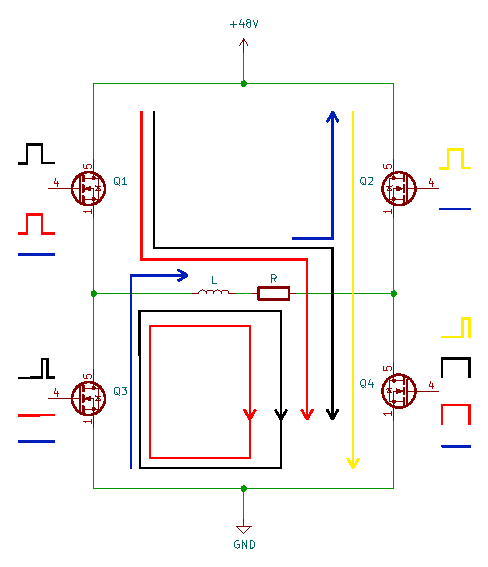
\includegraphics[width=0.7\linewidth]{kapitola4/figures/hbridge_driving.eps}
	\caption{Vše uvažováno pro kladný směr proudu.  Vyznačeného \textbf{černě} pro spínání tranzistorů pro regulační odchylku menší než \SI{5}{\percent} požadovaného proudu,
		\textbf{modře} pro naakumulovanou energii v indukčnosti a vypnuté tranzistory,
		\textbf{žlutě} pro nechtěné současné sepnutí tranzistorů jedné větve}
	\label{fig:mosfet_driving}
\end{figure}


\subsection{Popis a inicializace čítače \texttt{TCC0}}

Pro generování \textit{PWM} signálu pro řízení driverů \textit{MP1917} je čítač \texttt{TCCx} ideální volbou,
neboť některé jeho funkce usnadňují řízení H-můstků.
Funkce \texttt{Non-Recoverable Fault (NRF)} zajišťuje předem definované chování tranzistorů v případě detekce \texttt{NRF},
což je jinými slovy událost \texttt{EVENT\_1} na programátorem definovaném kanálu
(v našem případě nastaveno na kanálu \SI{2}) periferie \texttt{Event\ System}).

Při detekci \texttt{NRF} jsou rozepnuty horní tranzistory  (\textit{Q1} a \textit{Q2} v obr. \ref{fig:mosfet_driving}) a
sepnuty dolní tranzistory \textit{H-můstku} (\textit{Q3} a \textit{Q4} v obr. \ref{fig:mosfet_driving}),
čímž se vytvoří cesta pro vybití energie z indukční zátěže.
Takové chování ilustruje černá smyčka přes tranzistory \textit{Q3} a \textit{Q4} v obr. \ref{fig:mosfet_driving}.


V případě pouhého vypnutí všech tranzistorů si potenciálně naakumolovaná energie v induknčnosti \textit{L}
otevře cestu přes zpětné diody tranzistorů, jak pro kladný směr proudu naznačuje modrá smyčka v obr. \ref{fig:mosfet_driving}
přes zpětné diody tranzistorů \textit{Q2} a \textit{Q3}.
Tímto způsobem se indukčnost \textit{L} sice vybije,
ale hrozí vznik nežádoucího napěťového přepětí ve stejnosměrném meziobvodu.
Proto je jakákoliv deaktivace výstupu realizována generováním \texttt{NRF},
respektive generováním \texttt{Event} na kanálu \SI{2}{},
což zajišťuje bezpečné vybití energie z indukčnosti \textit{L}
a pozastavení čítače \texttt{TCC0} do doby deaktivace \texttt{NRF}.

Další užitečnou funkcí je automatické vkládání \textit{dead-time} mezi spínáním \textit{high-side}
a \textit{low-side} tranzistorů v jedné větvi.
Otevřený tranzistor se totiž zavírá s určitou setrvačností po změně řídícího signálu \textit{gatu} na \SI{0}{\volt},
díky čemuž může dojít ke zkratu napájecího napájení v oné větvi, viz fialově vyznačený proud v obr. \ref{fig:mosfet_driving}).
Vložením vhodně dlouhé doby, kdy se čeká než dojde k sepnutí opačného tranzistoru jedné větve, takzvaný \textit{dead-time},
se předchází zbytečným ztrátám či dokonce destrukci tranzistorů.

Při inicializaci je nejdříve v čítači \texttt{TCC0} povolen hodinový signál a nakonfigurovány piny \texttt{PA20} až \texttt{PA23}.
Registr \texttt{Output Matrix} je nastaven tak,
že \texttt{PA20} a \texttt{PA21} řídí \textit{low-side} tranzistory \textit{Q3} a \textit{Q4},
a \texttt{PA22} a \texttt{PA23} řídí \textit{high-side} tranzistory \textit{Q1} a \textit{Q2} (viz obr. \ref{fig:mosfet_driving}).
Každému výstupnímu pinu odpovídá \texttt{Capture Compare} registr se stejným indexem \texttt{PA2x}:

\begin{table}[htpb]
	\centering
	\caption{Přiřazení CCx registrů k pinům PA20 až PA23}
	\label{table::OTMX_CC_to_PA}
	\begin{tabular}{ll}
		CC0 & PA20 \\
		CC1 & PA21 \\
		CC2 & PA22 \\
		CC3 & PA23 \\
	\end{tabular}
\end{table}

Perioda čítače je nastavena na \SI{2000}{}, což při vstupním kmitočtu \SI{200}{\mega\hertz},
generuje \textit{PWM} s kmitočtem \SI{100}{\kilo\hertz}.
Vložený \textit{dead-time} mezi spínání high a low side tranzistorů jedné větve je \SI{10}{\nano\second},
Je povoleno generování přerušení při přetečení, \texttt{NRF} a jeho registry,
které defunují stavy jednotlivých výstupů při detekci \texttt{NRF}.


\subsection{Řízení H můstku}

Regulační smyčka obsahuje \textit{PID} regulátor,
jehož konstanty byly experimentálně naladěny na základě odezvy systému na obdélníkový požadavek změny proudu a
jeho výsledného průběhu na zátěži. Jako zátěž byla použita indukčnost o velikosti \SI{250}{\micro\henry},
což odpovídá minimální očekáváné hodnotě v budoucnu používaných aktuátorů a akčních členů.
Samotná \textit{DPS} zdroje neobsahuje žádnou filtrační indukčnost,
neboť předpokládané zátěže jsou vždy induktivního charakteru.

\begin{figure}[htpb]
	\centering
	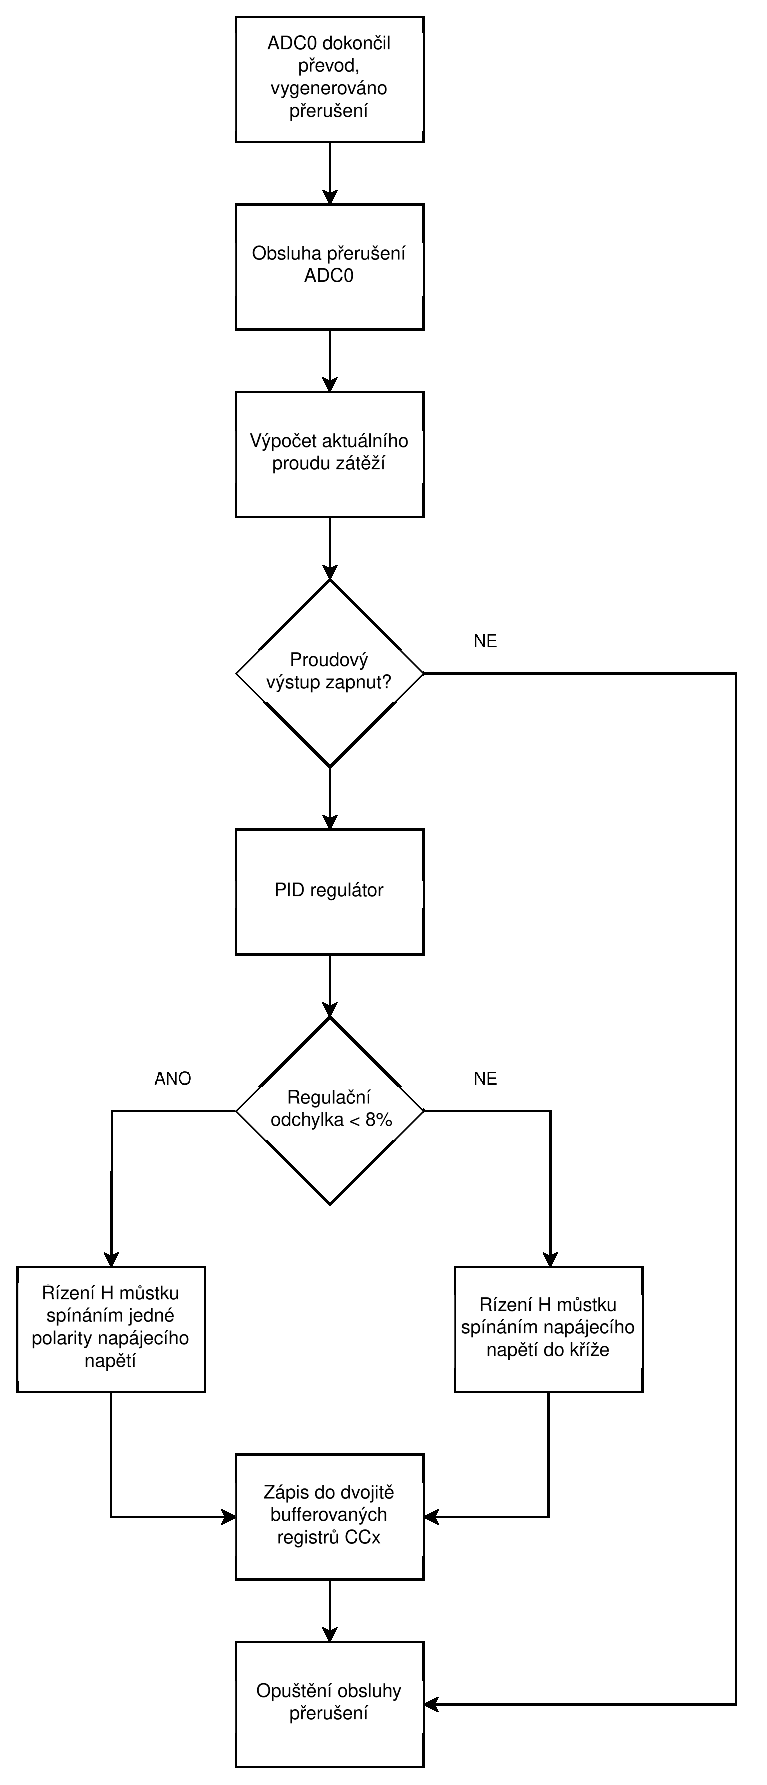
\includegraphics[width=0.6\linewidth]{kapitola4/figures/flowchart_regulator_current.eps}
	\caption{Vývojový diagram proudové regulace}
	\label{fig::flowchart_regulator_curret}
\end{figure}

Vývojový diagram regulace proudu je vidět na obrázku \ref{fig::flowchart_regulator_curret}.
Spuštění regulační smyčky je vázáno na dokončení převodu \texttt{ADC0} a podmíněno povolením proudového výstupu.
Zahájení převodu \texttt{ADC0} je iniciováno přetečením čítače \texttt{TCC0}.
Převodník \texttt{ADC0} je určen výhradně pro měření napětí na proudovém senzoru \textit{INA241B1}.
Po dokončení převodu je vyvoláno přerušení, ve kterém je vypočítána aktuální hodnota proudu na základě změřeného napětí a
převodní konstanty senzoru. Regulační odchylka, definovaná jako rozdíl mezi požadovanou a naměřenou hodnotou proudu,
je následně předána PID regulátoru, který vypočítá nové hodnoty \texttt{CCx} registru čítače \textit{TCC0}.

V kódu je nejdříve vypočítána prahová hodnota regulační odchylky \texttt{error\_th} jako \SI{5}{\percent}
z požadovaného proudu \texttt{current\_request}.
Tato hodnota je následně omezena funkcí \texttt{std::clamp} tak,
aby nebyla menší než \SI{300}{\milli\ampere} a větší než \SI{1000}{\milli\ampere}.
Funkce \texttt{std::clamp} tedy zajišťuje,
že prahová hodnota bude vždy v rozmezí od \SI{300}{\milli\ampere} do \SI{1000}{\milli\ampere},
i když by \SI{5}{\percent} z požadovaného proudu bylo mimo tento rozsah.

Tato prahová hodnota se poté porovnává s aktuální regulační odchylkou \texttt{error\_current}.
Pokud je absolutní hodnota regulační odchylky větší než \texttt{error\_th},
tedy pokud se nachází mimo interval $\langle -\texttt{error\_th}; \texttt{error\_th} \rangle$,
H-můstek řídí proud spínáním tranzistorů do kříže.
Tím je na zátěž přivedena buď kladná, nebo záporná polarita napájecího napětí,
což umožňuje rychlou změnu proudu a velký akční zásah.

Pokud však regulační odchylka zůstává v intervalu $\langle -\texttt{error\_th}; \texttt{error\_th} \rangle$,
strategie řízení se mění:
\begin{itemize}
	\item Trvale je sepnut jeden z \textit{low-side} tranzistorů (podle směru proudu).
	\item Střídavě se spíná \textit{high-side} a \textit{low-side} tranzsitor větve opačné, viz černý průběh na \oref{fig:mosfet_driving}
\end{itemize}

Tento způsob řízení snižuje strmost změn napětí na zátěži,
čímž se snižuje zvlnění proudu a omezuje rušení, zejména u zátěží s malou indukčností.
Zkratování zátěže v opačných cyklech je nezbytné,
aby indukční zátěž mohla k uzavření obvodu využít otevřených tranzistorů namísto jejich zpětných diod,
viz červený průběh na obrázku \ref{fig:mosfet_driving}.
To by způsobovalo zbytečné ztráty,
protože zpětné diody mají větší úbytek napětí než otevřené tranzistory.

Při návrhu byla zohledněna požadovaná rychlost regulační smyčky,
aby bylo možné vypočítat novou hodnotu střídy \textit{PWM} v každé periodě čítače \texttt{TCC0},
což bylo ověřeno experimentálně.
Testování probíhalo tak,
že na začátku regulační smyčky byla aktivována jedna z \textit{LED} a při jejím dokončení byla \textit{LED} opět vypnuta.
Na osciloskopu byl sledován průběh napětí na \textit{LED} a řídicí signály \textit{H-můstku},
přičemž přetečení čítače \texttt{TCC0} bylo na osciloskopu jasně patrné, stejně tak jako i sepnutí a vypnutí signálů LED
Tyto experimenty potvrdily schopnost výpočtu nového regulačního zásahu v každém vzorkovacím okamžiku \texttt{ADC0}.


\subsection{Využití proměnných \texttt{std::atomic}}

Požadovaná hodnota proudu je stanovena uživatelem a uložena
jako amplituda v proměnné \texttt{current\_request}.
Pro stejnosměrný výstup je tato hodnota přímo použita jako referenční proud pro regulaci.
U střídavého výstupu dochází k přenásobování této proměné v metodě přímé digitální syntézy (\textit{DDS}).

V režimu regulace polohy voicecoilu slouží výstup z regulátoru polohy jako požadavek na proud,
tedy opět proměná \texttt{current\_request}, ukládající požadavek na proud.
Proměná je tedy sdílena mezi hlavním programem (zpracování zprávy, viz \nameref{section::mcu_main_run}),
regulátorem proudu (přerušení \texttt{ADC0}), regulátorem polohy (přerušení \texttt{ADC1}, viz \nameref{section::position_regulator})
a \textit{DDS} (přerušení \texttt{TC0}, viz \nameref{section::dds_implementation}).
Výše jmenované úlohy jsou spouštěné nesekvenčně,
všechny zmíněné periferie používají různé kmitočty a
navíc ve všech jmenovaných přerušeních dochází k možnému zápisu do proměné \texttt{current\_request}.
Z tohoto důvodu je pro \texttt{current\_request} použit typ \texttt{std::atomic<float>}.

Standardní proměnné v \textit{C++} nejsou ve výchozím nastavení \textit{thread-safe}, což znamená,
že pokud k nim přistupuje více vláken nebo přerušení současně, může dojít k problémům,
jako je \textit{race condition} nebo \textit{data corruption}.
\texttt{std::atomic} je třída v \textit{C++}, která poskytuje atomické operace.
Atomické operace jsou nedělitelné, což znamená, že se buď provedou celé, nebo vůbec.
Díky tomu je zajištěno, že i když k proměnné přistupuje více vláken nebo přerušení současně,
nedojde k nekonzistenci dat.
Použití atomických proměnných je důležité zejména v těchto situacích:

\begin{itemize}
	\item \textbf{Sdílení dat mezi přerušením a hlavním programem:} Přerušení může zapisovat do proměnné, kterou hlavní program čte. Bez atomických operací by mohlo dojít k tomu, že hlavní program čte nekompletní nebo nekonzistentní data.
	\item \textbf{Sdílení dat mezi více vlákny:} Pokud více vláken přistupuje ke stejné proměnné, atomické operace zajistí, že nedojde k \textit{race condition}.
	\item \textbf{Synchronizace:} Atomické proměnné mohou být použity pro synchronizaci mezi vlákny nebo přerušením a hlavním programem.
\end{itemize}


\section{Regulace polohy}
\label{section::position_regulator}

Pro určení polohy slouží převodník \texttt{ADC1},
který je ihned po startu dedikován k měření teploty jednou za \SI{10}{\second},
viz \nameref{section::System_settings}.
Nicméně v obsluze jeho přerušení bylo dopředu počítano s multiplexem různých vstupů.
Převodník \texttt{ADC1} byl zvolen pro multiplex,
neboť druhý dostupný převodník \texttt{ADC0} využívaný pro měření výstupního proudu je využit na hranici své datové prostupnosti.

Převodník \texttt{ADC1} je nakonfigurován pro měření napětí z Hallovy sondy připojené ke třípinovému konektoru.
Tato sonda poskytuje regulátoru polohy informaci o aktuální poloze jádra lineárního aktuátoru.
Zahájení převodu je řízeno přetečením čítače \texttt{TCC0}, který zároveň generuje \textit{PWM} signál pro řízení \textit{H-můstku}.
Událost přetečení čítače je zpracována pomocí modulu \texttt{Event System},
který umožňuje zahájení převodu bez zásahu hlavního procesoru.
Převodník \texttt{ADC1} reaguje na událost \texttt{EVENT\_0} generovanou čítačem \texttt{TCC0},
pouze pokud je povolena regulace polohy, v opačném případě slouží pouze pro měření teploty.

Po ukončení převodu generuje \texttt{ADC1} přerušení, v jehož obsluze je volán regulační algoritmus pro řízení polohy.
Tento proces se opakuje s periodou přibližně $\approx$~\SI{220}{\micro\second},
která je výrazně delší než samotná perioda přetečení čítače \texttt{TCC0}, a tudíž i generace \textit{PWM}.
Eventy generované čítačem \texttt{TCC0} během aktivního převodu \texttt{ADC1} jsou jednoduše ignorovány.

Výpočet periody převodu AD převodníku je dán vztahem:

\begin{equation}
	T_{\text{ADC}} = \frac{f_{\text{ADC\_CLK}}}{(N_{\text{RES}} + 1) \cdot N_{\text{SAMPLES}}}
	\label{eq:T_ADC1}
\end{equation}

kde:

\begin{itemize}
	\item $f_{\text{ADC\_CLK}}$ – hodinová frekvence převodníku (\SI{15}{\mega\hertz}),
	\item $N_{\text{RES}}$ – bitová hloubka převodu (zde \SI{12}{\bit}),
	\item $N_{\text{SAMPLES}}$ – počet vzorků pro hardwarové průměrování (v tomto případě \num{256}).
\end{itemize}

Dosazením těchto hodnot do rovnice~\eqref{eq:T_ADC1} získáme:

\begin{equation}
	T_{\text{ADC}} = \frac{15 \times 10^{6}}{(12 + 1) \cdot 256} \approx \SI{220}{\micro\second}
	\label{eq:T_ADC1_evaluated}
\end{equation}

Převodník \texttt{ADC1} je navíc periodicky využíván pro měření teploty desky.
Tato měření však probíhají pouze jednou za \SI{10}{\second},
a jejich vliv na vzorkovací frekvenci Hallovy sondy je z praktického hlediska zanedbatelný.


\begin{figure}[htpb]
	\centering
	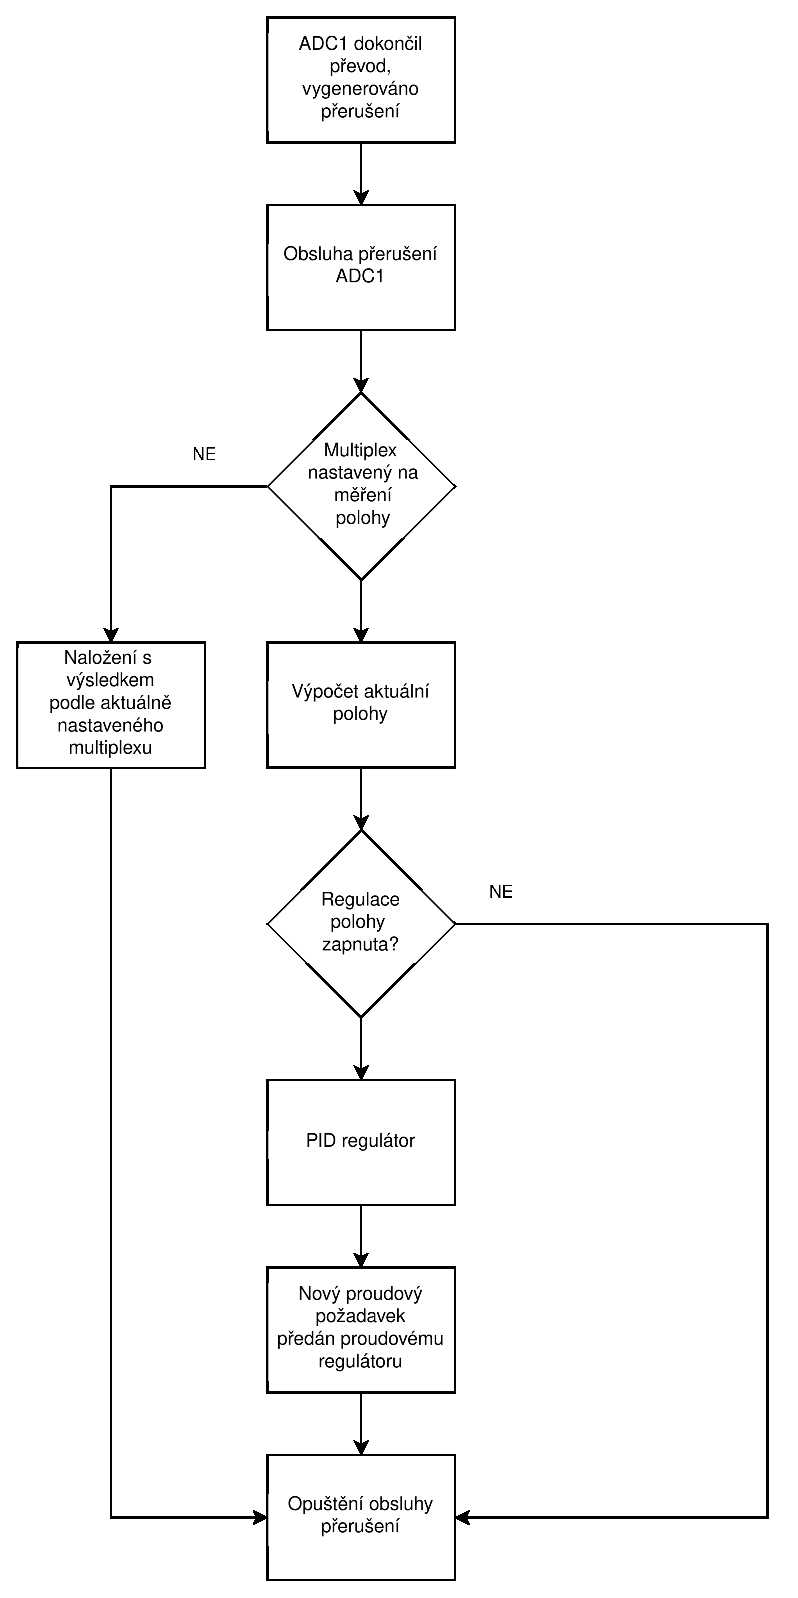
\includegraphics[width=0.6\linewidth]{kapitola4/figures/flowchart_regulator_position.eps}
	\caption{Vývojový diagram regulace polohy}
	\label{fig::flowchart_regulator_position}
\end{figure}

Vývojový diagram regulace polohy je ilustorván na \oref{fig::flowchart_regulator_position}.
Po dokončení převodu je vyvoláno přerušení, ve kterém dochází k výpočtu polohy aktuátoru na základě změřeného napětí.
Převod je realizován pomocí předem zdiskretizované převodní funkce uložené v mikrokontroléru,
viz \nameref{section::hall_perm_magnet}.

Tato převodní funkce byla vytvořena experimentálně.
Nejprve bylo změřeno napětí v závislosti na poloze v několika bodech.
Následně byly naměřené hodnoty interpolovány, zdiskretizovány a uloženy do jednoduchého pole,
kde index odpovídá naměřenému napětí a hodnota v poli reprezentuje odpovídající polohu.
Při samotném převodu se změřené napětí převede na index v tomto poli, jako:

\begin{equation}
	index = \left\lfloor \frac{U_{ADC} - (U_{MIN} + U_{OFFSET})}{(U_{MAX} +  U_{OFFSET}) - (U_{MIN} +  U_{OFFSET})} \cdot ROZSAH \right\rfloor
\end{equation}

kde:
\begin{itemize}
	\item $index$ je index do pole sloužícího jako Look-Up Table,
	\item $U_{ADC}$ je hodnota napětí získaná z ADC převodníku,
	\item $U_{MIN}$ je minimální hodnota napětí v LUT,
	\item $U_{OFFSET}$ je hodnota rozdílu napětí zjištěného v autokalibraci, 
	určujcí rozdíl v napěťové ose mezi funkcí v LUT a skutečnou funkcí,
	\item $U_{MAX}$ je maximální hodnota napětí v LUT,
	\item $ROZSAH$ je velikost pole.
\end{itemize}

Vložením indexu do pole \texttt{h\_interp[index]} dostávám informaci o aktuální poloze.
Regulace polohy je realizována pomocí \textit{PID} regulátoru,
který používá rozdíl požadavku polohy z \textit{DDS} a aktuální polohy z \texttt{h\_interp[index]}.
Parametry \textit{PID} regulátoru byly stanoveny experimentálně na základě odezvy lineárního aktuátoru,
který byl použit v experimentálním vibračním podavači.

Při adresaci \textit{LUT} tabulky pomocí použitého indexu získám aktuální polohu jádra a
získaná hodnota je filtrována exponenciálním klouzavým průměrem pro potlačení příliš rychlých odchylek.
Implementace tohoto filtru odstranila chvění jádra a zlepšila stabilitu polohy.

\begin{lstlisting}[language=C++, caption=Adresace LUT a implementace filtru]
        // Filter parameter (alpha) - Adjust this for smoothing (0.0 < alpha < 1.0)
        static float alpha = 0.33f; // Example: Lower alpha for more smoothing
        static float filtered_position_actual = 0.0f; // Initialize the filter state
        float raw_position_actual = LUT[get_LUT_index()];
        // Apply the EMA filter
        filtered_position_actual = alpha * raw_position_actual + (1.0f - alpha) * filtered_position_actual;
\end{lstlisting}


Výstupem regulátoru polohy je požadovaná hodnota proudu,
která je předána regulátoru proudu implementovanému v metodě \texttt{regulator()} ve třídě \texttt{Current\_source}.

\section{Přímá digitální syntéza}
\label{section::dds}
Pro vytvření střídavých průběhů proudu a pro ovládní polohy linearního aktuátoru bylo použito metod přímé digitální syntézy
(\textit{Direct Digital Synthesis}, \textit{DDS}). 
Tato metoda využívá numerického řízení k vytváření periodických signálů s přesně definovanou frekvencí a fází.

Základem \textit{DDS} je fázový akumulátor a fázový přírůstek:
\begin{itemize}
	\item \textbf{Fázový akumulátor (phase\_accum)}: Jedná se o proměnnou, která uchovává aktuální fázový stav generovaného signálu.
	      S každým vzorkem se jeho hodnota zvyšuje o fázový přírůstek.
	\item \textbf{Fázový přírůstek (phase\_inc)}: Tento parametr určuje krok, o který se fázový akumulátor při každém vzorku posune.
	      Hodnota fázového přírůstku je dána vztahem:
\end{itemize}

\begin{equation}
	f_{OUT} = \frac{\Delta \varphi}{N} \cdot f_{CLK}
	\label{eq::dds}
\end{equation}

kde:
\begin{itemize}
	\item $\Delta \varphi$ je fázový přírůstek,
	\item $f_{OUT}$ je požadovaná výstupní frekvence,
	\item $f_{CLK}$ je hodinová frekvence systému,
	\item $N$ je velikost pole fázového akumulátoru.
\end{itemize}

Maximální frekvence, kterou dokážeme pomoci \textit{DDS} vygenerovat je podle vzorkovacího teorému dána vztahem:
\begin{equation}
	f_{max\_out} = f_{CLK} \cdot \frac{N}{\Delta \varphi_{MAX}} = \frac{f_{CLK}}{2},
	\label{eq::dds_max}
\end{equation}

\subsection{Generování signálu pomocí \textit{DDS}}
Po inkrementaci fázového akumulátoru se jeho hodnota použije jako \texttt{index} pro tabulku vzorků střídavého průběhu \texttt{ac\_lut}.
Tato tabulka obsahuje předpočítané hodnoty chtěné střídavé funkce pro celý rozsah fáze od $0$ do $2\pi$.
Po přetečení hodnoty fázového akumulátoru dochází k restartování jeho hodnoty na 0,
čímž se zajistí periodičnost generovaného signálu.

Výsledný výstupní signál je dán vztahem:

\begin{equation}
	I_{OUT} = Ampl \cdot ac\_lut[phase\_accum] + DC_{OFFSET}
	\label{eq::Iout_DDS}
\end{equation}

kde:
\begin{itemize}
	\item \textbf{Ampl} je uživatelem zadaná amplituda v ampérách, nebo polohový offset v \SI{}{\milli\meter},
	\item \textbf{ac\_lut[phase\_accum]} ukazuje na index pole s uloženou hodnotou odpovídající aktuální fázi,
	\item \textbf{$DC_{OFFSET}$} je stejnosměrný offset přidaný k signálu,
	      může se jednat o proudový offset v ampérách nebo polohový offset v \SI{}{\milli\meter}
\end{itemize}


\subsection{Řešení \textit{DDS} v \textit{MCU}}
\label{section::dds_implementation}

Obsluha syntézy je taktována generováním přerušení při přetečení běžného čítače \textit{TC0}.
Čítač používá jako taktovací hodiny \texttt{GCLK0} s frekvencí \SI{120}{\mega\hertz}
a perioda čítače na \SI{6000}, což generuje přetečení s frekvencí \SI{24}{\kilo\hertz}.
Pole \texttt{ac\_lut} je 2400 floatů veliké.
Pro splnění vzorkovacího teorému, dle \rref{eq::dds_max}, musí platit:

\begin{equation}
	f_{MAX\_OUT} = \frac{f_{CLK}}{2} = \SI{24}{\kilo\hertz},
	\label{eq::dds_max_val}
\end{equation}

V praxi se však obvykle nepoužívá výstupní frekvence blízko $\frac{1}{2}$ taktovací frekvence, 
protože dva vzorky na periodu vedou k velmi špatné rekonsturkci jakéhokoliv signálu.
Vzorky mohou totiž nabývat pouze dvou opačných hodnot, 
což může být například \SI{1}{} a \SI{-1}{}, ale taky \SI{0}{} a \SI{0}{}
a jakéhokoliv kombinace mezi těmito hodnotami.
Navíc vlivem parazitních driftů a posunů kmitočtů dochází k neustálé změně kombinací těchto dvou vzorků.
To vede výstupní signál, který je zatížen parazitní amplitudovou modulací.


A proto se i pro velmi nenáročné aplikace se dá uvažovat maximální užitečná frekvence přibližně jako:

\begin{equation}
	f_{OUT} = f_{MAX\_OUT} = \frac{f_{CLK}}{4},
	\label{eq::dds_real_max_val}
\end{equation}

ovšem pro zajištění ucházejícího harmonického průběhu se doporučuje nejméně 20 vzorků, což znamená:

\begin{equation}
	f_{OUT} = f_{MAX\_OUT} = \frac{f_{CLK}}{20},
\end{equation}


takže po dosazení hodnot implementované \textit{DDS}:

\begin{equation}
	f_{OUT} = f_{MAX\_OUT} = \frac{24000}{4} = \SI{6000}{\hertz},
\end{equation}

respektive:

\begin{equation}
	f_{OUT} = f_{MAX\_OUT} = \frac{24000}{20} = \SI{1200}{\hertz},
\end{equation}

Současná implementace \textit{DDS} umožňuje generování harmonického, trojůhelníkového a obdélníkového signálu,
s libovolným celočíselným fázovým posuvem a stejnosměrným offsetem.
Pro obdélníkový signál lze navíc nastavit střídu a sklon náběžné/doběžné hrany, viz \nameref{section::comunication_protocol}.
Fázový přírůstek je tedy třeba přepočítat při každém zadání frekvence uživatelem.
Z rovnice \eqref{eq::dds_real_max_val} vyplívá maximální frekvence střídavého proudu,
která splňuje požadavek alespoň čtyřech vzorků na jednu periodu signálu, jako \SI{6}{\kilo\hertz}.

Maximální frekvence, kterou může uživatel zvolit je omezena na \SI{2400}{\kilo\hertz},
takže v jedné periodě bude signál tvořen nejméně 10ti vzorky,
ovšem maximální frekvence, kterou zdroj dokáže skutečně vygenerovat je závislá připojené zátěži,
respektive klesá s velikostí indukčnosti zátěže.

\begin{figure}[htpb]
	\centering
	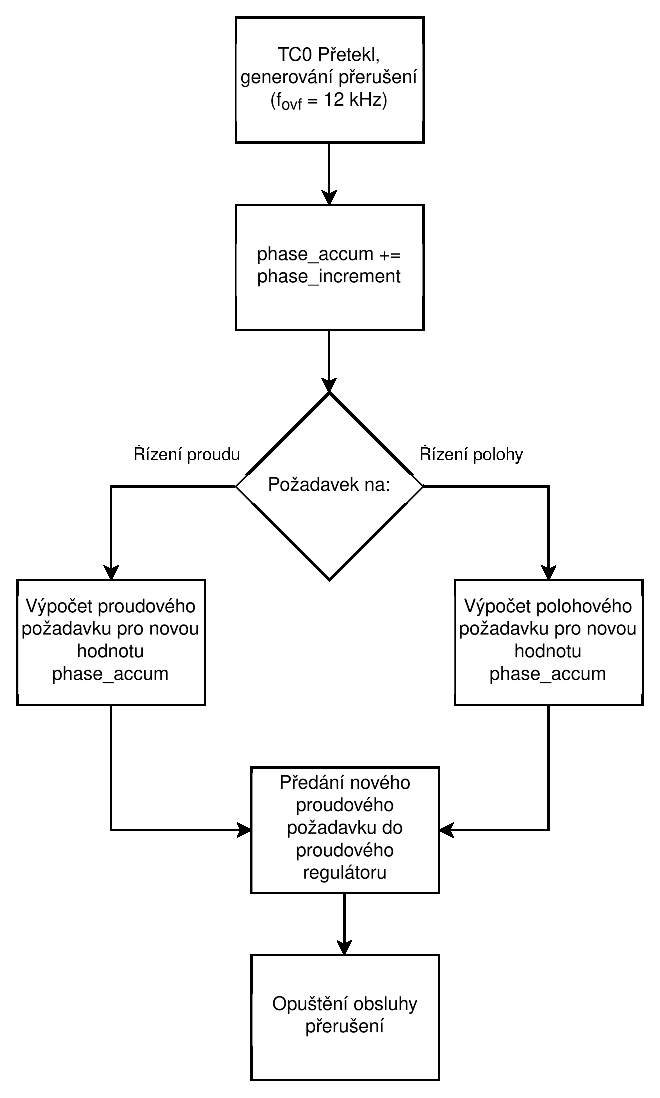
\includegraphics[width=0.5\textwidth]{kapitola4/figures/flowchart_dds.eps} % Cesta k souboru s diagramem
	\caption{Vývojový diagram DDS}
	\label{fig::flowchart_dds}
\end{figure}

V obsluze přerušení dojde k přičtení fázového inkrementu \texttt{phase\_inc} 
k fázovému akumulátoru \texttt{phase\_accum}, viz \ref{fig::flowchart_dds}
a porud vypočítaný dle rovnice \eqref{eq::Iout_DDS}.
Defaultní velikost amplitudy proudu po restartu \texttt{MCU} je \SI{0}{\ampere},
velikost amplitudy polohy \SI{3,5}{\milli\meter}
a OFFSET polohy je \SI{4,5}{\milli\meter}.


\begin{figure}[htpb]
	\centering
	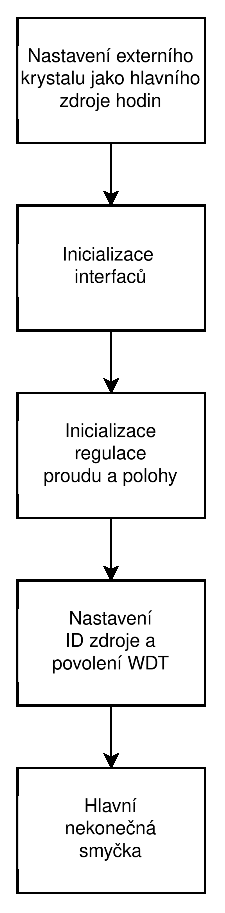
\includegraphics[width=0.15\textwidth]{kapitola4/figures/flowchart_mcu_init.eps} % Cesta k souboru s diagramem
	\caption{Vývojový diagram inicializace}
	\label{fig:mcu_init}
\end{figure}

\section{Běh systému v \texttt{main()}}
\label{section::mcu_main_run}

Po inicializaci systém vstoupí do nekonečné smyčky,
kde se mimo obsluhu přerušení periodicky provádějí následující úkoly:

\begin{enumerate}
	\item Obsluha zdroje proudu pomocí \texttt{aron::Current\_source::handler()}.
	      Tato funkce kontroluje, zda byl odeslán požadavek na vypnutí zdroje.
	      Pokud ano, provede se vypnutí.
	\item Obsluha příjmu zpráv po \textit{UARTu} a \textit{CANu} pomocí \texttt{aron::Communication::rx\_handler()}.
	      Ta zpracovává data přijatá po \textit{UARTu} . Kontroluje FIFO buffer, zda přišla data.
	      Samotný FIFO buffer se plní v přerušení.
	      Také kontroluje, zda přišla nová zpráva po \textit{CAN} sběrnici.
	      Zprávy z \textit{CANu} se do interního bufferu řadiče \texttt{CAN1} ukládají bez činnosti procesoru.
	      Pokud přišla zpráva po kterémkoliv rozhraní, pak ji odešle ke zpracování.
	\item Periodická aktualizace stavových \textit{LED} diod (každých 500 ms).
	\item Periodické spouštění měření teploty (každých 10 s).
	\item Kontrola stisknutí tlačítka. Krátký stisk tlačítka přepíná stav zdroje proudu (zapnuto/vypnuto).
	      Dlouhé podržení tlačítka (déle než 3 sekundy) způsobí restart mikrokontroléru.
	\item Pravidelné krmení Watchdog timeru pomocí funkce \texttt{watch\_dog\_reset()}.
	      Ten se resetuje zápisem hodnoty 0x5A do jeho \texttt{CC} registru.
\end{enumerate}

\begin{figure}[htbp]
	\centering
	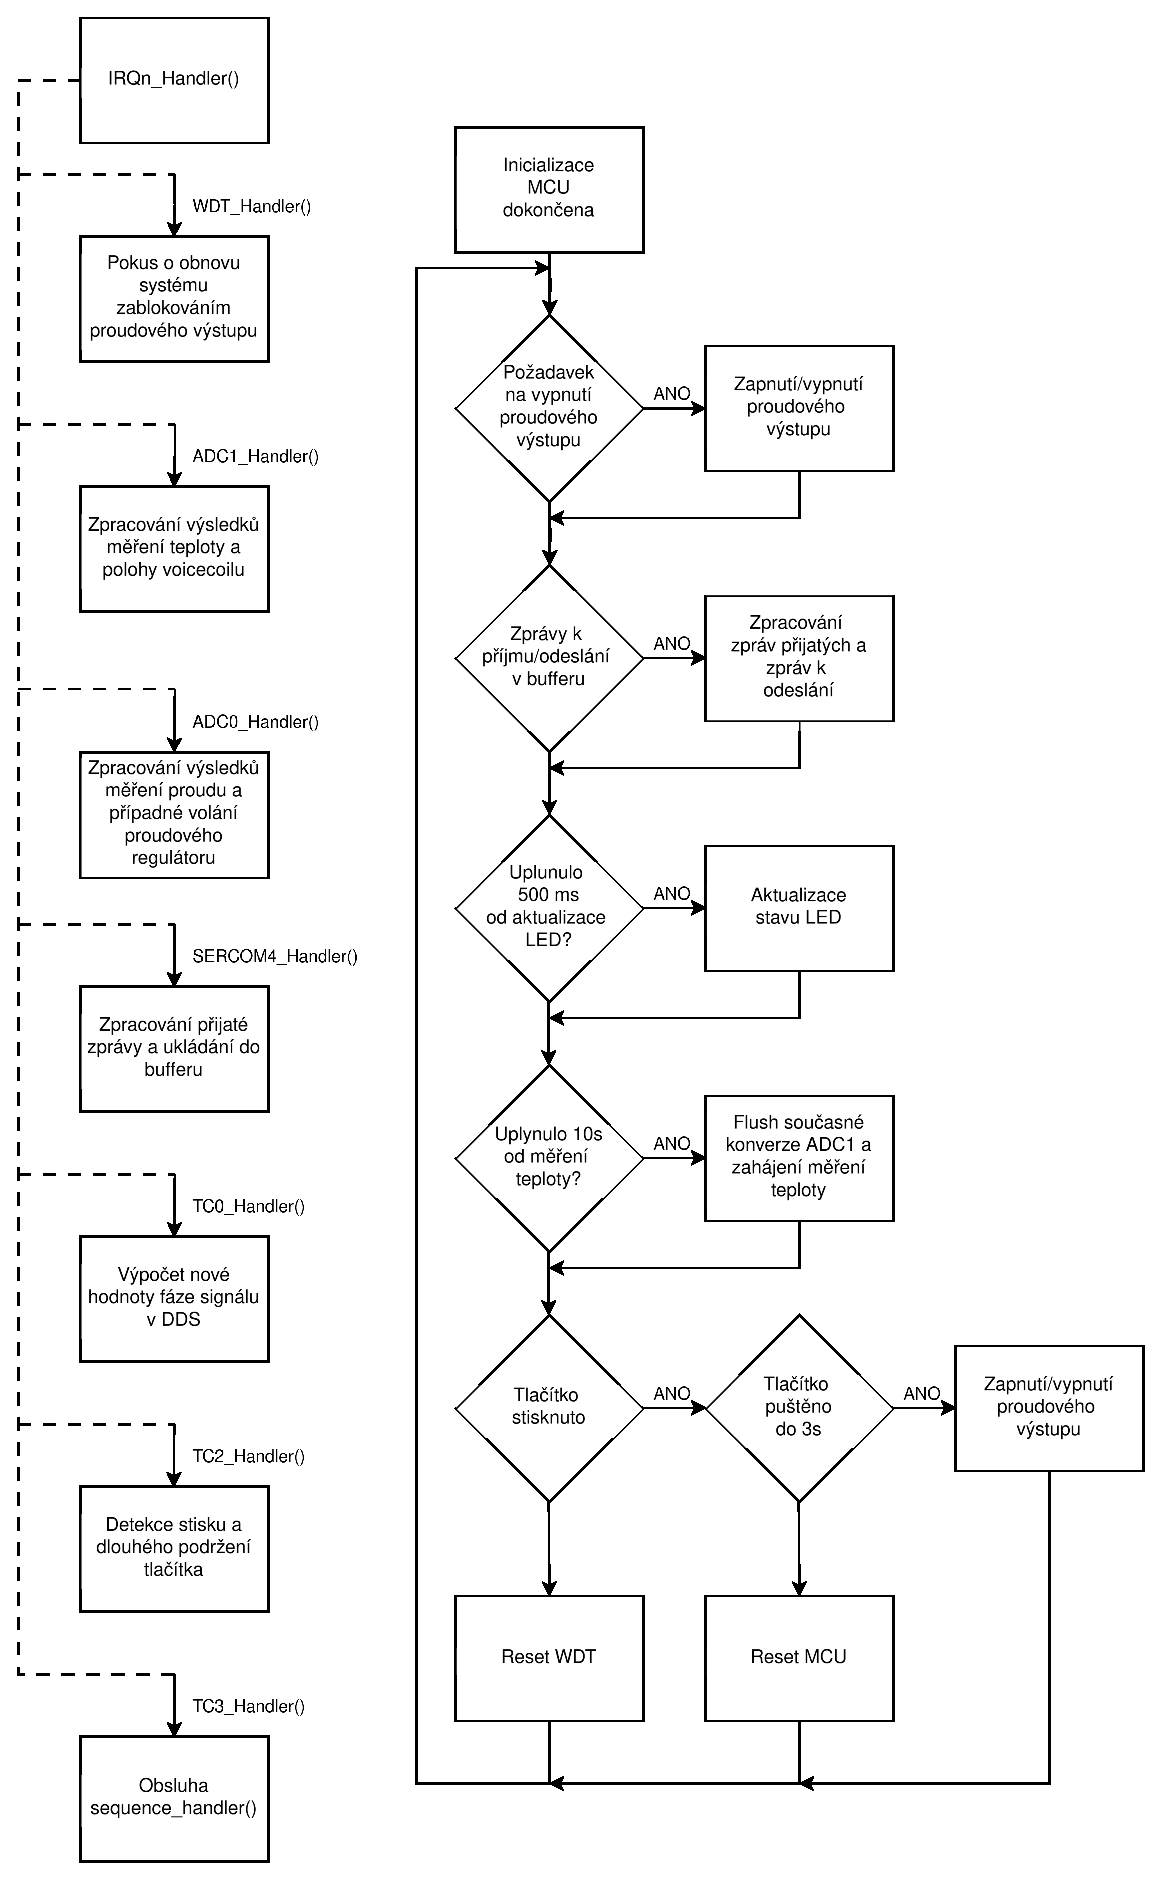
\includegraphics[width=0.9\textwidth]{kapitola4/figures/flowchart_mcu_run.eps} % Cesta k souboru s diagramem
	\caption{Vývojový diagram běhu systému}
	\label{fig:mcu_run}
\end{figure}


\subsection{Popis přerušení}

Systém využívá několik přerušení pro obsluhu různých událostí:

\begin{itemize}
	\item \texttt{WDT\_Handler()}: Obsluha přerušení Watchdog timeru. Vypne výstup v případě, že WDT zahlásí varování.
	      Je to poslední pokus o záchranu běhu systému bez tvrdého restartu.
	\item \texttt{ADC1\_Handler()}: Obsluha přerušení od \texttt{ADC1}.
	      Zpracovává výsledky měření teploty a polohy voicecoilu. Pokud je teplota překročena, zavolá zablokování výstupu.
	      V případě povolené regulace polohy volá regulaci polohy.
	\item \texttt{ADC0\_Handler()}: Obsluha přerušení od \texttt{ADC0}.
	      Zpracovává výsledky měření proudu a případné volání proudového regulátoru
	\item \texttt{SERCOM4\_Handler()}: Obsluha přerušení \texttt{UARTu}.
	      Zpracovává přijaté zprávy a ukládá do bufferu.
	\item \texttt{TC0\_Handler()}: Obsluha přerušení časovače \texttt{TC0}. Používá se pro generování \textit{DDS} signálu.
	\item \texttt{TC2\_Handler()}: Obsluha přerušení časovače \texttt{TC2}. Detekce stisku a dlouhého podržení tlačítka.
	\item \texttt{TC3\_Handler()}: Obsluha přerušení časovače \texttt{TC3}. Obsluha \texttt{sequence\_handler()}.
\end{itemize}
\newpage

\chapter{Měření charakteristik zdroje}

Tato kapitola se zaměřuje na experimentální ověření klíčových charakteristik navrženého proudového zdroje.
Podrobně popisuje provedená měření stejnosměrného i střídavého proudového výstupu, dynamické odezvy na změny zátěže, účinnosti a ztrát,
teplotního zatížení a úrovně generovaného šumu a rušení. Cílem těchto měření bylo kvantifikovat výkonové parametry zdroje,
posoudit jeho stabilitu a kvalitu výstupního signálu v různých provozních podmínkách.
Výsledky těchto analýz poskytují komplexní pohled na funkční vlastnosti a limity navrženého zařízení.

\section{Stejnosměrný proudový výstup}


Ve stejnosměrném režimu byly provedeny měření výstupního proudu, jeho efektivní hodnoty a zvlnění.
Cílem bylo zhodnotit stabilitu výstupu při různých vstupních napětích a zátěžových podmínkách
a jeho výsledky jsou uvedeny v tabulce \ref{tab:dc_measurements}.

\begin{table}[htbp]
	\centering
	\caption{Výsledky měření výstupního proudu, zvlnění a efektivní hodnoty}
	\setlength{\tabcolsep}{4pt}
	\renewcommand{\arraystretch}{1.2}

	\begin{tabular}{|c|*{8}{c|}}
		\hline
		\multicolumn{9}{|c|}{$U_{\text{vstupní}} = \SI{12}{\volt}$ pro \SI{1}{\ohm} \text{zátěž s indukčností }\SI{720}{\micro\henry}} \\
		\hline
		$I_{\text{nastavený}}$ (\si{\ampere}) & -8,00 & -4,00 & -1,00 & -0,10 & 0,10  & 1,00 & 4,00  & 8,00                            \\
		\hline
		$I_{\text{výstup}}$ (\si{\ampere})    & -8,32 & -4,16 & -1,02 & -0,10 & 0,15  & 0,99 & 4,07  & 8,21                            \\
		\hline
		$I_{\text{zvlnění}}$ (\si{\ampere})   & 0,03  & 0,02  & 0,01  & 0,01  & 0,02  & 0,01 & 0,02  & 0,03                            \\
		\hline
		Zvlnění (\%)                          & 0,35  & 0,55  & 1,38  & 10,58 & 11,69 & 1,42 & 0,54  & 0,32                            \\
		\hline
		$I_{\text{RMS}}$ (\si{\ampere})       & 8,32  & 4,16  & 1,02  & 0,10  & 0,16  & 0,99 & 4,07  & 8,21                            \\
		\hline

		\multicolumn{9}{|c|}{$U_{\text{vstupní}} = \SI{48}{\volt}$ pro \SI{1}{\ohm} \text{zátěž s indukčností }\SI{720}{\micro\henry}} \\
		\hline
		$I_{\text{nastavený}}$ (\si{\ampere}) & -8,00 & -4,00 & -1,00 & -0,10 & 0,10  & 1,00 & 4,00  & 8,00                            \\
		\hline
		$I_{\text{výstup}}$ (\si{\ampere})    & -8,36 & -4,36 & -1,06 & -0,24 & 0,14  & 1,04 & 4,35  & 8,42                            \\
		\hline
		$I_{\text{zvlnění}}$ (\si{\ampere})   & 1,29  & 0,47  & 0,10  & 0,05  & 0,02  & 0,08 & 0,44  & 1,35                            \\
		\hline
		Zvlnění (\%)                          & 15,42 & 10,77 & 9,26  & 18,44 & 17,14 & 7,98 & 10,18 & 16,03                           \\
		\hline
		$I_{\text{RMS}}$ (\si{\ampere})       & 8,46  & 4,39  & 1,06  & 0,25  & 0,14  & 1,04 & 4,38  & 8,53                            \\
		\hline

		\multicolumn{9}{|c|}{$U_{\text{vstupní}} = \SI{48}{\volt}$ pro \SI{3}{\ohm} \text{zátěž s indukčností }\SI{720}{\micro\henry}} \\
		\hline
		$I_{\text{nastavený}}$ (\si{\ampere}) & -8,00 & -4,00 & -1,00 & -0,10 & 0,10  & 1,00 & 4,00  & 8,00                            \\
		\hline
		$I_{\text{výstup}}$ (\si{\ampere})    & -8,20 & -4,16 & -1,08 & -0,24 & 0,11  & 0,91 & 4,00  & 7,90                            \\
		\hline
		$I_{\text{zvlnění}}$ (\si{\ampere})   & 0,68  & 0,24  & 0,04  & 0,04  & 0,03  & 0,05 & 0,29  & 0,62                            \\
		\hline
		Zvlnění (\%)                          & 8,27  & 5,66  & 3,87  & 15,68 & 23,42 & 5,71 & 7,17  & 7,85                            \\
		\hline
		$I_{\text{RMS}}$ (\si{\ampere})       & 8,23  & 4,16  & 1,08  & 0,24  & 0,11  & 0,91 & 4,01  & 7,92                            \\
		\hline
	\end{tabular}
	\label{tab:dc_measurements}
\end{table}

Graf \ref{fig::zavislost_proudu} ukazuje závislost výstupního proudu na nastaveném proudu pro různá vstupní napětí.
Zatěžovací charakteristika zdroje je znázorněna v grafu \ref{fig::zatezovaci_char}
a relativní zvlnění výstupního proudu je zobrazeno v grafu \ref{fig::dc_zvlneni}.
Měření ukazují, že výstupní proud dobře kopíruje nastavenou hodnotu s minimální odchylkou.
Největší relativní zvlnění se projevilo při malých proudech, což je běžné u spínaných napájecích zdrojů,
kde je dominantní šum a nelinearity regulace.



\begin{figure}[htpb]
	\centering
	\includegraphics[width=0.95\textwidth]{kapitola5/Figures/Graf1_Vystupni_charakteristika.png} % Cesta k souboru s diagramem
	\caption{Velikost výstupního proudu v závislosti na nastaveném proudu}
	\label{fig::zavislost_proudu}
\end{figure}


\begin{figure}[htpb]
	\centering
	\includegraphics[width=0.95\textwidth]{kapitola5/Figures/Graf2_Zatezova_char_proud.png} % Cesta k souboru s diagramem
	\caption{Zatěžovací charakteristika zdroje}
	\label{fig::zatezovaci_char}
\end{figure}


\begin{figure}[htpb]
	\centering
	\includegraphics[width=0.95\textwidth]{kapitola5/Figures/Graf3_Zvlneni_proudu.png} % Cesta k souboru s diagramem
	\caption{Relativní zvlnění výstupního proudu v závislosti na nastaveném proudu a vstupním napětí}
	\label{fig::dc_zvlneni}
\end{figure}

\section{Střídavý proud}


Pro určení kvalitativních vlastností výstupního střídavého proudu byla změřena efektivní hodnota výstupního proudu
a spektrum výstupního signálu pro různé tvary signálu, nastavené proudy a vstupní napětí.
Na základě těchto měření bylo určeno celkové harmonické zkreslení (THD) výstupního proudu,
které je znázorněno v grafu \ref{fig::ac_THD}.

Celkové harmonické zkreslení (THD) slouží jako ukazatel kvality výstupního střídavého proudu.
Pro ideální sinusový signál by THD mělo být co nejnižší (blízko \SI{0}{\percent}).
Naproti tomu ideální obdélníkový a trojúhelníkový průběh vykazují přirozeně vyšší THD hodnoty,
asice \SI{48.3}{\percent} a \SI{12,1}{\percent}.

\begin{table}[htbp]
	\centering
	\caption{Výsledky měření výstupního střídavého proudu, základní harmonické a harmonického zkreslení pro různé tvary signálu}
	\setlength{\tabcolsep}{4pt}
	\renewcommand{\arraystretch}{1.2}
	\begin{tabular}{|c|*{9}{c|}}
		\hline
		                                  & \multicolumn{3}{c|}{\textbf{Harmonický 10 Hz}} & \multicolumn{3}{c|}{\textbf{Obdélníkový 10 Hz}} & \multicolumn{3}{c|}{\textbf{Trojúhelníkový 10 Hz}}                                                 \\
		\hline
		$I_{\text{nast.}}$ (\si{\ampere}) & 1,00                                           & 4,00                                            & 8,00                                               & 1,00  & 4,00  & 8,00  & 1,00  & 4,00  & 8,00  \\
		\hline

		\multicolumn{10}{|c|}{$U_{\text{vstupní}} = \SI{12}{\volt}$}                                                                                                                                                                              \\
		\hline
		$I_{\text{ef}}$ (\si{\ampere})    & 0,75                                           & 2,94                                            & 5,80                                               & 1,03  & 4,06  & 8,11  & 0,60  & 2,37  & 4,72  \\
		\hline
		$I_1$ (\si{\deci\bel})            & -2,52                                          & 9,26                                            & 15,08                                              & -0,61 & 11,29 & 17,29 & -4,63 & 7,43  & 13,41 \\
		\hline
		$I_1$ (\si{\ampere})              & 0,75                                           & 2,90                                            & 5,67                                               & 0,93  & 3,67  & 7,32  & 0,59  & 2,35  & 4,68  \\
		\hline
		THD (\%)                          & 10,28                                          & 15,67                                           & 21,14                                              & 47,49 & 47,65 & 47,69 & 18,68 & 11,51 & 12,64 \\
		\hline

		\multicolumn{10}{|c|}{$U_{\text{vstupní}} = \SI{48}{\volt}$}                                                                                                                                                                              \\
		\hline
		$I_{\text{ef}}$ (\si{\ampere})    & 0,77                                           & 3,04                                            & 5,78                                               & 1,07  & 4,16  & 8,07  & 0,63  & 2,47  & 4,80  \\
		\hline
		$I_1$ (\si{\deci\bel})            & -2,53                                          & 9,31                                            & 14,78                                              & -0,52 & 11,26 & 17,01 & -4,13 & 7,75  & 13,51 \\
		\hline
		$I_1$ (\si{\ampere})              & 0,75                                           & 2,92                                            & 5,48                                               & 0,94  & 3,65  & 7,09  & 0,62  & 2,44  & 4,74  \\
		\hline
		THD (\%)                          & 21,86                                          & 28,95                                           & 33,37                                              & 54,33 & 54,43 & 54,44 & 20,06 & 15,56 & 16,37 \\
		\hline
	\end{tabular}
	\label{tab:ac_measurements}
\end{table}


\begin{figure}[htpb]
	\centering
	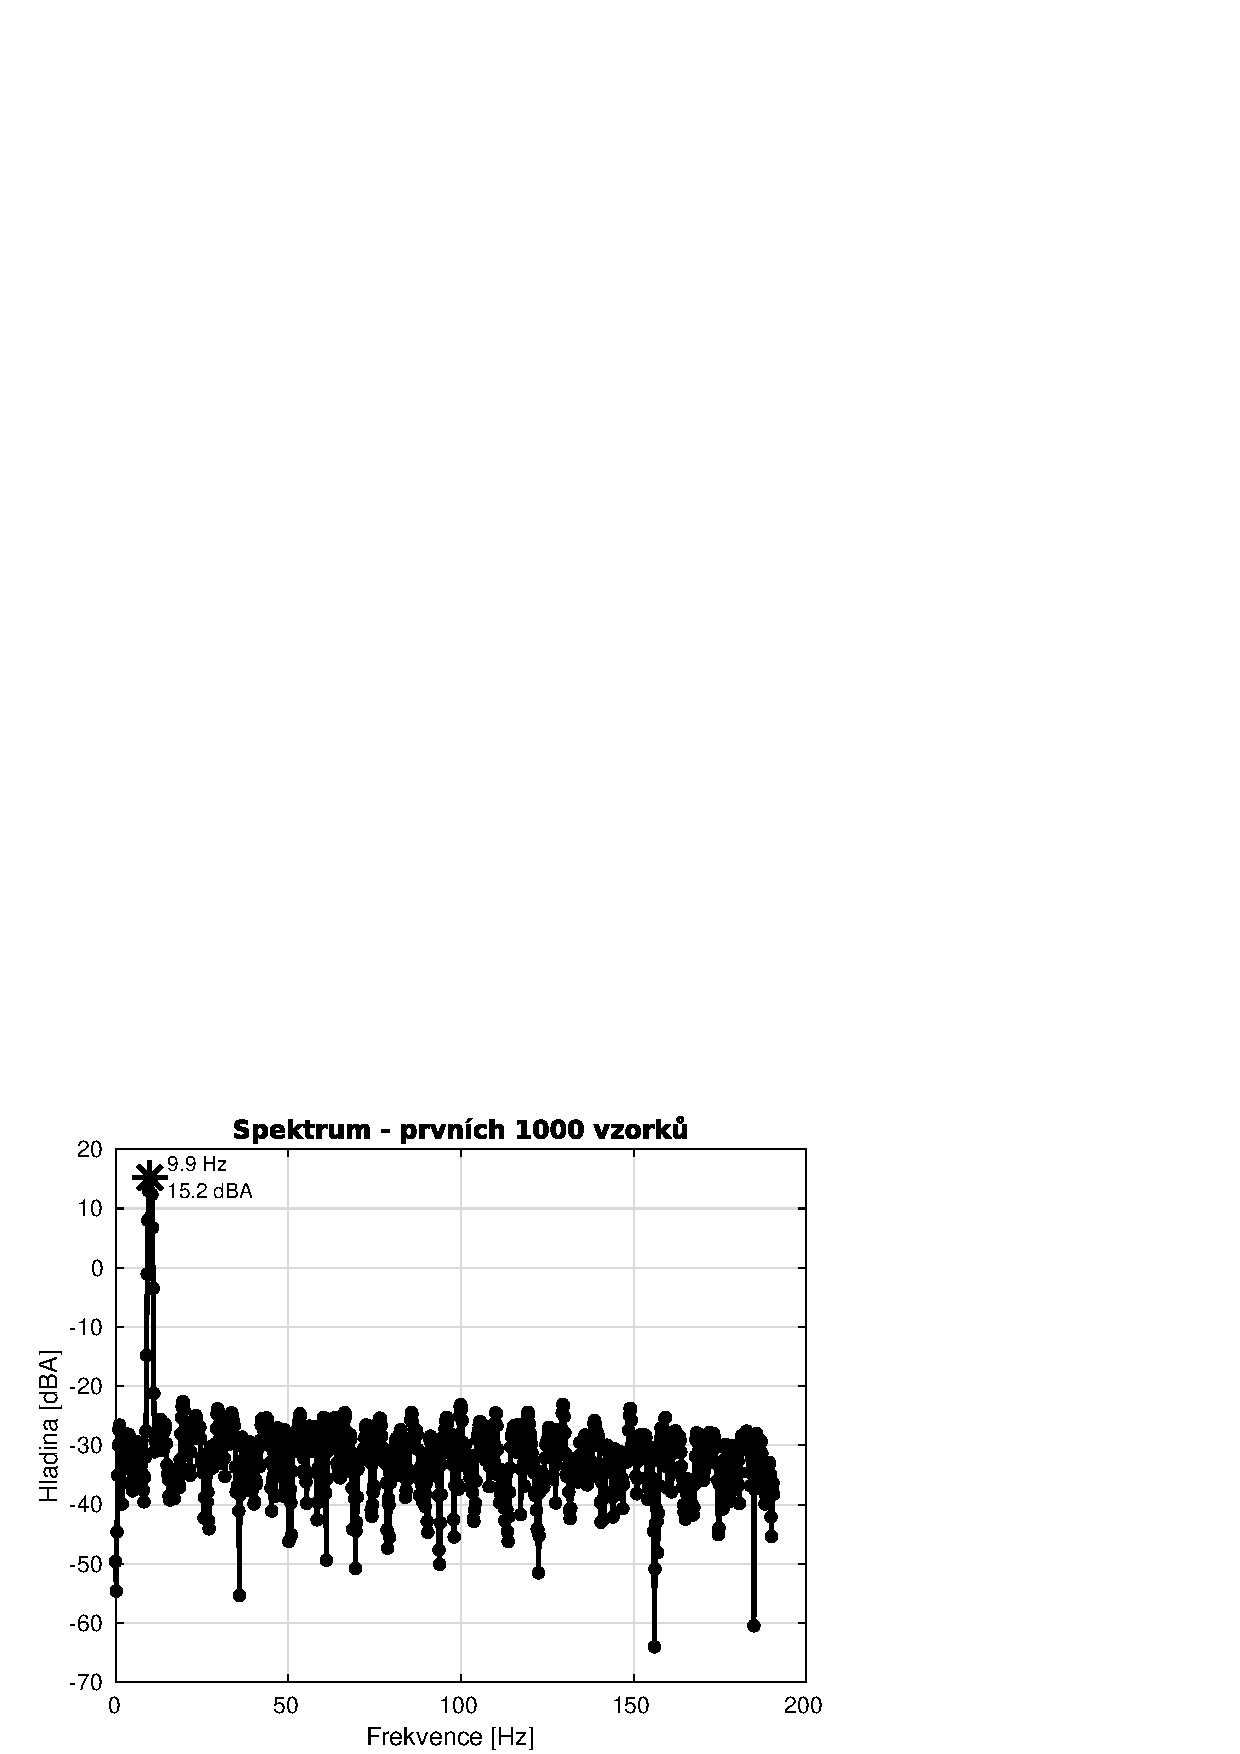
\includegraphics[width=0.95\textwidth]{kapitola5/Figures/sin10hz_8amp_12V.png}
	\caption{Část spektra výstupního proudu do \SI{200}{Hz} pro sinusový průběh \SI{10}{Hz} při \SI{8}{A} a \SI{12}{V}}
	\label{fig::spectrum_sin10hz}
\end{figure}

\begin{figure}[htpb]
	\centering
	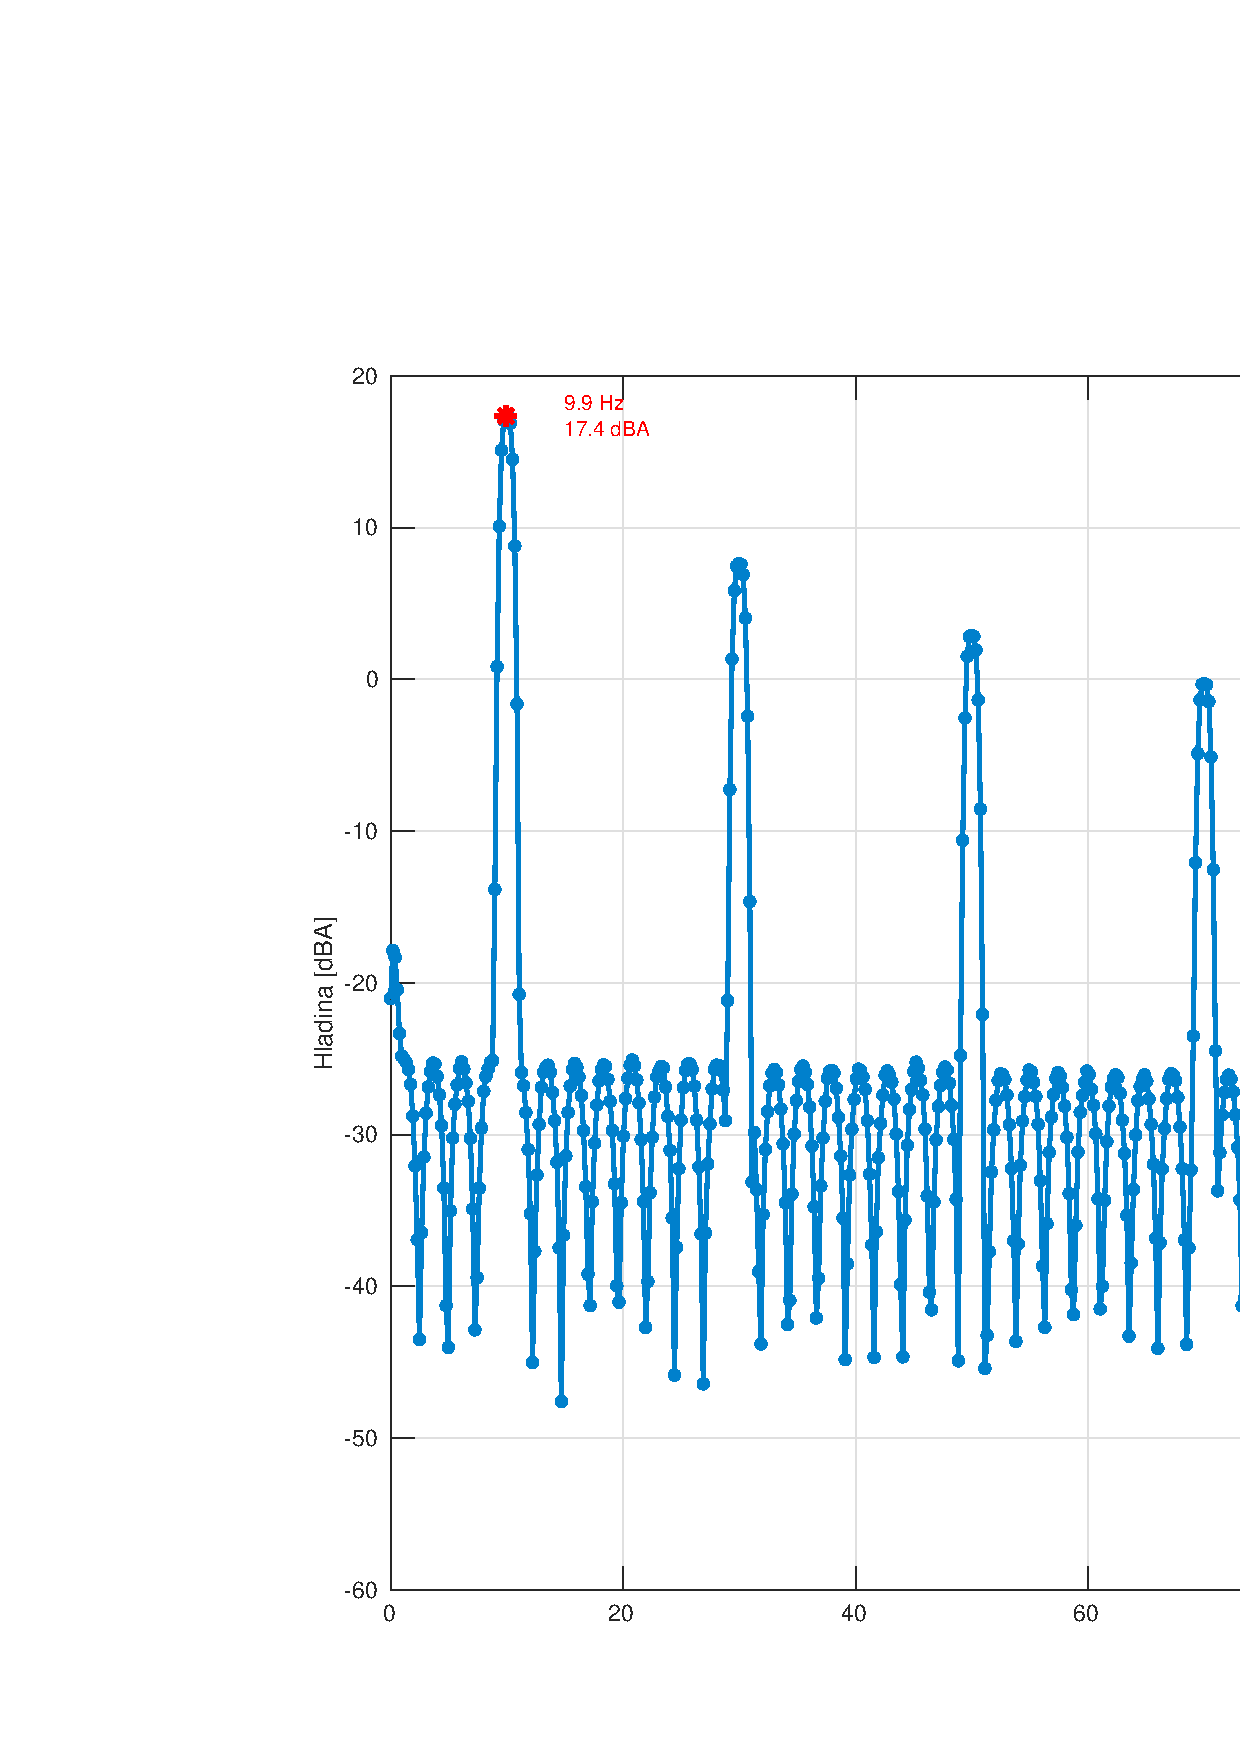
\includegraphics[width=0.95\textwidth]{kapitola5/Figures/SQ10HZ_8A_12V.png}
	\caption{Část spektra výstupního proudu do \SI{200}{Hz} pro obdélníkový průběh \SI{10}{Hz} při \SI{8}{A} a \SI{12}{V}}
	\label{fig::spectrum_SQ10HZ}
\end{figure}

\begin{figure}[htpb]
	\centering
	\includegraphics[width=0.95\textwidth]{kapitola5/Figures/nastavena_realna_amplituda.png} % Cesta k souboru s diagramem
	\caption{Změřená závislost nastaveného a reálné amplitudy}
	\label{fig::ac_first_harmonic}
\end{figure}

\begin{figure}[htpb]
	\centering
	\includegraphics[width=0.95\textwidth]{kapitola5/Figures/THD_AC.png} % Cesta k souboru s diagramem
	\caption{Vypočítané celkové harmonické zkreslení (THD) pro různé tvary signálu}
	\label{fig::ac_THD}
\end{figure}

Výsledky potvrzují očekávaný trend – sinusový průběh má nejnižší zkreslení,
zatímco obdélníkový vykazuje nejvyšší hodnoty THD.
Zjištěné hodnoty THD jsou dostačujicí pro potřeby napájení elektromagnetických aktuátorů.

\section{Dynamická odezva}

Pro posouzení dynamické odezvy zdroje na rychlé změny zátěže byly provedeny skokové změny odporu,
viz \oref{fig::dynamic_load_hlower} a \oref{fig::dynamic_load_higher}.
Reakce byla snímána pomocí osciloskopu při konstantním nastavení proudu \SI{3}{\ampere}.
Výsledky demonstrují schopnost regulátoru rychle stabilizovat výstup.
Tato zátěž (resp. proud) byla zvolena, protože představuje maximální proud,
který je zdroj schopen dodat při vstupním napětí \SI{12}{\volt}, aniž by byl výstupní proud omezen pouze odporem zátěže.
Vstupní napětí \SI{12}{\volt} bylo zvoleno proto,
že při tomto napětí je výstupní proud nejméně ovlivněn rušením a skoková změna zátěže je na osciloskopu nejlépe pozorovatelná.
Zdroj vykazuje rychlou a stabilní reakci s minimálním přechodovým zvlněním.

\begin{figure}[htpb]
	\centering
	\includegraphics[width=0.95\textwidth]{kapitola5/Figures/DUPRR_12V_3A.png} % Cesta k souboru s diagramem
	\caption{Reakce na skokové zvýšení odporu zátěže z $\SI{0.4}{\ohm}$ na $\SI{3.4}{\ohm}$ při konstantním nastaveném proudu $\SI{3}{\ampere}$}
	\label{fig::dynamic_load_higher}
\end{figure}

\begin{figure}[htpb]
	\centering
	\includegraphics[width=0.95\textwidth]{kapitola5/Figures/DYNLOWER_12V.png} % Cesta k souboru s diagramem
	\caption{Reakce na skokové snížení odporu zátěže z $\SI{3.4}{\ohm}$ na $\SI{0.4}{\ohm}$ při konstantním nastaveném proudu $\SI{3}{\ampere}$}
	\label{fig::dynamic_load_hlower}
\end{figure}


\section{Účinnost a ztráty}

Účinnost byla určena jako poměr výstupního a vstupního výkonu.
Při zatížení \SI{8}{\ampere} a napětí \SI{31}{\volt} dosahuje zdroj maximální účinnosti \SI{91.66}{\percent}.
Nižší účinnost při malých výkonech je způsobena relativně vyššími ztrátami v řídicích a spínacích obvodech,
které se v tomto režimu stávají dominantními.
Vstupní výkon byl měřen pomocí laboratorního zdroje s integrovaným měřením dodávaného výkonu.
Výstupní zdánlivý výkon byl odvozen z efektivní hodnoty napětí a proudu pomocí dvou multimetrů.
Zátěž se známou indukčností a odporem umožnila výpočet činného výkonu dodávaného do zátěže (tabulka \ref{tab:efficiency_dc}).

\begin{table}[htbp]
    \centering
    \caption{Výsledky měření účinnosti ve stejnosměrném režimu}
    \setlength{\tabcolsep}{10pt}
    \renewcommand{\arraystretch}{1.2}
    
    \begin{tabular}{|c|*{3}{c|}}
        \hline
        \multicolumn{4}{|c|}{\textbf{Stejnosměrný režim (DC)}} \\
        \hline
        \multicolumn{4}{|c|}{$U_{\text{vstupní}} = \SI{12}{\volt}$ pro zátěž $R = \SI{1,2}{\ohm}$ o indukčnosti $\SI{720}{\micro\henry}$} \\
        \hline
        Nastavený proud $I_{\text{nast.}}$ (\si{\ampere}) & 1,00 & 4,00 & 8,00 \\
        \hline
        Výstupní proud $I_{\text{výst.}}$ (\si{\ampere}) & 0,90 & 3,93 & 8,06 \\
        \hline
        Výstupní výkon $P_{\text{výst.}}$ (\si{\watt}) & 0,97 & 18,49 & 77,96 \\
        \hline
        Vstupní výkon $P_{\text{vst.}}$ (\si{\watt}) & 1,99 & 22,28 & 88,80 \\
        \hline
        Účinnost $\eta$ (\%) & 48,57 & 82,97 & 87,79 \\
        \hline
        
        \multicolumn{4}{|c|}{$U_{\text{vstupní}} = \SI{31}{\volt}$ pro zátěž $R = \SI{1,2}{\ohm}$ o indukčnosti $\SI{720}{\micro\henry}$} \\
        \hline
        Nastavený proud $I_{\text{nast.}}$ (\si{\ampere}) & 1,00 & 4,00 & 8,00 \\
        \hline
        Výstupní proud $I_{\text{výst.}}$ (\si{\ampere}) & 0,90 & 4,30 & 8,36 \\
        \hline
        Výstupní výkon $P_{\text{výst.}}$ (\si{\watt}) & 0,96 & 22,19 & 83,87 \\
        \hline
        Vstupní výkon $P_{\text{vst.}}$ (\si{\watt}) & 2,33 & 27,00 & 91,50 \\
        \hline
        Účinnost $\eta$ (\%) & 41,29 & 82,18 & 91,66 \\
        \hline
    \end{tabular}
    \label{tab:efficiency_dc}
\end{table}

\begin{figure}[htpb]
	\centering
	\includegraphics[width=0.95\textwidth]{kapitola5/Figures/Analyza_ucinnosti_DC.png} % Cesta k souboru s diagramem
	\caption{Změřená účinnost zdroje ve stejnosměrném režimu}
	\label{fig::ac_efficiency}
\end{figure}


\section{Teplotní zatížení}

Po hodině provozu při výstupním proudu \SI{8}{\ampere} a
napájecím napětí \SI{48}{\volt} dosáhla teplota na povrchu výkonových tranzistorů hodnoty \SI{92,4}{\degreeCelsius},
což je s rezervou v mezích doporučených výrobcem, viz \cite{ISC080N10NM6_ds}.

\section{Šum a rušení}

Měření v EMC komoře ukázala,
že bez dodatečných filtračních obvodů zdroj nesplňuje požadavky norem na elektromagnetickou kompatibilitu,
viz (viz přílohy \ref{priloha:mereni_emc_standby} a \ref{priloha:mereni_emc_on}).
Nejproblematičtější jsou přechodové jevy při spínání výkonových tranzistorů,
které generují výrazné vysokofrekvenční složky.
Návrh vhodného LC filtru na vstupu a výstupu spolu s použitím snubberů může tyto projevy významně omezit.
Na základě měření v EMC komoře je však možné určit vhodné parametry pro návrh filtru.

\newpage

\chapter{Vibrační podavač s voicecoily firmy \emph{DESSEQ}}
\label{sec::voicecoil_function}

Běžné vibrační podavače generují vibrace pomocí rotačních vibrátorů,
což jsou elektrické motory, na jejichž hřídeli je umístěno nevyvážené závaží.
Při otáčení motoru vznikají oscilace v důsledku tohoto nevyvážení rotačního ústrojí.
U takového typu vibrátoru lze řídit pouze výkon otáčky, což má přímý vliv na frekvenci oscilací.

Motivací pro použití vibračního podavače na principu voicecoilu je možnost širšího řízení,
které zahrnuje nejen frekvenci oscilací, ale i jejich amplitudu, výšku vysunutí jádra voicecoilu a
fázi oscilací mezi jednotlivými voicecoily.
Tento přístup umožňuje mnohem přesnější kontrolu nad rychlostí a směrem pohybu součástek po platě,
zejména při kombinaci s dodatečnou snímaním a vyhodnocováním polohy součástek pomocí obrazu z kamery.
Tímto způsobem lze dosáhnout vyšší přesnosti a efektivity při manipulaci jak s drobnými, tak s velkými součástkami.


\begin{figure}[htbp]
	\centering
	\includegraphics[width=0.95\textwidth]{kapitola6/Figures/vibration_desk.png}
	\caption{Testend vibrační stolice firmy \emph{DESSEQ}}
	\label{fig::vibrator_DESSEQ}
\end{figure}


\section{Snímání polohy}


Pro snímání polohy jádra voicecoilu byla určena metoda snímání změn velikosti
magnetické indukce pomocí senzorů na bázi Hallova jevu.
Optické senzory s dostatečnou datovou prostupností a rozlišením by byly příliš drahé a
kontaktní měření nepřicháyelo v úvahu vzhledem k vibracím a pohybu jádra.
Byly otestovány dvě umístění senzoru.
První umístění bylo na jádře uvnitř voicecoilu a byla měřena magentická indukce jádra.
Druhé umístění bylo na aktuátoru, kde byl měřen magnetický tok přidaného permanentního magnetu.

\subsection{Měření magnetické indukce v jádře voicecoilu}

V prvním prototypu voicecoilu se experimentovalo s umístěním Hallovy sondy na pohyblivém jádře uvnitř voicecoilu.
V tomto případě je magnetická indukce závislá nejen na poloze, ale i na závislosti proudu.
Pro správné určení polohy jádra je nutné znát závislost indukce na proudu a poloze.
Bylo provedeno měření velikosti Hallova napětí při různých proudech a polohách jádra.
Změřená data byla interpolována a následně zdiskretizována do převodní \textit{LUT} tabulky,
která je v tomto případě pole, respektive matice hodnot.
Tato matice hodnot byla nahrána do mikrokontroléru,
který na základě naměřeného Hallova napětí a aktuálního proudu určoval polohu jádra.

\begin{figure}[htbp]
	\centering
	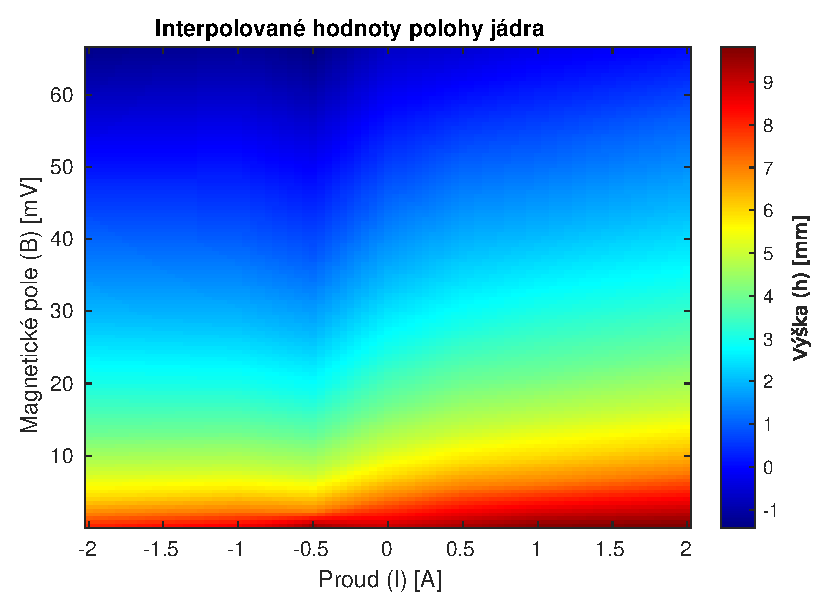
\includegraphics[width=0.9\textwidth]{kapitola6/Figures/hall_on_core_map.eps}
	\caption{Funkce využitá pro určení polohy jádra prvního prototypu}
	\label{fig::hall_oncore_map}
\end{figure}

Ačkoliv tento způsob umístění a řízení polohy jádra voicecoilu fungoval,
jeho největší nevýhodou bylo obtížnější integrace Hallovy sondy do jádra a
také by do útrob jádra musely vést 3 vodiče navíc,
což by ztěžovalo výrobu a montáž.
Bylo tedy přistoupeno k alternativnímu umístění sondy.

\subsection{Měření indukce permanentního magnetu umístěného zvenku voicecoilu}
\label{section::hall_perm_magnet}


V druhém prototypu voicecoilu byl došlo k umístění permanentního neodymového magnetu na statickém magnetickém obvodu jádra.
Hallova sonda byla umístěna na nástavbě připěvněné na pohyblivém jádře.
Motivací k tomuto umístění je nezávislost magnetické indukce na proudu,
což umožňuje přímo měřit polohu jádra bez ohledu na proud procházející cívkou,
ovšem nevýhodou je potřeba přidání permanenetního magnetu.

\begin{figure}[htbp]
	\centering
	\includegraphics[width=0.35\textwidth]{kapitola6/Figures/voicecoil.png}
	\caption{Druhý prototyp voicecoilu. V \textbf{červeném} poli umístěn permanentní magnet,
		v \textbf{modrém} poli pod plastovým krytem umístěna Hallova sonda.}
	\label{fig::voice_coil_second_prototype}
\end{figure}

Pro implementaci do mikrokontroléru bylo změřeno výstupní napětí Hallovy sondy při různých polohách jádra.
Výsledky měření byly interpolovány a zdiskretizovány do převodní \textit{LUT} tabulky,
což je v tomto případě pole, respektive pole, viz \oref{fig::hall_perm_magnet}.
Tato předpočítaná \textit{LUT} tabulka byla nahrána do mikrokontroléru.
Konkrétní implementace ve firmwaru je vidět v \nameref{section::position_regulator}.

\begin{figure}[htbp]
	\centering
	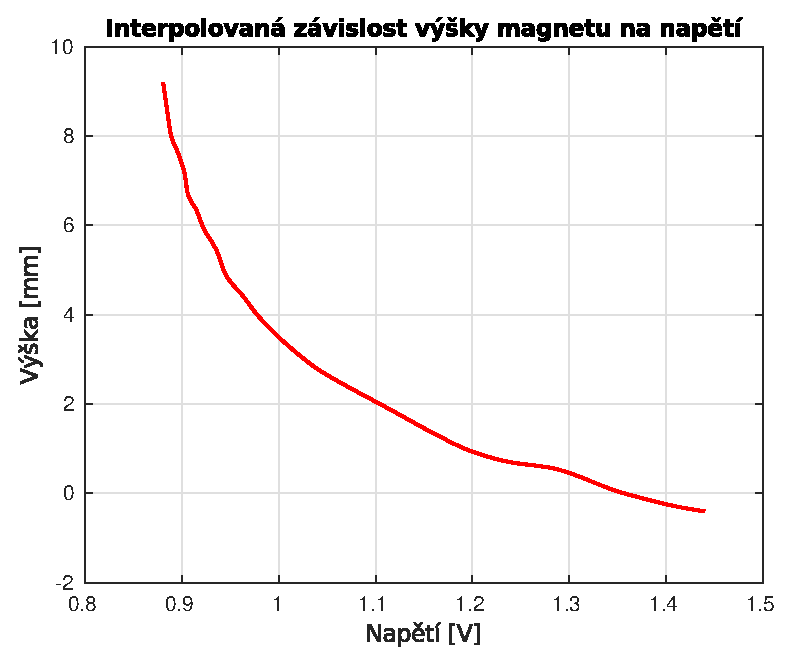
\includegraphics[width=0.9\textwidth]{kapitola6/Figures/hall_perm_magnet2.eps}
	\caption{Funkce využitá pro určení polohy jádra druhého prototypu}
	\label{fig::hall_perm_magnet}
\end{figure}


\subsection{Přesun součástek}

Omtimální nastavení frekvence a amplitudy kmitů, případně fázového posunu mezi jednotlivými voicecoily,
je závislé na velikosti a hmotnosti součástek, které mají být přesouvány.
V ideálním případě by mělo být nastavování těchto parametrů automatizováno,
například pomocí algoritmu, který by na základě snímání polohy součástek skrze kameru,
určil nastavení proudových zdrojů.
Hledání optimálního nastavení pro přesun součástek je však mimo rámec této práce.


\newpage
\chapter{Aplikace Staff 2.0}

Aplikace \textit{Staff 2.0} primárně slouží ke konfiguraci a řízení výstupních proudů zařízení \emph{MoSeZ}.
Kromě toho implementuje mechanismy pro detekci a správu připojených zařízení prostřednictvím sériové komunikace.
Aktivně monitoruje příchozí zprávy, na jejichž základě rozpoznává přítomnost a aktivitu jednotlivých jednotek.

Vývoj aplikace vycházel z první verze \textit{Staff}, která byla vytvořena pro prototyp zařízení \emph{MoSeZ}.
Pro tvorbu obou verzí aplikací bylo použito vývojové prostředí \textit{Matlab App Designer}.


\section{Obsluha aplikace}


Po spuštění počítače je nejprve nutné zvolit ve výběrovém seznamu (\textit{droplistu}) správný komunikační port,
který odpovídá připojenému převodníku \textit{USB-CAN} nebo \textit{USB-UART}.
Po výběru portu uživatel klikne na tlačítko \textit{Connect}, čímž aplikace zahájí sledování zpráv na sériovém rozhraní.
Zprávy mohou být přenášeny přímo přes \textit{CAN} nebo se může jednat o výpis zpráv z \textit{CAN} na \textit{UART}.

Aplikace na základě příchozích zpráv automaticky rozpozná připojená zařízení a pro každé z nich vytvoří odpovídající ovládací prvky v uživatelském rozhraní.
Pro každý zdroj může uživatel konfigurovat parametry jako výstupní proud, typ výstupu (\textit{DC/AC}), frekvenci, fázi, offset, a další.

Zapnutí a vypnutí konkrétního zdroje se provádí kliknutím na jeho \textit{ID label} v grafickém rozhraní.
V případě, že některé z připojených zařízení přestane pravidelně odesílat zprávy typu \textit{Heartbeat},
je po uplynutí definovaného časového limitu (aktuálně 15 sekund) automaticky označeno jako neaktivní a jeho ovládací prvky jsou z rozhraní odstraněny.

Tento mechanismus zajišťuje, že uživatelské rozhraní vždy odráží aktuální stav připojených zařízení,
a umožňuje dynamickou správu měnícího se počtu jednotek v síti bez nutnosti ručního zásahu.


\section{Detekce připojených zařízení}

Klíčovou roli v příjmu a zpracování dat ze sériové linky hraje funkce \texttt{serialRx}.
Tato metoda dekóduje přicházející zprávy a hledá identifikátory zařízení (\textit{ID label}), které slouží k automatické detekci připojených jednotek \emph{MoSeZ}.

\subsection{Formáty zpráv}

Pro účely detekce zařízení se využívají následující formáty zpráv:

\begin{table}[h!]
	\centering
	\caption{Přehled formátů zpráv použitých k detekci zařízení}
	\begin{tabular}{|l|l|l|}
		\hline
		\textbf{Typ zprávy} & \textbf{Formát}             & \textbf{Příklad}          \\ \hline
		Heartbeat           & \texttt{254HB<ID>}          & \texttt{254HB3}           \\ \hline
		Zpráva s ID         & \texttt{<ID>ID...}          & \texttt{3IDxx}            \\ \hline
		Teplotní zpráva     & \texttt{<ID>ID Temp: <v> C} & \texttt{3ID Temp: 27.5 C} \\ \hline
	\end{tabular}
	\label{tab:mosz_messages}
\end{table}

\begin{figure}[htbp]
	\centering
	\includegraphics[width=0.9\textwidth]{kapitola7/Figures/staff_connecting_sources.png}
	\caption{Ukázka přidávání zdrojů v aplikaci Staff 2.0 na základě činnosti na \textit{CAN} sběrnici}
	\label{fig:aplikace_staff_connecting}
\end{figure}

Po rozpoznání ID zařízení ve zprávě je volána funkce \texttt{handleDeviceMessage},
která aktualizuje vnitřní stav aplikace. Konkrétně aktualizuje pole \texttt{connected\_sources},
které udržuje informace o aktuálně připojených jednotkách.
Při detekci nového zařízení aplikace dynamicky vytvoří v uživatelském rozhraní odpovídající ovládací prvky pomocí funkce \texttt{addNewMosezRow}.,
například:

\begin{itemize}
	\item Přepínací tlačítko pro aktivaci/deaktivaci výstupu.
	\item Spinner pro nastavení proudu.
	\item Tlačítka pro volbu výstupu DC/AC.
	\item Volbu průběhu pro AC výstup.
	\item Spinnery pro parametry jako frekvence, offset, fáze a u obdélníku navíc střída a sklon hran.
\end{itemize}

\section{Zpracování neaktivity a odstranění zařízení}

Detekce neaktivních zařízení je zajištěna pomocí periodického časovače \texttt{updateTimer},
který spouští metodu \texttt{updateSourceRows}.
Ta kontroluje čas poslední zprávy ze zařízení a porovnává jej s prahovou hodnotou \texttt{inactivityThreshold} (aktuálně 15 sekund).
Pokud je zařízení neaktivní, volá se \texttt{deleteMoSeZRow}, čímž jsou jeho ovládací prvky odstraněny z GUI.

\begin{figure}[htbp]
	\centering
	\includegraphics[width=0.9\textwidth]{kapitola7/Figures/staff_sources_timeout.png}
	\caption{Ukázka odstranění neaktivních zařízení v aplikaci Staff 2.0}
	\label{fig:aplikace_staff_disconnecting}
\end{figure}

Dále funkce \texttt{compactGridLayout} a \texttt{sortSourceRows} dynamicky upravují rozložení GUI při změně počtu zařízení.
Výšku jednotlivých řádků upravuje \texttt{updateGridRowHeights},
čímž je zajištěno správné zobrazení ovládacích prvků i při velkém počtu připojených jednotek.

\section{Možnosti rozšíření}

Aplikace by rovněž mohla zobrazovat historická data (např.  proudové a teplotní křivky) nebo graficky zvýrazňovat stav zařízení.
Vylepšené hlášení chyb a systém notifikací by dále zlepšily použitelnost.
Pokud by bylo potřeba provozovat aplikaci i na počítačích bez \textit{Matlabu},
bylo by vhodné opustit \textit{Matlab App Designer} a přejít na alternativní platformu,
jako například jako například \textit{Python} s knihovnami \textit{PyQt} nebo \textit{Tkinter} pro desktopové \textit{GUI},
nebo \textit{C\#} s frameworky \textit{.NET MAUI} či \textit{WPF} pro multiplatformní desktopové aplikace.


\chapter{Závěr}

Tato diplomová práce se zaměřila na návrh, vývoj a testování rozšířené verze modulární platformy \emph{MoSeZ} určené pro řízení elektromagnetických aktuátorů.
Byly navrženy nové hardwarové moduly jednokanálového proudového zdroje s cílem zvýšit výkon, spolehlivost a flexibilitu systému.
Zvláštní důraz byl kladen na konstrukci výstupních proudových obvodů, implementaci bezpečnostních funkcí,
podporu střídavých proudů prostřednictvím \textit{DDS} a rozšíření možností řízení pomocí \textit{PID} regulace.

Platforma \textit{MoSeZ} nadále zachovává svou modulárnost -- jednotlivé jednokanálové moduly lze propojit pomocí sběrnice \textit{CAN} tak,
že se z pohledu uživatele chovají jako vícekanálový proudový zdroj.
Tato vlastnost umožňuje snadnou integraci platformy do větších řídicích systémů.

Těchto vlastností bylo využito při aplikaci ve vibračním podavači firmy \emph{DESSEQ},
kde čtyři moduly \emph{MoSeZ} řízené přes převodník \textit{USB-CAN} napájejí čtyři \textit{voicecoily}.
Pro zajištění bezpečného pohybu jádra bylo implementováno měření polohy pomocí Hallova senzoru,
které umožňuje přímo řídit polohu jádra a tím zabraňuje nárazu jádra do mechanických dorazů.

Dále byla vyvinuta nová desktopová aplikace \textit{Staff 2.0}, 
která poskytuje přehledné grafické rozhraní pro konfiguraci proudových výstupů, 
a ladění systému v reálném čase.
Aplikace automaticky detekuje zařízení dostupná na sběrnici podle jejich identifikátorů
a podporuje komunikaci přes převodníky \textit{USB-UART} i \textit{USB-CAN}.

Funkčnost navrženého systému byla ověřena sérií měření zaměřených na výstupní proudy, harmonické zkreslení, účinnost a přesnost regulace.
Výsledky potvrdily, že zařízení splňuje požadavky na přesné řízení proudových výstupů pro elektromagnetické aktuátory.

Do budoucna lze zvážit implementaci pokročilejších regulačních algoritmů
či návrh nové generace \textit{DPS} optimalizované s ohledem na elektromagnetickou kompatibilitu a platné \textit{EMC} normy.

%https://www.overleaf.com/learn/latex/Biblatex_bibliography_styles
\renewcommand\bibname{Seznam použité literatury}
\printbibliography
\addcontentsline{toc}{chapter}{Seznam použité literatury}
    
%Umisť na novou stránku
\clearpage
% Změna stylu "číslování" stránek
\pagenumbering{Alph}
% Přidání odkazu do obsahu
\addcontentsline{toc}{chapter}{Přílohy}

\section*{Příloha A}

\begin{figure}[H]
	\centering
	\includegraphics[width=\linewidth,page=1]{prilohy/prilohaA/schema.pdf}
	\caption{Schéma zdroje MoSeZ Rev. B}
	\label{priloha:schema_root}
\end{figure}


\begin{figure}[H]
	\centering
	\includegraphics[width=\linewidth,page=2]{prilohy/prilohaA/schema.pdf}
	\caption{Schéma části \emph{Input} zdroje MoSeZ Rev. B}
	\label{priloha:schema_Input}
\end{figure}
\begin{figure}[H]
	\centering
	\includegraphics[width=\linewidth,page=3]{prilohy/prilohaA/schema.pdf}
	\caption{Schéma části \emph{LMA38010} zdroje MoSeZ Rev. B}
	\label{priloha:schema_LMA38010}
\end{figure}
\begin{figure}[H]
	\centering
	\includegraphics[width=\linewidth,page=4]{prilohy/prilohaA/schema.pdf}
	\caption{Schéma části \emph{LM78M33} zdroje MoSeZ Rev. B}
	\label{priloha:schema_LM78M33}
\end{figure}
\begin{figure}[H]
	\centering
	\includegraphics[width=\linewidth,page=5]{prilohy/prilohaA/schema.pdf}
	\caption{Schéma části \emph{ATSAME51J18} zdroje MoSeZ Rev. B}
	\label{priloha:schema_MCU}
\end{figure}
\begin{figure}[H]
	\centering
	\includegraphics[width=\linewidth,page=6]{prilohy/prilohaA/schema.pdf}
	\caption{Schéma části \emph{Current Output} zdroje MoSeZ Rev. B}
	\label{priloha:schema_CurrentOutput}
\end{figure}
\begin{figure}[H]
	\centering
	\includegraphics[width=\linewidth,page=7]{prilohy/prilohaA/schema.pdf}
	\caption{Schéma části \emph{Can Bus Driver} zdroje MoSeZ Rev. B}
	\label{priloha:schema_CanBusDriver}
\end{figure}
\begin{figure}[H]
	\centering
	\includegraphics[width=\linewidth,page=8]{prilohy/prilohaA/schema.pdf}
	\caption{Schéma části \emph{Interface} zdroje MoSeZ Rev. B}
	\label{priloha:schema_Interface}
\end{figure}

\begin{figure}[H]
	\centering
	\includegraphics[width=\linewidth,page=8]{prilohy/prilohaA/pcb_back.jpg}
	\caption{Zadní část DPS MoSeZ Rev. B}
	\label{priloha:pcb_back}
\end{figure}

\FloatBarrier % Vložit za definici sekce

\section*{Příloha B}
\label{prilohaB}

\begin{figure}[H]
	\centering
	\includegraphics[width=\linewidth]{prilohy/prilohaB/boxes_back.pdf}
	\caption{Zadní část krabiček pro MoSeZ Rev. B}
	\label{priloha:boxes_back}
\end{figure}

\begin{figure}[H]
	\centering
	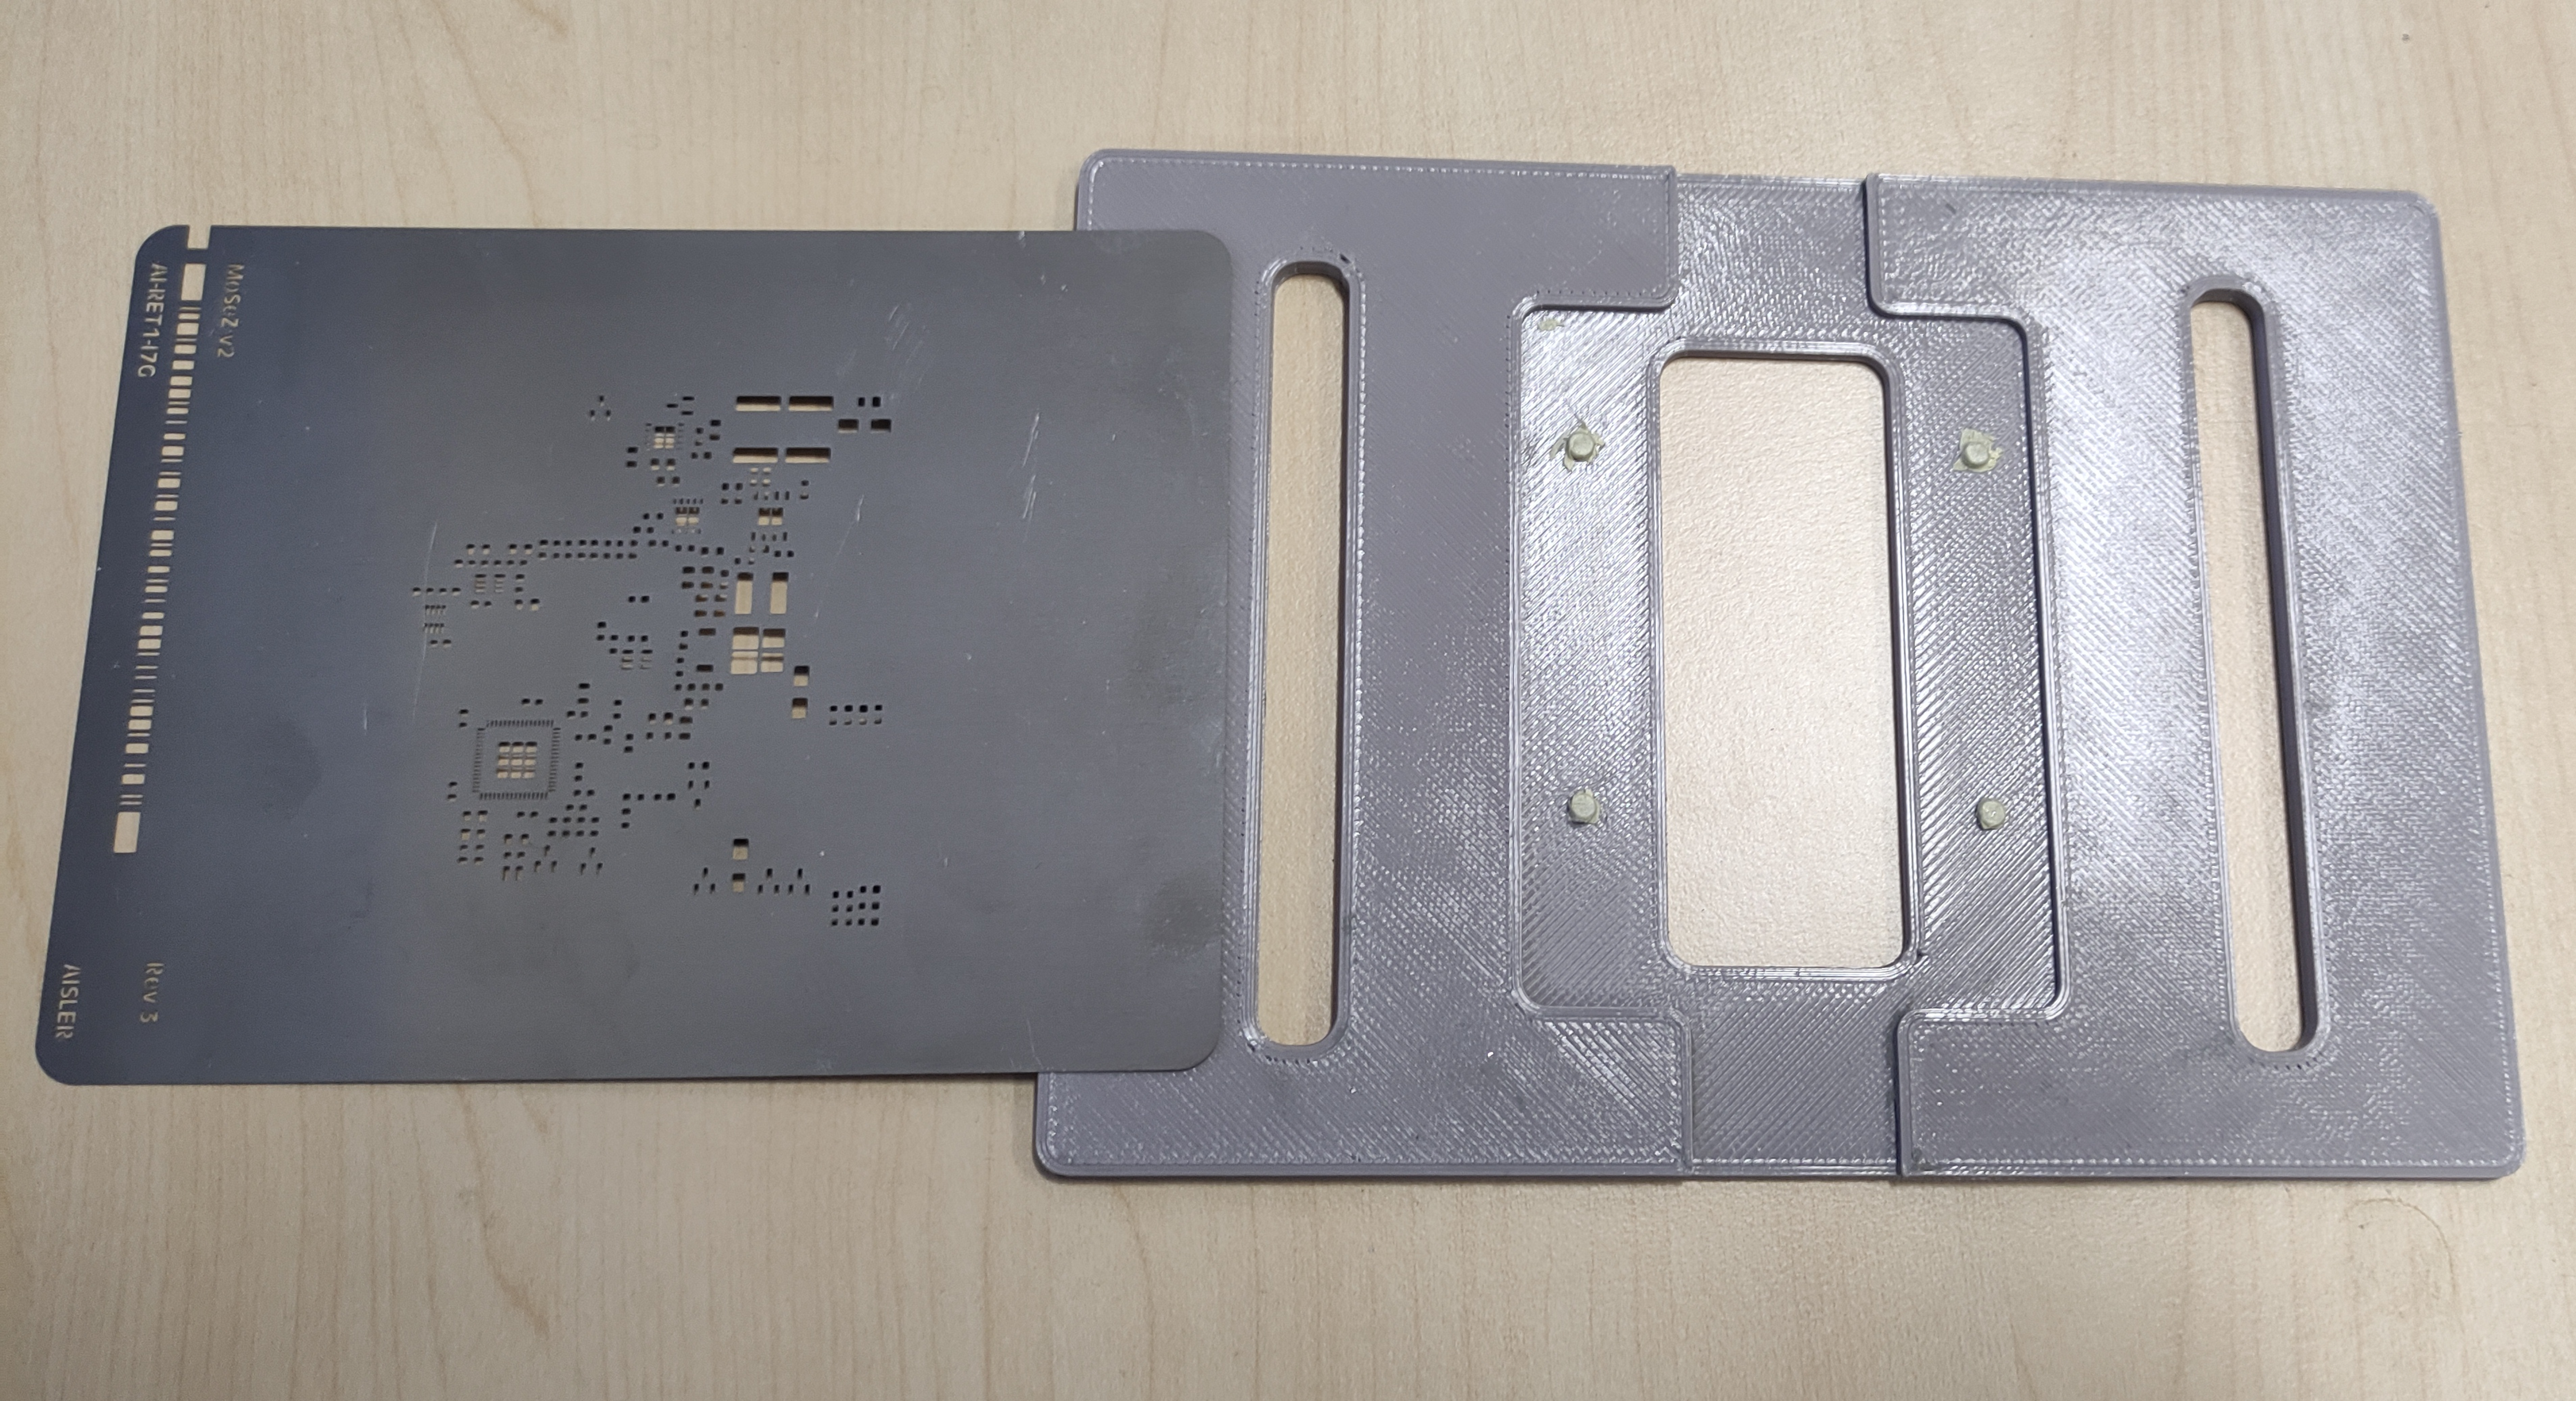
\includegraphics[width=\linewidth]{prilohy/prilohaB/paste_front.pdf}
	\caption{Držák DPS pro aplikaci pájecí pasty na přední stranu DPS}
	\label{priloha:dps_holder_paste}
\end{figure}

\FloatBarrier % Vložit za definici sekce

\section*{Příloha C}

\begin{figure}[H]
	\centering
	\includegraphics[width=\linewidth,page=1]{prilohy/prilohaC/emc_mozes.pdf}  % Replace 10 with last page number
	\caption{Vyzařování rušení na kmitočtech 30 – 1000 MHz desky MoSeZ Rev. B ve standby režimu}
	\label{priloha:mereni_emc_standby}
\end{figure}


\begin{figure}[H]
	\centering
	\includegraphics[width=\linewidth,page=7]{prilohy/prilohaC/emc_mozes.pdf}
	\caption{Vyzařování rušení na kmitočtech 30 – 1000 MHz desky MoSeZ Rev. B se zapnutým výstupem
	a připojeným vstupními a výstupními filtry}
	\label{priloha:mereni_emc_on}
\end{figure}


% Příloha přes celou stranu (pokud má PDF více stran, můžete je zde vyjmenovat pomocí pages={1,2,3} )
%\includepdf[pages={1}]{prilohy/PRILOHA.pdf}



\end{document}

